\documentclass[spanish,a4paper,11pt,oneside]{extreport}
% \documentclass[12pt,a4paper,oneside]{report}

% Fonts
% For use with XeLaTeX
\usepackage{amsmath}
\usepackage{fontspec}
\setmainfont[%
  Path              = ./fonts/ArgentumSans/,%
  Extension         = .ttf,
  UprightFont       = *-Light,
  BoldFont          = *-SemiBold, % ULL bold font
  ItalicFont        = *-LightItalic,
  BoldItalicFont    = *-SemiBoldItalic, % Linux Libertine O Regular Semibold Italic
  Scale             = 0.95%
]%
{hinted-ArgentumSans}

\usepackage[spanish,es-tabla]{babel} % Para español
\usepackage{csquotes} % Para mejorar el formato de las citas 
% \usepackage[backend=biber,style=ieee,sorting=none]{biblatex} % Activa IEEE

% \usepackage[utf8]{inputenc}
% Only with pdflatex

%\usepackage{alltt}

%\usepackage[ruled,vlined,commentsnumbered,linesnumbered,inoutnumbered,titlenotnumbered,noend]{algorithm2e}
%\SetKwRepeat{Do}{do}{while}
%
\usepackage{afterpage}
\usepackage{multirow}
\usepackage{array} 
%\usepackage{amsfonts}
\usepackage{amsmath}
%\usepackage{bigstrut}
%\usepackage{booktabs}
%\usepackage{caption}
%\usepackage{chngpage}
\usepackage{float}
\usepackage{enumitem,lipsum}
%\usepackage{graphicx}
%\usepackage{lscape}
%\usepackage{microtype}
%\usepackage{natbib}
\usepackage{pdflscape}
%\usepackage{rotating}
\usepackage{subcaption}
% \usepackage{subfigure}
%\usepackage{ctable}
\usepackage{hyperref}
%\usepackage{enumerate}
%\usepackage{gensymb}
\usepackage{eurosym}
\usepackage[scaled]{inconsolata} % fuente tipo consola
\usepackage{multicol}
\usepackage{listings}
\usepackage{xcolor}
\usepackage{longtable} % Para tablas que se dividen en múltiples páginas
\setlist[itemize]{itemsep=0pt,parsep=0pt}
\usepackage[hypcap=false]{caption}
\usepackage{tcolorbox}

\synctex=1

\setcounter{tocdepth}{3}
\setcounter{secnumdepth}{3}

%
%\usepackage{lineno}
%%\\linenumbers
%\setlength\linenumbersep{5pt}
%\renewcommand\linenumberfont{\normalfont\tiny\sffamily\color{gray}}

\usepackage[top=2.5cm, bottom=2.5cm, left=2.5cm, right=2.5cm]{geometry}

\newenvironment{sourcecode}
{\begin{list}{}{\setlength{\leftmargin}{1em}}\item\scriptsize\bfseries}
{\end{list}}

\newenvironment{littlesourcecode}
{\begin{list}{}{\setlength{\leftmargin}{1em}}\item\tiny\bfseries}
{\end{list}} 


\newenvironment{summary}
{\par\noindent\begin{center}\textbf{Abstract}\end{center}\begin{itshape}\par\noindent}
{\end{itshape}}

\newenvironment{keywords}
{\begin{list}{}{\setlength{\leftmargin}{1em}}\item[\hskip\labelsep \bfseries Keywords:]}
{\end{list}}

\newenvironment{palabrasClave}
{\begin{list}{}{\setlength{\leftmargin}{1em}}\item[\hskip\labelsep \bfseries Palabras clave:]}
{\end{list}}

\usepackage{xcolor}
\usepackage{listings}
\renewcommand{\lstlistingname}{Listado}
\lstloadlanguages{Python}
\lstset{
  language=Python,                      % Python language
  basicstyle=\small\ttfamily,           % Listados en small y monoespaciado
  keywordstyle=\color{blue},            % Palabras clave en azul
  identifierstyle=\color{black},        % Identificadores en negro
  commentstyle=\color{green!50!black},  % Comentarios en verde oscuro
  stringstyle=\color{red},              % Cadenas en rojo
  showstringspaces=false,
  frame=tb,
  captionpos=b,
  belowcaptionskip=12pt,
  stepnumber=1,                         % Opciones de líneas y etiquetas
  numbers=left, 
  numberstyle=\scriptsize,
  numbersep=5pt,
  tabsize=4                             % Tamaño de tabulación
}

\colorlet{punct}{red!60!black}
\definecolor{background}{HTML}{EEEEEE}
\definecolor{delim}{RGB}{20,105,176}
\colorlet{numb}{magenta!60!black}

\lstdefinelanguage{json}{
    basicstyle=\normalfont\ttfamily,
    numbers=left,
    numberstyle=\scriptsize,
    stepnumber=1,
    numbersep=8pt,
    showstringspaces=false,
    breaklines=true,
    frame=lines,
    backgroundcolor=\color{background},
    literate=
     *{0}{{{\color{numb}0}}}{1}
      {1}{{{\color{numb}1}}}{1}
      {2}{{{\color{numb}2}}}{1}
      {3}{{{\color{numb}3}}}{1}
      {4}{{{\color{numb}4}}}{1}
      {5}{{{\color{numb}5}}}{1}
      {6}{{{\color{numb}6}}}{1}
      {7}{{{\color{numb}7}}}{1}
      {8}{{{\color{numb}8}}}{1}
      {9}{{{\color{numb}9}}}{1}
      {:}{{{\color{punct}{:}}}}{1}
      {,}{{{\color{punct}{,}}}}{1}
      {\{}{{{\color{delim}{\{}}}}{1}
      {\}}{{{\color{delim}{\}}}}}{1}
      {[}{{{\color{delim}{[}}}}{1}
      {]}{{{\color{delim}{]}}}}{1},
}

% Define RouterOS language for listings
% Define colors for RouterOS syntax highlighting (similar to YAML style)
\definecolor{roscommand}{RGB}{0,0,255}      % Blue for commands (like yamlkey)
\definecolor{rosvalue}{RGB}{0,128,0}        % Green for values
\definecolor{roscomment}{RGB}{128,128,128}  % Gray for comments
\definecolor{rosstring}{RGB}{255,0,0}       % Red for strings
\definecolor{rospath}{RGB}{128,0,128}       % Purple for paths like /system, /interface

% Define RouterOS language for listings with YAML-style formatting
\lstdefinelanguage{RouterOS}{
    keywords={interface, bridge, add, name, port, address, identity, set, enable, vlan, ethernet, find, ospf, instance, redistribute-connected, as-type-1, numbers, network, area, backbone, true, false, yes, no},
    keywordstyle=\color{roscommand}\bfseries,
    sensitive=true,
    comment=[l]{\#},
    morecomment=[s]{/*}{*/},
    commentstyle=\color{roscomment}\ttfamily,
    stringstyle=\color{rosstring}\ttfamily,
    moredelim=[s][\color{rosstring}]{"}{"},
    moredelim=[s][\color{rosstring}]{'}{'},
    morestring=[b]",
    morestring=[b]',
    % Highlight RouterOS paths
    moredelim=[s][\color{rospath}\bfseries]{/}{\ },
    basicstyle=\ttfamily\small,
    showstringspaces=false,
    showspaces=false,
    showtabs=false,
    frame=single,
    frameround=tttt,
    rulecolor=\color{black},
    backgroundcolor=\color{gray!10},
    breaklines=true,
    breakatwhitespace=true,
    tabsize=2,
    numbers=left,
    numberstyle=\tiny\color{gray},
    stepnumber=1,
    numbersep=5pt,
    columns=fullflexible,
    keepspaces=true,
    alsoletter={=/},
}

% Set default style for RouterOS listings
\lstset{
  language=RouterOS,
}

% Define YAML language for listings
% Define colors for YAML syntax highlighting
\definecolor{yamlkey}{RGB}{0,0,255}
\definecolor{yamlvalue}{RGB}{0,128,0}
\definecolor{yamlcomment}{RGB}{128,128,128}
\definecolor{yamlstring}{RGB}{255,0,0}

% Define YAML language for listings
\lstdefinelanguage{yaml}{
  keywords={true,false,null,yes,no},
  keywordstyle=\color{yamlkey}\bfseries,
  basicstyle=\ttfamily\small,
  sensitive=true,
  comment=[l]{\#},
  commentstyle=\color{yamlcomment}\ttfamily,
  stringstyle=\color{yamlstring}\ttfamily,
  moredelim=[s][\color{yamlstring}]{"}{"},
  moredelim=[s][\color{yamlstring}]{'}{'},
  morestring=[b]",
  morestring=[b]',
  showstringspaces=false,
  showspaces=false,
  showtabs=false,
  frame=single,
  frameround=tttt,
  rulecolor=\color{black},
  backgroundcolor=\color{gray!10},
  breaklines=true,
  breakatwhitespace=true,
  tabsize=2,
  numbers=left,
  numberstyle=\tiny\color{gray},
  stepnumber=1,
  numbersep=5pt,
}

% Set default style for YAML listings
\lstset{
  language=yaml
}

% Cisco IOS language for listings
% Define colors for Cisco IOS syntax highlighting (similar to YAML style)
\definecolor{ciscocommand}{RGB}{0,0,255}      % Blue for commands
\definecolor{ciscovalue}{RGB}{0,128,0}        % Green for values/parameters
\definecolor{ciscocomment}{RGB}{128,128,128}  % Gray for comments
\definecolor{ciscostring}{RGB}{255,0,0}       % Red for strings
\definecolor{ciscomode}{RGB}{128,0,128}       % Purple for configuration modes
\definecolor{ciscokeyword}{RGB}{0,64,128}     % Dark blue for keywords

% Define Cisco IOS language for listings
% Define colors for Cisco IOS syntax highlighting
\definecolor{ciscoblue}{RGB}{0,102,204}
\definecolor{ciscogreen}{RGB}{0,128,0}
\definecolor{ciscored}{RGB}{204,0,0}
\definecolor{ciscoorange}{RGB}{255,102,0}
\definecolor{ciscogray}{RGB}{128,128,128}

% Define the Cisco IOS language
\lstdefinelanguage{CiscoIOS}{
  % Keywords - Configuration commands
  morekeywords=[1]{
    interface, router, ip, access-list, line, enable, configure, terminal,
    hostname, banner, service, no, shutdown, exit, end, write, copy,
    running-config, startup-config, show, debug, clear, reload, boot,
    version, username, password, secret, clock, logging, snmp-server,
    ntp, spanning-tree, vlan, switchport, trunk, access, voice,
    crypto, isakmp, ipsec, transform-set, map, policy, key, string,
    peer, address, group, lifetime, authentication, encryption,
    negotiation, proposal, security, association, tunnel, mode,
    transport, esp, ah, md5, sha, des, 3des, aes
  },
  % Keywords - Interface types and protocols
  morekeywords=[2]{
    FastEthernet, GigabitEthernet, TenGigabitEthernet, Serial, Loopback,
    Tunnel, Vlan, Port-channel, Dialer, ATM, Frame-Relay, Ethernet,
    ospf, eigrp, rip, bgp, isis, static, connected, summary,
    redistribute, network, area, process-id, autonomous-system,
    neighbor, route-map, prefix-list, community-list, as-path,
    tcp, udp, icmp, http, https, ssh, telnet, ftp, tftp, smtp,
    dns, dhcp, nat, pat, vpn, gre, l2tp, pptp
  },
  % Keywords - Show commands and status
  morekeywords=[3]{
    running, startup, flash, version, interfaces, protocols,
    route, arp, mac, address-table, vlan, spanning-tree,
    access-lists, crypto, sessions, users, processes, memory,
    cpu, utilization, inventory, license, tech-support,
    brief, detail, summary
  },
  % Keywords - Common parameters and values  
  morekeywords=[4]{
    permit, deny, any, host, eq, gt, lt, neq, range, log,
    established, fragments, precedence, tos, dscp, cos,
    full-duplex, half-duplex, auto, speed, duplex, mtu,
    encapsulation, dot1q, isl, native, allowed, pruning,
    rapid-pvst, pvst, mstp, rstp, stp, portfast, bpduguard,
    root, priority, cost, hello-time, forward-delay, max-age
  },
  % Comments
  morecomment=[l]{!},
  morecomment=[s]{/*}{*/},
  % Strings
  morestring=[b]",
  morestring=[b]',
  % Additional settings
  sensitive=false,
  breaklines=true,
  breakatwhitespace=true,
  showstringspaces=false,
  numbers=left,
  numberstyle=\tiny\color{ciscogray},
  stepnumber=1,
  tabsize=2,
  % Styling
  keywordstyle=[1]\color{ciscoblue}\bfseries,     % Main commands - blue bold
  keywordstyle=[2]\color{ciscogreen}\bfseries,    % Interfaces/protocols - green bold  
  keywordstyle=[3]\color{ciscoorange},            % Show commands - orange
  keywordstyle=[4]\color{ciscored},               % Parameters - red
  commentstyle=\color{ciscogray}\itshape,         % Comments - gray italic
  stringstyle=\color{ciscored},                   % Strings - red
  backgroundcolor=\color{gray!10},        % Light gray background
  frame=single,
  frameround=tttt,
  rulecolor=\color{ciscogray}
}

% Define a custom style for Cisco IOS
\lstdefinestyle{CiscoIOSStyle}{
  language=CiscoIOS,
  basicstyle=\ttfamily\footnotesize,
  keywordstyle=[1]\color{ciscoblue}\bfseries,
  keywordstyle=[2]\color{ciscogreen}\bfseries,
  keywordstyle=[3]\color{ciscoorange},
  keywordstyle=[4]\color{ciscored},
  commentstyle=\color{ciscogray}\itshape,
  stringstyle=\color{ciscored},
  backgroundcolor=\color{gray!10},
  frame=single,
  frameround=tttt,
  rulecolor=\color{ciscogray},
  numbers=left,
  numberstyle=\tiny\color{ciscogray},
  breaklines=true,
  breakatwhitespace=true,
  showstringspaces=false,
  tabsize=2,
  captionpos=b
}

% Define Docker language for listings
\lstdefinelanguage{Dockerfile}{
  keywords={
    FROM,
    MAINTAINER,
    RUN,
    CMD,
    LABEL,
    EXPOSE,
    ENV,
    ADD,
    COPY,
    VOLUME,
    USER,
    WORKDIR,
    ARG,
    ONBUILD,
    STOPSIGNAL,
    HEALTHCHECK,
    SHELL
  },
  morecomment=[l]{\#},
  string=[s]{"}{"},
  string=[s]{'}{'},
  sensitive=true,
  keepspaces=false, % To prevent issues with indents in instructions
  commentstyle=\color{gray}\ttfamily,
  keywordstyle=\color{blue}\bfseries,
  stringstyle=\color{orange}\ttfamily,
  identifierstyle=\color{black}\ttfamily,
}

% Espaciado entre parrafo y lineas.
% Modificar mas abajo, antes del resumen
%\setlength{\parindent}{4em}
%\setlength{\parskip}{10pt}
\renewcommand{\baselinestretch}{1.1}

% Espaciado entre numero de titulo y titulo
\makeatletter
\newcommand\mylistoffigures{%
  \if@twocolumn
    \@restonecoltrue\onecolumn
  \else
    \@restonecolfalse
  \fi
  \chapter*{\listfigurename
    \@mkboth{\MakeUppercase\listfigurename}%
        {\MakeUppercase\listfigurename}}%
  \begingroup
    \let\oldnumberline\numberline
    \renewcommand{\numberline}[1]{##1.\hspace{0.5em}}%
    \@starttoc{lof}%
  \endgroup
  \if@restonecol\twocolumn\fi
}
\newcommand\mylistoftables{%
  \if@twocolumn
    \@restonecoltrue\onecolumn
  \else
    \@restonecolfalse
  \fi
  \chapter*{\listtablename
    \@mkboth{\MakeUppercase\listtablename}%
        {\MakeUppercase\listtablename}}%
  \begingroup
    \let\oldnumberline\numberline
    \renewcommand{\numberline}[1]{##1.\hspace{0.5em}}%
    \@starttoc{lot}%
  \endgroup
  \if@restonecol\twocolumn\fi
}
\makeatother


\begin{document}

\renewcommand\listtablename{Índice de Tablas}
\renewcommand\listfigurename{Índice de Figuras}

%%%%%%%%%%%%%%%%%%%%%%%%%%%%%%%%%%%%%%%%%%%%%%%%%%%%%%%%%%%%%%%%%%%%%%%%%%%%%%%
% First Page
%%%%%%%%%%%%%%%%%%%%%%%%%%%%%%%%%%%%%%%%%%%%%%%%%%%%%%%%%%%%%%%%%%%%%%%%%%%%%%%
\pagestyle{empty}
\thispagestyle{empty}


\newcommand{\HRule}{\rule{\linewidth}{1mm}}
\setlength{\parindent}{0mm}
\setlength{\parskip}{0mm}

\vspace*{\stretch{0.5}}

\begin{center}
	
\includegraphics[scale=0.8]{images/escuela-ingenieria-tecnologia-original}\\[10mm]
	{\Huge\bf  Trabajo de Fin de Grado}
\end{center}

\HRule
\begin{center}
	{\Huge Diseño de infraestructura de red para una empresa multisede} \\[3.5mm]
	{\Large \textit{Design of network infrastructure for a multi-site company}} \\[5mm]
	{\Large Cheuk Kelly Ng Pante} \\[5mm]


\end{center}
\HRule
\vspace*{\stretch{2}}
\begin{center}
	\Large La Laguna, \today
\end{center}

\setlength{\parindent}{5mm}

%%%%%%%%%%%%%%%%%%%%%%%%%%%%%%%%%%%%%%%%%%%%%%%%%%%%%%%%%%
% Signature page (add the official stamp)
%%%%%%%%%%%%%%%%%%%%%%%%%%%%%%%%%%%%%%%%%%%%%%%%%%%%%%%%%%

%%%%%%%%%%%%%%%%%%%%%%%%%%%%%%%%%%%%%%%%%%%%%%%%%%%%%%%%%%
\newpage
\thispagestyle{empty}
\vspace*{\fill}
\begin{center}
  % Página intencionadamente en blanco
\end{center}
\vspace*{\fill}
\newpage
%%%%%%%%%%%%%%%%%%%%%%%%%%%%%%%%%%%%%%%%%%%%%%%%%%%%%%%%%%

\newpage
\thispagestyle{empty}

D. {\bf Jonás Philipp Lüke}, profesor contratado Doctor de Universidad adscrito al Departamento de Ingeniería Industrial de la Universidad de La Laguna, como tutor.

\bigskip
\bigskip
{\bf C E R T I F I C A}

\bigskip
\bigskip

Que la presente memoria titulada:

\bigskip
''{\it Diseño de infraestructura de red para una empresa multisede}''

\bigskip
\bigskip
\bigskip

\noindent ha sido realizada bajo su dirección por D. {\bf Cheuk Kelly Ng Pante}.

\bigskip
\bigskip

Y para que así conste, en cumplimiento de la legislación vigente y a los efectos
oportunos firman la presente en La Laguna a \today

%%%%%%%%%%%%%%%%%%%%%%%%%%%%%%%%%%%%%%%%%%%%%%%%%%%%%%%%%%

%%%%%%%%%%%%%%%%%%%%%%%%%%%%%%%%%%%%%%%%%%%%%%%%%%%%%%%%%%
\newpage
\thispagestyle{empty}
\vspace*{\fill}
\begin{center}
  % Página intencionadamente en blanco
\end{center}
\vspace*{\fill}
\newpage
%%%%%%%%%%%%%%%%%%%%%%%%%%%%%%%%%%%%%%%%%%%%%%%%%%%%%%%%%%


\newpage
\thispagestyle{empty}

{ \flushright

	\begin{LARGE}
		\textbf{Agradecimientos}
	\end{LARGE}

	\hspace{3mm}

	En primer lugar, quiero agradecer profundamente a mi tutor Jonás Philipp Lüke, por aceptar la
	realización de este proyecto y por su apoyo constante durante todo el proceso. Su orientación,
	conocimientos y experiencia han sido fundamentales para el desarrollo de este trabajo.

	\vspace{0.5cm}
	También quiero agradecer a todas las amistades que he ido haciendo a lo largo de mi carrera, que me han
	brindado su apoyo y amistad. Su compañía y apoyo han sido una fuente de inspiración y motivación constante.

	\vspace{0.5cm}
	Por último, quiero agradecer a mi familia, que siempre ha estado ahí para mí, brindándome su amor
	y apoyo incondicional. Su confianza en mí y su aliento constante me han dado la fuerza necesaria para
	completar este proyecto y alcanzar mis metas académicas.
}
%%%%%%%%%%%%%%%%%%%%%%%%%%%%%%%%%%%%%%%%%%%%%%%%%%%%%%%%

%%%%%%%%%%%%%%%%%%%%%%%%%%%%%%%%%%%%%%%%%%%%%%%%%%%%%%%%%%
\newpage
\thispagestyle{empty}
\vspace*{\fill}
\begin{center}
  % Página intencionadamente en blanco
\end{center}
\vspace*{\fill}
\newpage
%%%%%%%%%%%%%%%%%%%%%%%%%%%%%%%%%%%%%%%%%%%%%%%%%%%%%%%%%%


\newpage
\thispagestyle{empty}

\bigskip
\begin{center}
  \begin{LARGE}
    \textbf{Licencia}
  \end{LARGE}
\end{center}

\bigskip
\bigskip
\bigskip
% * Si quiere permitir que se compartan las adaptaciones de tu obra mientras se comparta de la misma manera y quieres permitir usos comerciales de tu obra (licencia de Cultura Libre) indica:

\begin{center}
	
\includegraphics[scale=1.8]{images/by-sa_88x31}\\[5mm]
\end{center}

\begin{center}
	© Esta obra está bajo una licencia de Creative Commons \\
	Reconocimiento-CompartirIgual 4.0 Internacional.
\end{center}

%%%%%%%%%%%%%%%%%%%%%%%%%%%%%%%%%%%%%%%%%%%%%%%%%%%%%%%%

%%%%%%%%%%%%%%%%%%%%%%%%%%%%%%%%%%%%%%%%%%%%%%%%%%%%%%%%%%
\newpage
\thispagestyle{empty}
\vspace*{\fill}
\begin{center}
  % Página intencionadamente en blanco
\end{center}
\vspace*{\fill}
\newpage
%%%%%%%%%%%%%%%%%%%%%%%%%%%%%%%%%%%%%%%%%%%%%%%%%%%%%%%%%%

\newpage
\thispagestyle{empty}

% Resumen obligatorio

\begin{abstract}
{\em
Este proyecto presenta el diseño y simulación de una infraestructura red, orientada a la 
mejora de la conectividad y la gestión centralizada de una organización con varias sedes. Este estudio 
propone una arquitectura de red moderna, escalable y segura; diseñada conforme a las necesidades 
actuales de comunicación y gestión tecnológica en entornos distribuidos.

\vspace{0.5cm}
\noindent
Para ello, se han empleado herramientas de simulación para validar el funcionamiento del diseño, incluyendo
la implementación de protocolos de enrutamiento o servicios de red internos. El resultado ha sido
una solución escalable y adaptable, alineada con los requisitos técnicos y operativos de una red
corporativa moderna.
}

\begin{palabrasClave}
GNS3, Infraestructura, Interconexión, IPv6, Redes corporativas, SD-WAN, VPN, VoIP
\end{palabrasClave}

\end{abstract}
%%%%%%%%%%%%%%%%%%%%%%%%%%%%%%%%%%%%%%%%%%%%%%%%%%%%%%%%%

%%%%%%%%%%%%%%%%%%%%%%%%%%%%%%%%%%%%%%%%%%%%%%%%%%%%%%%%%

%%%%%%%%%%%%%%%%%%%%%%%%%%%%%%%%%%%%%%%%%%%%%%%%%%%%%%%%%%
\newpage
\thispagestyle{empty}
\vspace*{\fill}
\begin{center}
  % Página intencionadamente en blanco
\end{center}
\vspace*{\fill}
\newpage
%%%%%%%%%%%%%%%%%%%%%%%%%%%%%%%%%%%%%%%%%%%%%%%%%%%%%%%%%%

\newpage
\vspace*{200pt}
\thispagestyle{empty}

% Summary in english is compulsory

\begin{summary}
{\em
\noindent
This project presents the design and simulation of a network infrastructure, aimed at improving 
connectivity and centralised management of a multi-site organisation. This study proposes a modern, 
scalable and secure network architecture; designed according to the current needs 
of communication and technological management in distributed environments.

\vspace{0.5cm}
\noindent
Simulation tools have been used to validate the performance of the design, including the implementation
of routing protocols or internal network services. The result has been a scalable and adaptable 
solution, aligned with the technical and operational requirements of a modern corporate network.
}

\em
\begin {keywords}
GNS3, Infrastructure, Interconnection, IPv6, Corporate Networks, SD-WAN, VPN, VoIP
\end {keywords}

\end{summary}

%%%%%%%%%%%%%%%%%%%%%%%%%%%%%%%%%%%%%%%%%%%%%%%%%%%%%%%%%%
\newpage
\thispagestyle{empty}
\vspace*{\fill}
\begin{center}
  % Página intencionadamente en blanco
\end{center}
\vspace*{\fill}
\newpage
%%%%%%%%%%%%%%%%%%%%%%%%%%%%%%%%%%%%%%%%%%%%%%%%%%%%%%%%%%

%%%%%%%%%%%%%%%%%%%%%%%%%%%%%%%%%%%%%%%%%%%%%%%%%%%%%%%%%

%%%%%%%%%%%%%%%%%%%%%%%%%%%%%%%%%%%%%%%%%%%%%%%%%%%%%%%%%
\newpage{\pagestyle{empty}}
\thispagestyle{empty}
%%%%%%%%%%%%%%%%%%%%%%%%%%%%%%%%%%%%%%%%%%%%%%%%%%%%%%%%%
\pagestyle{myheadings} %my head defined by markboth or markright
% No funciona bien \markboth sin "twoside" en \documentclass, pero al
% ponerlo se dan un montón de errores de underfull \vbox, con lo que no se
% ha puesto.


%%Aqui debería poner el nombre del proyecto pero, como es muy grande no cabe y se ve feo en el PDF
\markboth{xxxxx}{}

%%%%%%%%%%%%%%%%%%%%%%%%%%%%%%%%%%%%%%%%%%%%%%%%%%%%%%%%%
%Numeracion en romanos
\renewcommand{\thepage}{\roman{page}}
\setcounter{page}{1}
\pagestyle{plain}

%%%%%%%%%%%%%%%%%%%%%%%%%%%%%%%%%%%%%%%%%%%%%%%%%%%%%%%%%

\tableofcontents

%%%%%%%%%%%%%%%%%%%%%%%%%%%%%%%%%%%%%%%%%%%%%%%%%%%%%%%%%
%%%%%%%%%%%%%%%%%%%%%%%%%%%%%%%%%%%%%%%%%%%%%%%%%%%%%%%%%%
\newpage
\thispagestyle{empty}
\vspace*{\fill}
\begin{center}
  % Página intencionadamente en blanco
\end{center}
\vspace*{\fill}
\newpage
%%%%%%%%%%%%%%%%%%%%%%%%%%%%%%%%%%%%%%%%%%%%%%%%%%%%%%%%%%

\newpage{\pagestyle{empty}}

\mylistoffigures
% \listoffigures

%%%%%%%%%%%%%%%%%%%%%%%%%%%%%%%%%%%%%%%%%%%%%%%%%%%%%%%%%
\newpage{\pagestyle{empty}}

\mylistoftables
% \listoftables

%%%%%%%%%%%%%%%%%%%%%%%%%%%%%%%%%%%%%%%%%%%%%%%%%%%%%%%%%%
\newpage
\thispagestyle{empty}
\vspace*{\fill}
\begin{center}
  % Página intencionadamente en blanco
\end{center}
\vspace*{\fill}
\newpage
%%%%%%%%%%%%%%%%%%%%%%%%%%%%%%%%%%%%%%%%%%%%%%%%%%%%%%%%%%

%%%%%%%%%%%%%%%%%%%%%%%%%%%%%%%%%%%%%%%%%%%%%%%%%%%%%%%%%%%%%%%%%%%%%%%%%%%%%%%
\newpage{\pagestyle{empty}}

%%%%%%%%%%%%%%%%%%%%%%%%%%%%%%%%%%%%%%%%%%%%%%%%%%%%%%%%%%%%%%%%%%%%%%%%%%%%%%%
\newpage
\thispagestyle{empty}

% Numeracion a partir del capitulo I
\renewcommand{\thepage}{\arabic{page}}
\setcounter{page}{1}
\pagestyle{plain}

\chapter{\LARGE Introducción}
\label{chapter:intro}

En la actualidad, la conectividad y la seguridad de las redes corporativas son pilares fundamentales para garantizar su correcto funcionamiento, es por ello, que la mayoría de las empresas están en un proceso de transformación digital. Por supuesto, aquellas organizaciones con varias sedes requieren de una infraestructura de red eficiente, robusta, escalable y que cuente con una comunicación segura entre ellas.

\vspace{0.5cm}
A medida que la tecnología sigue avanzando y los servicios en línea se vuelven parte esencial del día a día (como ocurre con la telefonía basada en IP, las plataformas en la nube o el acceso remoto a sistemas), se hace cada vez más necesario contar con redes que integren herramientas actuales, por lo que la elección de las tecnologías core adquieren un papel crucial. El objetivo es facilitar la interacción entre ubicaciones en diferentes áreas geográficas, lo cual permite que los datos se transmitan de manera eficiente entre redes y dispositivos. También es 
importante garantizar un tránsito de información ágil y confiable en toda la estructura de red.

\vspace{0.5cm}
La elección de la tecnología de interconexión adecuada depende de varios factores, como el tamaño de la red, el tipo de tráfico que se espera, la latencia o el ancho de banda requerido. Cada una de estas presenta sus propias ventajas y desventajas, y la selección de la más apropiada debe basarse en las necesidades específicas de la organización. Existen diversas tecnologías \cite{conexion_redes_extendidas}, como por ejemplo:
\begin{itemize}
  \item \textbf{ATM (Asynchronous Transfer Mode):} es la conjunción de las redes de conmutación de circuitos y de conmutación de paquetes, también conocida como ``cell relay''. Está basada principalmente en el concepto de conmutación de paquetes, pero con un tamaño fijo, y es capaz de prestar servicios que requieren una velocidad constante o prestaciones de la conmutación de circuitos, todo ello utilizando señalización por canal común.
  \item \textbf{Frame Relay:} es un protocolo WAN de alto rendimiento que funciona en las capas físicas y de enlace de datos del modelo de referencia OSI. Frame Relay reduce los costos de redes a través del uso de menos equipos, menos complejidad y una implementación más fácil. Proporciona un mayor ancho de banda, mejor fiabilidad y resistencia a fallas que las líneas privadas o arrendadas.
  \item \textbf{X.25:} es un estándar de protocolo de la Unión Internacional de Telecomunicaciones, Sector de Estandarización de Telecomunicaciones (ITU-T) para la comunicación WAN que define cómo los dispositivos de usuario y los dispositivos de red establecen y mantienen conexiones.
  \item \textbf{MPLS (Multiprotocol Label Switching):} es una técnica de alto rendimiento para transportar datos en redes de telecomunicaciones, donde ha ido reemplazando a Frame Relay y ATM. MPLS se encarga de dirigir los datos de un nodo de red al siguiente utilizando etiquetas de ruta en lugar de direcciones de red. De esta forma conseguimos agilizar la red, pues los nodos no tienen que desencapsular direcciones de red muy largas y cotejarlas en una tabla de enrutamiento \cite{mpls_elements}.  
  \item \textbf{SD-WAN (Software-Defined Wide Area Network):} es una red de área extensa (WAN) que utiliza tecnología de redes definidas por software, como la comunicación a través de Internet mediante túneles superpuestos que se cifran cuando se destinan a ubicaciones internas de la organización \cite{wikipedia_sdwan}.
  \item \textbf{VPN (Virtual Private Network):} es una tecnología de red que permite una extensión segura de la red de área local (LAN) sobre una red pública o no controlada como Internet. Permite que dispositivos en la red envíe y reciba datos sobre redes compartidas o públicas como si fuera una red privada, con toda la funcionalidad, seguridad y políticas de gestión de una red privada \cite{wikipedia_vpn}.
\end{itemize}

\vspace{0.5cm}
Por lo tanto, el diseño de red es importante a la hora de crear una infraestructura de comunicaciones eficiente,
ya que esta se encarga de definir la estructura física y lógica, como elegir los componentes que se van a
utilizar, las tecnologías de interconexión, etc. La creación de una red bien diseñada no solo garantiza
conectividad, sino que también optimiza el rendimiento, la escalabilidad y la seguridad mediante el
diseño de una red jerárquica.

\section{Objetivos}
El objetivo fundamental de este Trabajo de Fin de Grado es implantar un sistema de comunicaciones unificado que facilite la gestión e integración de servicios, mejorando así la eficiencia y seguridad de las comunicaciones entre las distintas sedes de una empresa. Para ello, se ha tomado como referencia el pliego técnico del expediente \cite{expediente0062020} del Consorcio de Aguas de la Zona Gaditana, el cual plantea una propuesta integral de modernización, equipamiento y mejora de la conectividad del consorcio. No obstante, este trabajo no aborda la totalidad del contenido del pliego, sino que se centra únicamente en el diseño y simulación de determinados aspectos clave de la infraestructura de red. Para alcanzar estos fines, 
se plantean también una serie de objetivos específicos, entre los cuales se encuentran los siguientes:

\begin{itemize}
  \item Diseñar una red de interconexión entre las sedes del consorcio utilizando tecnologías de interconexión modernas y eficientes.
  \item Utilizar herramientas de simulación como GNS3 para validar el diseño y la configuración de la red.
  \item Elección de dispositivos de red adecuados para la infraestructura, incluyendo routers, switches y firewalls.
  \item Crear un esquema de direccionamiento IPv6 para garantizar la escalabilidad y la compatibilidad con las tecnologías actuales.
\end{itemize}

\newpage

\section{Antecedentes}
El Consorcio de Aguas de la Zona Gaditana (CAZG) es una entidad pública, con sede principal en Jerez de la Frontera, que se encarga de gestionar el ciclo integral del agua en la provincia de Cádiz. Su función principal es asegurar el abastecimiento de agua potable y el saneamiento de aguas residuales para la población de la zona. Actualmente, el consorcio cuenta con una infraestructura de telefonía fija bastante obsoleta y con líneas duplicadas en terminales móviles de sobremesa y móviles usuales. Además, algunas sedes de menor tamaño carecen de una infraestructura de comunicaciones modernas así como de un acceso a Internet adecuado ya que se conectan a la red mediante ADSL/FTTH o redes WiMAX. Por último, no dispone de una plataforma de Firewall de Nueva Generación (NGFW), por lo que actualmente no satisface los requerimientos y necesidades de seguridad de la organización.

\vspace{0.5cm}
La empresa dispone de varias sedes distribuidas geográficamente, tal como se recoge en la Tabla~\ref{tab:sedes}, que incluye la Oficina Central, diferentes estaciones de tratamiento de agua potable (ETAP) y depósitos, junto con sus respectivas ubicaciones. Además, en la Figura~\ref{fig:mapa_sedes} se muestra la localización de estas instalaciones sobre un mapa.

\begin{table}[H]
	\centering
  \small
	\begin{tabular}{|c|c|}
		\hline
		\textbf{Sede}      & \textbf{Dirección/Zona}           \\ \hline
		Oficina central    & Calle Ancha, Jerez de la Frontera \\ \hline
		San Cristóbal      & Ctra. A2003 - Cuartillos          \\ \hline
		ETAP de Cuartillos & Ctra. Puerto Real - Paterna       \\ \hline
		ETAP de Montañés   & Ctra. de acceso a Algar           \\ \hline
		ETAP de Paterna    & Paterna de Rivera                 \\ \hline
		ETAP de Algar      & Antigua ctra. Jerez - El Puerto   \\ \hline
		Depósito de Cádiz  & Zona Franca - Cádiz               \\ \hline
	\end{tabular}
	\caption{Sedes del Consorcio de Aguas de la Zona Gaditana}
	\label{tab:sedes}
\end{table}

\begin{figure}[H]
	\centering
	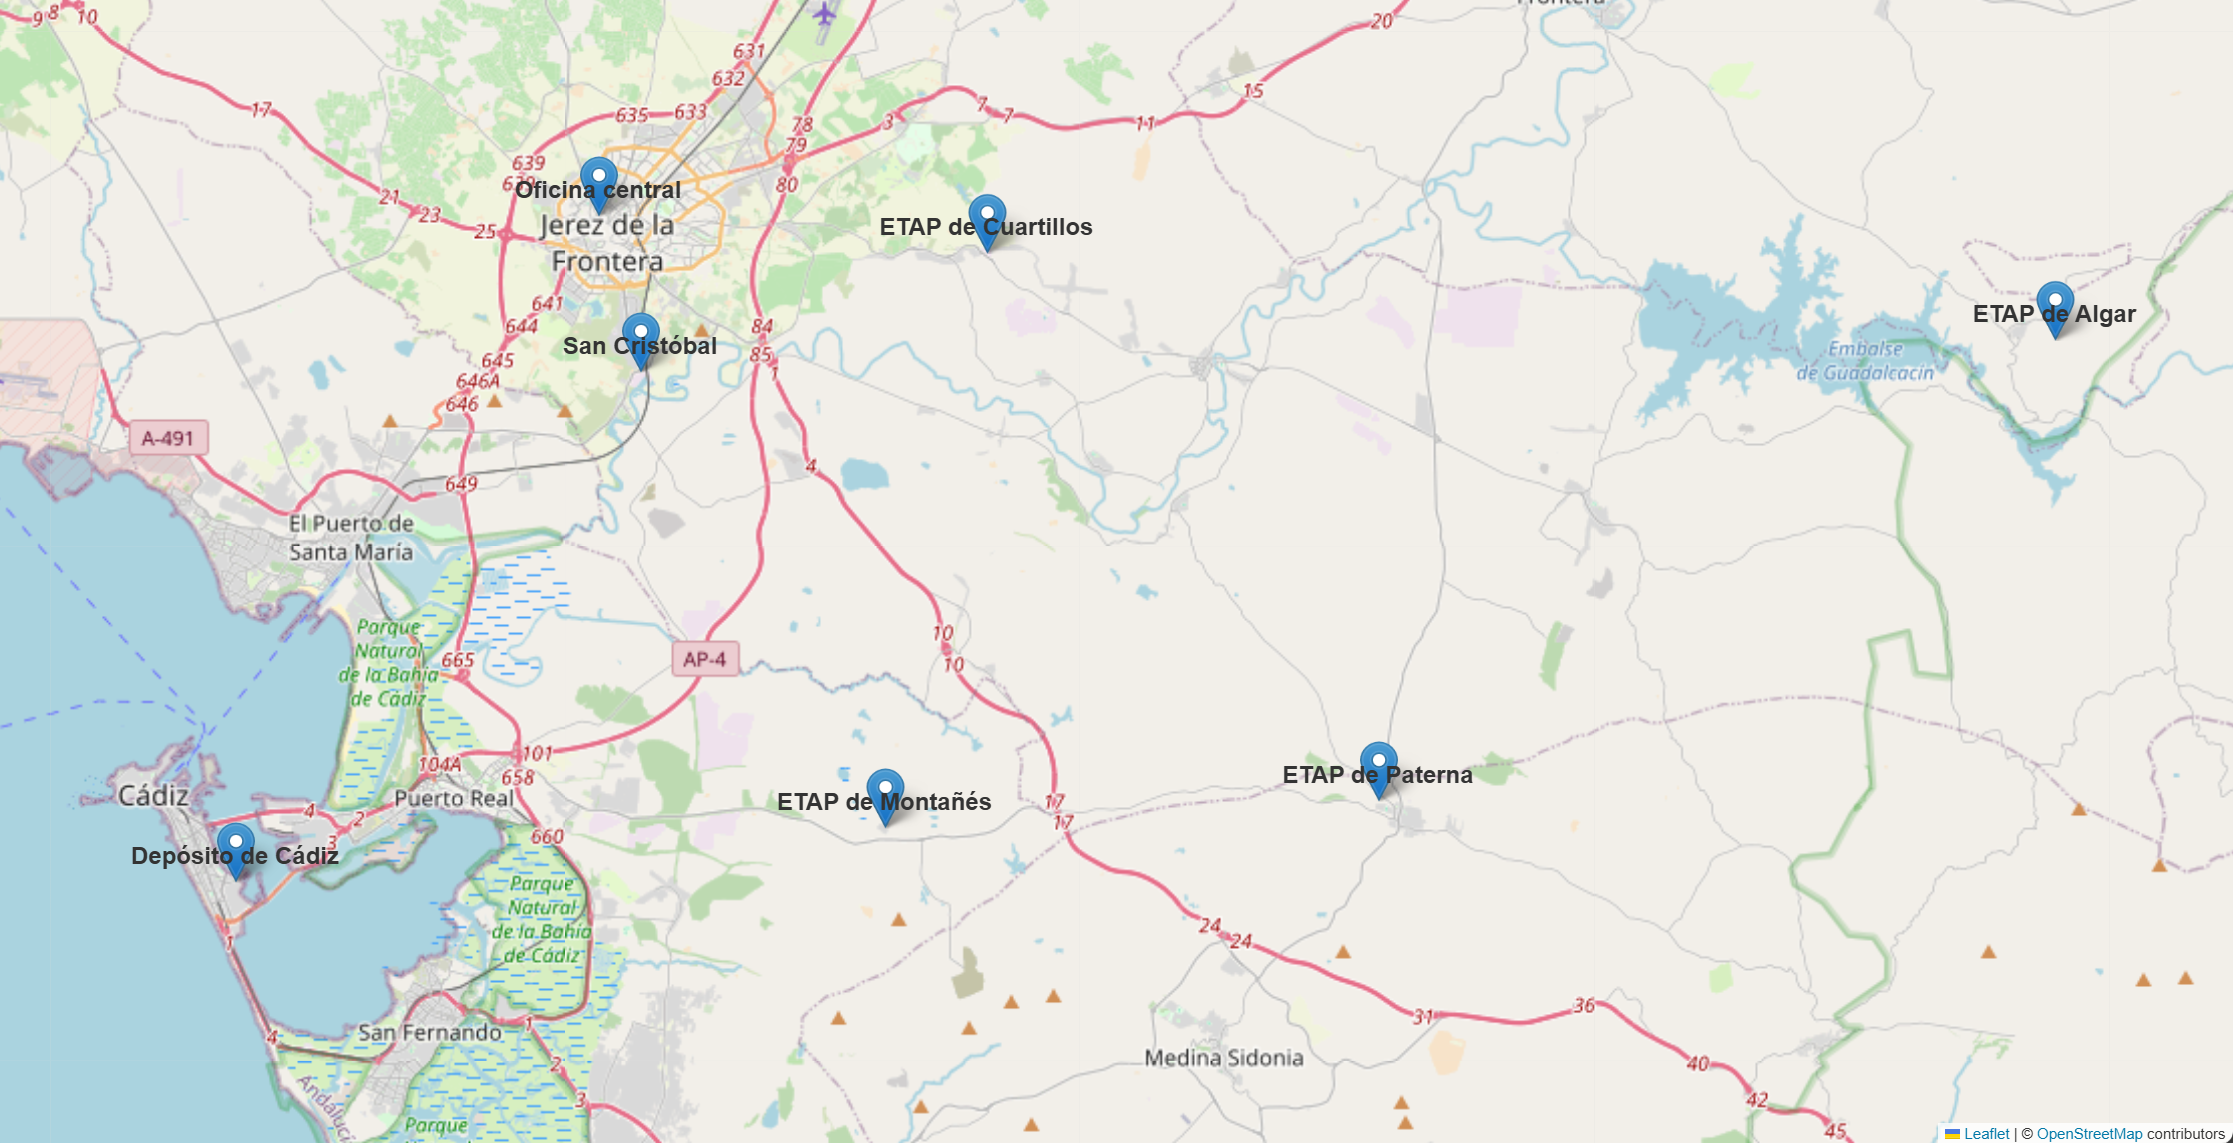
\includegraphics[width=0.95\textwidth]{images/mapa_sedes.png}
	\caption{Ubicación de las instalaciones}
	\label{fig:mapa_sedes}
\end{figure}

\subsection{SD-WAN (Software-Defined Wide Area Network)}
SD-WAN \cite{versa_sdwan} es una red de área extensa (WAN) que utiliza tecnología de redes definidas por software, ofreciendo servicios de red confiables y escalables. Esta tecnología permite simplificar el control y la administración de la infraestructura de red al proporcionar una arquitectura WAN virtual que conecta de manera segura a lo usuarios con las aplicaciones y servicios que necesitan. Asimismo, SD-WAN utiliza una combinación de tecnologías, como por ejemplo, MPLS, Internet de banda ancha y LTE, para ofrecer una conectividad flexible y de alto rendimiento. 

\vspace{0.5cm}
El funcionamiento de SD-WAN se basa en crear una superposición para virtualizar la red de área extensa, lo que permite un control centralizado, la simplificación de la administración y la implementación de los servicios de red.

\vspace{0.5cm}
\noindent
En cuanto a la arquitectura de este tecnología \cite{hpe_sdwan}, esta se compone de varios componentes clave, como:
\begin{itemize}
  \item \textbf{Dispositivos en el extremo:} son los dispositivos físicos o virtuales instalados en ubicaciones remotas, centro de datos y ubicaciones en la nube. Las cuales, tienen un rol importante como distribuir el tráfico según las políticas definidas y de medir en tiempo real el estado de la red.
  \item \textbf{Organizador de SD-WAN:} sirve para controlar las decisiones de política, como la gestión del tráfico y las rutas a utilizar.
  \item \textbf{Capa de transporte:} SD-WAN funciona con cualquier tecnología de transporte basado en IP, como MPLS, LTE, o 5G. Esta capa forma la red subyacente mientras que SD-WAN crea una red superpuesta inteligente con selección dinámica de rutas y conmutación de fallos. 
\end{itemize}

\subsection{MPLS (Multiprotocol Label Switching)}
\label{subsec:mpls}
MPLS (Multiprotocol Label Switching) \cite{wikipedia_mpls} es un mecanismo de transporte de datos que opera entre la capa de enlace de datos y la capa de red del modelo OSI. Este fue diseñado para unificar el servicio de circulación de datos para las redes basadas en circuitos y en paquetes. Asimismo, puede ser utilizado para transportar diferentes tipos de tráfico, incluyendo el de voz y el de paquetes IP.

\vspace{0.5cm}
\noindent
En una red MPLS existen diferentes elementos \cite{mpls_elements} que desempeñan distintas funciones en la red. En la Figura~\ref{fig:arquitectura_mpls} se puede observar una arquitectura de red MPLS típica.
\begin{enumerate}
  \item \textbf{Routers según ubicación y función en la red:}
  \begin{itemize}
    \item \textbf{Router del cliente (CE - Customer Edge):} es el router que se encuentra en el extremo del cliente. Puede ser cualquier router que se use para comunicarse con el proveedor de servicios.
    \item \textbf{Router de proveedor (PE - Provider Edge) o LER (Label Edge Router):} es el router frontera entre la red del cliente y la red MPLS del proveedor de servicios. Estos routers son los puntos de entrada y salida de la red MPLS.
    \item \textbf{Router troncal (P - Provider) o LSR (Label Switching Router):} es el router que se encarga de conmutar las etiquetas en el core de la red MPLS. Estos routers son responsables de dirigir el tráfico a través de la red utilizando las etiquetas asignadas. Además,
    intercambian estas etiquetas para dirigir el tráfico rápidamente a través de las red sin necesidad de analizar la dirección de destino de cada paquete. Su unión es puramente interno para el enrutamiento basado en etiquetas, por lo que no interactúan
    con los clientes.
  \end{itemize}
  \item \textbf{Otros elementos:}
  \begin{itemize}
    \item \textbf{LSP (Label Switched Path):} es el nombre genérico de un camino MPLS, es decir, es un túnel MPLS unidireccional establecido entre los extremos formado por un conjunto de LSRs.
    \item \textbf{LDP (Label Distribution Protocol):} es un protocolo para la distribución de etiquetas MPLS entre los equipos de la red.
    \item \textbf{FEC (Forwarding Equivalence Class):} es un grupo de paquetes tratados del mismo modo por el conmutador. Es decir, un conjunto de paquetes que se encaminan a través de la misma ruta en la red MPLS.
  \end{itemize}
\end{enumerate}

\begin{figure}[htb]
  \centering
  \includegraphics[width=1\textwidth]{images/Arquitectura_MPLS.png}
  \caption{Arquitectura MPLS}
  \label{fig:arquitectura_mpls}
\end{figure}

% MPLS se le conoce como un protocolo Layer 2.5, pues se encuentra entre la capa 2 (Enlace de datos) y la capa 3 (Red) del modelo OSI. Esto significa que MPLS puede trabajar con diferentes protocolos de red, como IP, Frame Relay y ATM, lo que lo hace muy versátil.

% \vspace{0.5cm}
%
% En la Figura~\ref{fig:mpls} se muestra una imagen de la cabecera de un paquete MPLS, que se compone de 4 campos, cada uno con un tamaño específico:
% La cabecera de un paquete MPLS se compone de 4 campos, cada uno con un tamaño específico:
% \begin{itemize}
%   \item \textbf{Label:} Es un campo de 20 bits que contiene la etiqueta de ruta utilizada para dirigir el paquete a su destino.
%   \item \textbf{CoS (Class of Service):} Es un campo de 3 bits que se utiliza para indicar la clase de servicio del paquete. Esto permite a los routers priorizar el tráfico según su importancia.
%   \item \textbf{S o BoS (Bottom of Stack):} Es un campo de 1 bit que se utiliza para indicar si la etiqueta es parte de una pila de etiquetas. 
%   \item \textbf{TTL (Time to Live):} Es un campo de 8 bits que se utiliza para indicar el tiempo de vida del paquete. Esto permite a los routers descartar paquetes que han estado en la red durante demasiado tiempo.
% \end{itemize}

% \begin{figure}[H]
%   \centering
%   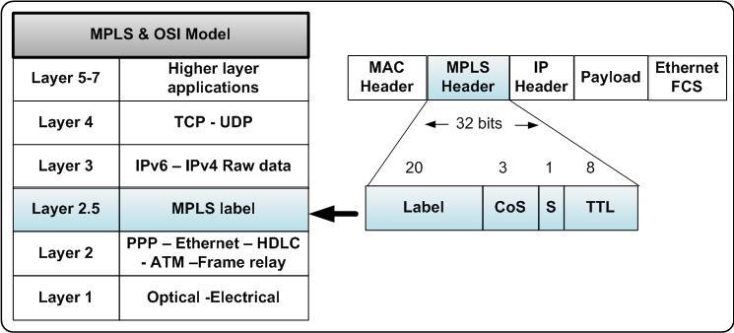
\includegraphics[width=0.9\textwidth]{images/MPLS-and-OSI-model.png}
%   \caption{Cabecera de MPLS, obtenida de \cite{mpls_elements}}
%   \label{fig:mpls}
% \end{figure}

\subsection{VPN (Virtual Private Network)}
\label{subsec:vpn}
Una VPN (Virtual Private Network) \cite{wikipedia_vpn} es una tecnología que garantiza una extensión segura de la red de área local (LAN) sobre Internet. Lo que permite establecer un enlace punto a punto con el uso de conexiones dedicadas, cifradas o la combinación de ambas. Existen diferentes arquitecturas VPN, cada una con sus propias características y casos de uso. A continuación, se describen las más comunes:

\begin{itemize}
  \item \textbf{VPN de acceso remoto:} permite a los usuarios conectarse a la red de la empresa desde ubicaciones remotas utilizando una conexión segura a través de Internet. Una vez conectados, tienen un nivel de acceso parecido al que tendrían en la red local de la empresa.
  \item \textbf{VPN punto a punto:} este esquema permite conectar dos redes remotas a través de Internet de forma segura, como si estuvieran en la misma red local.
  \item \textbf{VPN de sitio a sitio:} permite conectar múltiples redes remotas entre sí a través de Internet, creando una red privada virtual que conecta todas las sedes de la empresa.
  \item \textbf{VPN de extranet:} permite a socios comerciales o proveedores acceder de forma segura a recursos específicos de la red de la empresa.
\end{itemize}

\subsection{VoIP (Voice over IP)}
La tecnología VoIP \cite{voipstudio_que_es_voip} (Voice over IP) se refiere a la capacidad de realizar llamadas de voz a través de Internet en lugar de utilizar las líneas telefónicas tradicionales. Esencialmente, VoIP convierte las señales de voz en paquetes de datos que se transmiten a través de la red de Internet hasta llegar al destinatario, donde se convierten de nuevo en señales de voz.

\vspace{0.5cm}
VoIP ofrece varias ventajas sobre la telefonía tradicional, como costes más bajos en comparación con las tarifas de las líneas telefónicas convencionales, especialmente en llamadas de larga distancia e internacionales, e incluso suelen ser gratuitas o a un coste muy bajo. También, ofrece una mayor flexibilidad y escalabilidad, ya que permite añadir fácilmente líneas adicionales y funcionalidades avanzadas sin necesidad de instalar hardware adicional. Asimismo, permite la movilidad de los usuarios, ya que las llamadas pueden realizarse desde cualquier dispositivo con conexión a Internet.


\subsection{MP-BGP (Multiprotocol Border Gateway Protocol)}
MP-BGP (Multiprotocol Border Gateway Protocol) \cite{wikipedia_mp_bgp} es una extensión del protocolo BGP (Border Gateway Protocol) que permite distribuir en paralelo diferentes tipos de direcciones IP, como IPv4 e IPv6, además de, otros protocolos de red. Asimismo, utiliza una arquitectura básica con sistemas autónomos (AS) que se comunican a través de sesiones BGP e intercambian información de accesibilidad de red en forma de actualizaciones BGP \cite{linkedin_mp_bgp}. Estas se pueden clasificar en dos formas según el sistema autónomo (AS) al que pertenecen los routers que intercambian información de enrutamiento:

\begin{itemize}
  \item \textbf{iBGP (Internal BGP):} es la comunicación de routers del mismo sistema autónomo (AS) que intercambian información de enrutamiento.
  \item \textbf{eBGP (External BGP):} es la comunicación de routers de diferentes sistemas autónomos (AS) que intercambian información de enrutamiento.
\end{itemize}

Por otro lado, existen cuatro tipos de mensajes BGP \cite{wikipedia_bgp} que se utilizan para establecer y mantener las sesiones BGP:
\begin{itemize}
  \item \textbf{OPEN:} se utiliza para establecer una sesión BGP una vez haya sido establecido la conexión TCP.
  \item \textbf{UPDATE:} es un mensaje de actualización que contiene los anuncios de nuevos prefijos.
  \item \textbf{KEEPALIVE:} una vez la sesión BGP está activa, envía periódicamente un mensaje para mantener activa la conexión.
  \item \textbf{NOTIFICATION:} envía al cerrar una sesión BGP. Esto sucede cuando ocurre algún error.
\end{itemize}

\newpage

\section{Herramientas}
Las herramientas que se han utilizado para la realización de este proyecto son las siguientes:

\subsection{GNS3}
GNS3 (Graphic Network Simulator-3) \cite{gns3_wiki}, un simulador gráfico de red libre y de código
abierto que permite crear topologías de red complejas y poner en funcionamiento simulaciones sobre ellas, 
permitiendo así la combinación de dispositivos reales como virtuales.

\vspace{0.5cm}
Entre las principales características de GNS3 \cite{ccnadesdecero_gns3}, podemos destacar, que es un software gratuito y de código abierto, siendo disponible para Windows, Linux y macOS. De igual forma, no tiene límite en la cantidad de dispositivos que se pueden simular, a excepción de la limitación hardware: CPU y memoria. Además, permite la captura de paquetes de red con Wireshark, la conexión de redes simuladas con redes reales y está constantemente actualizado ya que cuenta con una comunidad de usuarios grande y activa (+800.000 usuarios).

\vspace{0.5cm}
Pero la ventaja principal es que los equipos de red simulados disponen de todas las funcionalidades de un equipo real, ya que ejecuta el mismo firmware que el equipo real. Permitiendo diseñar una topología de red simulada lo más parecida posible a una red real sin necesidad de tener los equipos físicos. 

\subsection{Wireshark}
Wireshark \cite{wikipedia_wireshark} es un analizador de protocolos utilizado para realizar análisis y solucionar problemas en redes de comunicaciones, para análisis de datos y protocolos, y como una herramienta didáctica.

\subsection{Docker}
Docker es \cite{docker_ubuntu_tutorial} una aplicación que simplifica el proceso de administración de procesos de software en contenedores. Estos permiten ejecutar aplicaciones en procesos con aislamiento de recursos. Son similares a las máquinas virtuales, pero son más portátiles, más flexibles con los recursos y más dependientes del sistema operativo host.

\subsection{VirtualBox}
Oracle VirtualBox \cite{virtualbox_introduction} es una herramienta de virtualización multiplataforma que permite ejecutar múltiples sistemas operativos simultáneamente en un mismo equipo físico, mediante la creación de máquinas virtuales (VM). Esta aplicación amplía las capacidades del sistema anfitrión, haciendo posible, por ejemplo, ejecutar distribuciones de Linux en un sistema Windows, o viceversa, así como combinar diferentes entornos como Windows 
y macOS o servidores Linux. 

\subsection{MicroSIP}
MicroSIP \cite{microsip} es un softphone de código abierto y portable, diseñado para sistemas operativos Windows y basado en la pila PJSIP. Esta herramienta permite realizar llamadas VoIP de alta calidad, tanto entre usuarios como hacia teléfonos convencionales, mediante el protocolo SIP (Session Initiation Protocol).

\subsection{Telefonos Grandstream GRP2601}
El teléfono Grandstream GRP2601 \cite{grandstream_grp2601_datasheet} es un modelo esencial de 2 líneas diseñado con aprovisionamiento zero-touch para implementación masiva y fácil gestión. Se caracteriza por tener un diseño elegante y un conjunto de funciones de última generación incluyendo conferencia de voz de 5 participantes para maximizar la productividad, soporte EHS para auriculares Plantronics, Jabra y Sennheiser y soporte en múltiples idiomas.

\subsection{Router Mikrotik RB2011UiAS-RM}
El router RB2011UiAS-RM \cite{mikrotik_rb2011uias_rm} de Mikrotik funciona con RouterOS, un sistema operativo de enrutamiento avanzado que ofrece funcionalidades como enrutamiento dinámico, hotspot, cortafuegos, MPLS, VPN, calidad de servicio, equilibrio de carga, supervisión en tiempo real y más. Este modelo destaca por sus cinco puertos LAN Gigabit, cinco puertos LAN Fast Ethernet, puerto serie RJ45, puerto USB, 128MB de RAM, licencia RouterOS L5 y pantalla LCD táctil para facilitar la configuración y gestión. 

\subsection{Switches TP-Link T2500G-10TS}
El T2500G-10TS \cite{tp_link_t2500g_10ts} es un switch gestionable con puertos Gigabit en todas sus interfaces, ideal para redes de alto rendimiento. Ofrece seguridad avanzada (IP-MAC-puerto, ACL, 802.1X, Radius, DoS, DHCP Snooping), QoS en L2/L3/L4 e IGMP Snooping para optimizar voz y video, y múltiples opciones de gestión (Web, CLI, Telnet, SSH, SNMP). Además, soporta funciones L2 como VLAN 802.1Q, QinQ, port mirroring y STP/RSTP/MSTP para una red estable y segura. 

%%%%%%%%%%%%%%%%%%%%%%%%%%%%%%%%%%%%%%%%%%%%%%%%%%%%%%%%%%%%%%%%%%%%%%%%%%%%%%%
\newpage{\pagestyle{empty}}
\thispagestyle{empty}

\chapter{\LARGE Análisis de requisitos y requerimientos}
\label{chapter:dos}

Como se indicó anteriormente no es objetivo implementar en la totalidad de las condiciones del pliego \cite{expediente0062020}. Aquí se detallan los aspectos más importantes que se van a considerar.

\section{Comunicaciones de datos e internet}
El proyecto contempla la provisión de servicios de transmisión de datos entre las distintas sedes del Consorcio y el acceso a Internet, estableciendo una red IP privada y asegurando su alineación con 
los principios de calidad, flexibilidad, fiabilidad, capacidad y tecnología avanzada. Los servicios de comunicación entre las sedes serán:
\begin{itemize}
	\item \textbf{Implementación de red IP privada:} se creará una red de datos utilizando circuitos dedicados para interconectar todas las sedes de manera segura, extendiendo y unificando las redes LAN existentes.
	\item \textbf{Acceso a Internet:} todas las sedes accederán a Internet a través del circuito ubicado en la Oficina Central. La totalidad de las sedes se conectarán a la red mediante la Intranet, utilizando un acceso único corporativo que estará soportado por fibra óptica, garantizando así una conexión eficiente y centralizada.
	\item \textbf{Escalabilidad y priorización de tráfico:} la red se diseñará para permitir un crecimiento futuro, garantizando el soporte para nuevos servicios y priorizando el tráfico, asegurando la calidad de la telefonía IP.
	\item \textbf{Tecnología de conexión:} se preferirá utilizar enlaces terrestres de fibra óptica, evitando tecnologías satelitales, con una obligación de mantener un alto nivel de disponibilidad en la configuración de la red.
	\item \textbf{Monitoreo y gestión:} elección de sistemas de monitorización en tiempo real que permitan la consulta del uso del caudal y alertas rápidas en caso de fallos.
	\item \textbf{Capacidades técnicas:} las conexiones deberán soportar una serie de requisitos de calidad del servicio (QoS), garantizando la baja latencia, alta capacidad de gestión de tráfico y compatibilidad con los estándares de direccionamiento de ITU-T.
\end{itemize}
\section{Servicio de electrónica de red gestionada}
\label{sec:servicio_electronica_red}
La infraestructura de red electrónica gestionada del Consorcio se diseñará para proporcionar una base sólida, flexible y escalable que permita el crecimiento y la adaptación a las necesidades cambiantes de la organización. 
Cada sede tendrá una red de área local (LAN) que garantice la conectividad eficiente de todos los dispositivos, asegurando la integración con la red IP privada y el resto de servicios corporativos.

\vspace{0.5cm}
Para ello, se instalarán switches gestionables que proporcionen la densidad de puertos Ethernet necesaria para conectar todos los equipos requeridos en cada sede, evitando el uso de hubs y asegurando una infraestructura moderna y eficiente. Estos switches soportarán velocidades mínimas de 100 Mbps por puerto y contarán con capacidades Power over Ethernet (PoE), lo que permitirá alimentar terminales VoIP y otros dispositivos de red directamente a través del cableado de datos, simplificando la instalación y el mantenimiento.

\vspace{0.5cm}
La solución de electrónica de red incluirá funcionalidades avanzadas como la configuración de VLANs para segmentar el tráfico, así como herramientas de Calidad de Servicio (QoS) que permitan clasificar y priorizar el tráfico, garantizando la calidad en servicios críticos como la telefonía IP. Además, se implementará la norma IEEE 802.3az para mejorar la eficiencia energética de la infraestructura.

\vspace{0.5cm}
En cuanto a la conectividad entre sedes, se proveerán routers de alto rendimiento que permitan la integración con tecnologías SD-WAN, facilitando la gestión centralizada y flexible de la red, así como el acceso seguro a través de conexiones VPN. Todo el equipamiento será seleccionado para asegurar la alta disponibilidad, la seguridad y la capacidad de adaptación a futuras ampliaciones o cambios en la red del consorcio.

\section{Servicio de seguridad gestionado}
\label{sec:servicios_seguridad_gestionado}
El servicio de seguridad gestionado se diseñará para proteger la infraestructura de red del consorcio, garantizando la confidencialidad, integridad y disponibilidad de los datos y servicios. Este servicio incluirá la elección de un cortafuegos de nueva generación (NGFW) que proporcionará una defensa robusta contra amenazas externas e internas, así como la gestión centralizada de la seguridad a través de un sistema de monitorización y gestión.

\vspace{0.5cm}
El consorcio dispondrá de un sistema de consulta estadística online para monitorizar y gestionar el uso del caudal mediante una aplicación web segura con autenticación de usuario. Además, dispondrá de un sistema de alertas en caso de que se produzca un fallo en los enlaces o en las líneas de acceso principales o de respaldo. También, el sistema de seguridad gestionado deberá incluir las siguientes características:
\begin{itemize}
	\item \textbf{Recepción de información:} el sistema permitirá la recepción de datos a través de SYSLOG para facilitar la monitorización continua y la identificación temprana de vulnerabilidades.
	\item \textbf{Actualizaciones y modificaciones:} se realizarán recomendaciones y actualizaciones remotas del software en caso de detectar vulnerabilidades, así como modificaciones en políticas de seguridad como respuesta a incidentes.
	\item \textbf{Centro de gestión:} habrá un centro de gestión en las instalaciones del licitador, que operará de manera coordinada y homogénea con el Consorcio.
\end{itemize}

Por otro lado, se elegirá una plataforma de seguridad avanzada para la gestión de amenazas que limite el tráfico entre Internet y la red interna del Consorcio, proporcionando funcionalidades como filtrado antivirus, detección de aplicaciones, control de navegación y respuesta ante incidentes. Además, se combinará con un sistema de respuesta ante incidentes que automatice procedimientos predefinidos y gestione accesos mediante VPN, garantizando una solución rápida y efectiva ante eventos de seguridad.

\subsection{Especificaciones técnicas del equipamiento}
\label{subsec:especificaciones_tecnicas_firewall}
\noindent
El cortafuegos debe cumplir con las siguientes especificaciones:
\begin{itemize}
  \item \textbf{Certificaciones:} ICSA, NSS Labs y Common Criteria.
  \item \textbf{Rendimiento:} hasta 20/20/9 Gbps de firewall, 2 millones de sesiones concurrentes, 135.000 nuevas sesiones por segundo, y 1.2 Gbps de Threat Protection.
  \item \textbf{Funcionalidades:} IPS (hasta 6 Gbps), proxy explícito, visualización de tráfico, escaneo de vulnerabilidades, antivirus, antispam y filtrado de contenidos.
  \item \textbf{Licenciamiento:} por equipo, no por usuario.
  \item \textbf{Interfaces:} 14 puertos 1GE RJ45 internos, 2 puertos WAN, 2 slots SFP, 2 puertos Management/DMZ, 2 para HA, 1 consola y 1 USB.
  \item \textbf{Virtualización:} soporte de 10 dominios virtuales con monitorización de recursos.
  \item \textbf{Control de aplicaciones:} identificación de 2900+ aplicaciones, clasificación granular y detección bajo túneles HTTPS.
  \item \textbf{Visibilidad:} consolidación de logs, visualización en tiempo real y gestión de sesiones.
  \item \textbf{Filtrado de contenidos:} control granular de URLs, cuotas de tiempo, listas blancas/negras, filtrado DNS y sinkhole.
  \item \textbf{Seguridad:} políticas por interfaz, prevención de amenazas, DLP, actualizaciones automáticas, doble factor de autenticación, bloqueo de botnets, inspección SSL y motor WAF.
  \item \textbf{VPN:} hasta 9 Gbps IPSec, 300 usuarios VPN SSL simultáneos, soporte para múltiples protocolos VPN.
\end{itemize}

\section{Comunicaciones fijas de voz}
En este apartado se detallan alguno de los requisitos que debe cumplir el servicio de comunicaciones fijas de voz, aunque no se contempla su implementación en el alcance de este proyecto. Estos requisitos servirán como referencia para futuras fase.

\vspace{0.5cm}
\noindent
Las especificaciones requeridas incluyen:
\begin{itemize}
	\item \textbf{Integración y escalabilidad:} se contempla al menos 38 extensiones, renovando los terminales actuales por modelos de VoIP.
	\item \textbf{Requisitos técnicos:} la centralita estará alojada preferentemente en la nube, con los terminales IP instalados localmente en cada sede. Se utilizarán conexiones IP estándar para la gestión de llamadas, permitiendo una numeración integrada y acceso a diferentes tipos de terminales, incluidos modelos de sobremesa.
	\item \textbf{Funcionalidades avanzadas:} se requerirán características como buzones de voz, grabación de llamadas y operadora automática personalizada. Se definirán grupos de salto y captura para optimizar el manejo de las llamadas.
	\item \textbf{Cableado y accesibilidad:} se deberá contemplar el cableado de datos de categoría CAT6, asegurando la conectividad necesaria para la telefonía IP y los servicios de datos, así como la posibilidad de adaptación a futuras necesidades en infraestructura.
	\item \textbf{Gestión y mantenimiento:} se exigirá la operación y mantenimiento integral de la red durante el contrato, garantizando la gestión continua y la evolución de los servicios conforme avance la tecnología.
\end{itemize}

\label{sec:requisitos_telefonia_ip}
\vspace{0.3cm}
Asimismo, los teléfonos IP que se utilicen deberán cumplir, como mínimo, los siguientes requisitos:
\begin{itemize}
	\item Dos puertos Ethernet de 100Mbps o de 1Gbps: uno para la alimentación y conexión a la red del terminal y otro para la conexión del PC al terminal, permitiendo la alimentación tanto por red eléctrica como a través del puerto Ethernet (PoE, Power over Ethernet).
	\item Disponer de manos libres full dúplex con altavoz y micrófono ambiente. Los terminales deberán ser completamente nuevos.
	\item Permitir la asignación de dirección IP mediante DHCP.
\end{itemize}

%%%%%%%%%%%%%%%%%%%%%%%%%%%%%%%%%%%%%%%%%%%%%%%%%%%%%%%%%%%%%%%%%%%%%%%%%%%%%%%
\newpage{\pagestyle{empty}}
\thispagestyle{empty}

\chapter{\LARGE Diseño}
\label{chapter:tres}

En este capítulo se describirá el diseño de la red de la empresa, incluyendo la topología,
la infraestructura de red, los dispositivos de red que se van a utilizar y las tecnologías implementadas.

\section{Diseño de red}
Para interconectar las sedes de la empresa se ha optado por una topología en estrella
porque se centraliza la gestión en un nodo central (oficina central). Además, el pliego de proyectos \footnote{\href{https://contrataciondelestado.es/wps/wcm/connect/PLACE_es/Site/area/docAccCmpnt?srv=cmpnt&cmpntname=GetDocumentsById&source=library&DocumentIdParam=10e9102e-09a6-42de-810d-d08c7c77bd65}{\texttt{Pliego de prescripciones técnicas para la contratación de servicios de telecomunicaciones de voz, fijas y móviles, red de acceso de datos,
			intranet e internet para el Consorcio de Aguas de la Zona Gaditana}}} especifica que \textit{``accederán a internet através del circuito ubicado al efecto en la Sede Principal''}, por lo que el acceso a Internet será unicamente en este punto, simplificando así la administración y el mantenimiento de la red. Además, permite que sea escalable, ya que se pueden agregar más edificios sin tener que reconfigurar toda la red. Esta estructura facilita redundancia en el núcleo y reduce costos al evitar conexiones complejas. En la Figura~\ref{fig:interconexion} se puede observar una representación gráfica de la topología en estrella de las instalaciones de la empresa.

\vspace{0.5cm}
Como tecnología principal de interconexión entre las sedes se ha optado por SD-WAN (Software Defined Wide Area Network) ya que permite una gestión centralizada, mayor flexibilidad, seguridad avanzada y facilita la integración de múltiples sedes e integración en tiempo real sin interrupciones. Esta tecnología es ideal para empresas que necesitan conectar varias ubicaciones de manera eficiente, segura y con capacidad de adaptación a diferentes proveedores y tipos de acceso.
Además, permite priorizar el tráfico crítico, aplicar políticas de seguridad de forma centralizada y simplificar
la administración de la red.

\vspace{0.5cm}
Para la interconexión de las sedes se han estudiado varios proveedores de servicios de telecomunicaciones, como Vodafone, Orange y Telefónica. Para este proyecto se ha optado por Vodafone como principal operador por su mejor oferta de servicios, precios y por ajustarse a las necesidades de la red. Vodafone ofrece un servicio de SD-WAN de Cisco Meraki que permite la creación de redes privadas virtuales (VPN), proporciona una mayor seguridad y control sobre el tráfico de datos, y facilita la gestión centralizada de la red. En la Tabla~\ref{tab:proveedores_red} se puede observar los proveedores de servicios de telecomunicaciones estudiados y las características principales de cada uno.

\begin{figure}[H]
	\centering
	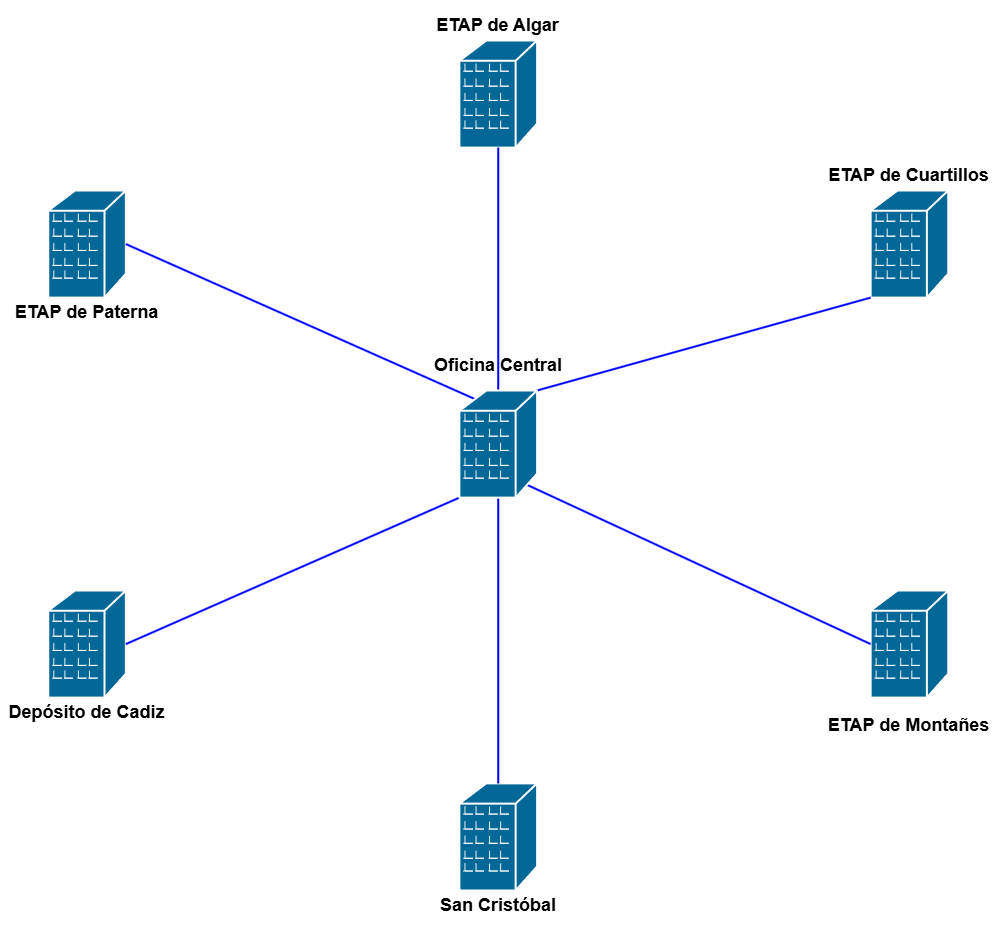
\includegraphics[width=0.7\textwidth]{images/Esquema_interconexion_sedes.png}
	\caption{Esquema de interconexión de sedes}
	\label{fig:interconexion}
\end{figure}

\begin{table}[htb]
	\centering
	\resizebox{\textwidth}{!}{%
		\begin{scriptsize}
			\begin{tabular}{|l|p{2.8cm}|p{3.3cm}|p{4cm}|c|}
				\hline
				\textbf{Proveedor} & \textbf{Tecnología principal} & \textbf{Seguridad y gestión}                                   & \textbf{Ventajas destacadas}                                               & \textbf{Precio/mes/sede}         \\
				                   &                               &                                                                &                                                                            & \footnotesize{(IVA no incluido)} \\ \hline
				Orange             & VPN, FTTH                     & Soluciones de seguridad integrales en la nube.                 & Red privada y unificada, acceso sencillo a recursos compartidos.           & 50\,€                            \\ \hline
				Telefónica         & SD-WAN (Cisco Meraki), MPLS   & Firewall avanzado y control de accesos, detección de amenazas. & Integración con Cisco Meraki y gestión centralizada sin inversión inicial. & 75\,€                            \\ \hline
				Vodafone           & SD-WAN (Cisco Meraki), VPN    & Firewall de última generación y gestión centralizada.          & Visualización avanzada del tráfico y conectividad mejorada entre sedes.    & 64\,€                            \\ \hline
			\end{tabular}
		\end{scriptsize}
	}
	\caption{Comparativa de proveedores de servicios de telecomunicaciones}
	\label{tab:proveedores_red}
\end{table}

Por otro lado, se pide para algunas sedes (no se especifica cuáles), un caudal de respaldo obligatorio que tiene que ir montado sobre distinta infraestructura o aplicando tecnologías diferentes o distinto operador. Para ello, se va a optar por Telefónica utilizando también su servicio SD-WAN de Cisco Meraki. Además, se pide que se tenga un un dispositivo independiente y distinto al principal para el enlace de respaldo, para esto, contará con un dispositivo diferente configurado en modo \textit{Warm Spare (HA)} \cite{meraki_warm_spare}, lo que garantiza la continuidad del servicio mediante un segundo equipo en espera, preparado para asumir el control en caso de que el principal falle. También, la funcionalidad de SD-WAN inteligente de Meraki permitirá balancear el tráfico entre el enlace principal y el enlace de respaldo (en este caso, la solución flexWAN de Telefónica), seleccionando dinámicamente el mejor camino según la calidad del enlace y las políticas definidas, asegurando así la redundancia de red y alta disponibilidad

\subsection{Diseño estructural}
La arquitectura de red se ha diseñado siguiendo un modelo jerárquico de tres capas: núcleo, distribución y acceso. Esta jerarquía permite una mejor gestión del tráfico, escalabilidad y redundancia en la red.
\begin{itemize}
	\item \textbf{Capa de núcleo:} se encarga de la interconexión entre las diferentes sedes y la oficina central. Se utilizan dispositivos de alto rendimiento para garantizar una alta disponibilidad y baja latencia en la comunicación entre sedes.
	\item \textbf{Capa de distribución:} se encuentran los dispositivos que conectan los diferentes segmentos de la red, como switches y routers. Se encargan de la gestión del tráfico y la seguridad de la red.
	\item \textbf{Capa de acceso:} se conectan los hosts finales, como ordenadores, impresoras y teléfonos IP. Se utilizan switches de acceso para conectarlos a la red.
\end{itemize}

En la Figura~\ref{fig:diseño_vertical_red} se puede observar el cableado vertical de alguna de las sedes de la empresa.
Esta se encarga de conectar las diferentes plantas de un edificio, permitiendo la interconexión entre los armarios de comunicaciones de cada piso y asegurando la continuidad de la red a lo largo de toda la estructura vertical del edificio. ETAP Cuartillos y ETAP Montañés tienen una organización similar entre ellas y, por otro lado, ETAP Paterna, ETAP Algar y el Depósito de Cádiz comparten una configuración parecida entre sí. La oficina central presenta una estructura diferente al resto, ya que alberga los diferentes servidores de la empresa y la DMZ (zona desmilitarizada) donde se alojan los servidores de la empresa.

\begin{figure}[H]
	\centering
	\includegraphics[width=1\textwidth]{images/diseño_vertical_sedes.png}
	\caption{Diseño vertical de la red}
	\label{fig:diseño_vertical_red}
\end{figure}

En el esquema de red de la Figura~\ref{fig:diseño_vertical_red}, las líneas rojas indican el núcleo de la infraestructura, donde se ubican los dispositivos core y de distribución que manejan el tráfico principal entre sedes. Las líneas naranjas corresponden a la zona de distribución, conectando los equipos de distribución con los de acceso. Por su parte, las líneas amarillas representan la capa de acceso, donde se integran los dispositivos finales. Los círculos en tonos celeste pastel y lila identifican las VLAN de datos y voz, respectivamente, mientras que en la oficina central, el área marcada con un recuadro amarillo indica la DMZ, donde se alojan los servidores corporativos. Para el cableado, se empleará fibra óptica monomodo en los enlaces principales entre los equipos de core y distribución, así como en los tramos verticales entre plantas, garantizando así alta velocidad y baja latencia. En la capa de acceso y para la conexión de los equipos finales, se utilizará cableado estructurado de cobre categoría 6A (Cat 6A), adecuado para velocidades de hasta 10 Gbps dentro de edificios.

\vspace{0.5cm}
En la Figura~\ref{fig:diseño_general} se puede observar el diseño general de la red de la empresa, donde se muestra la interconexión entre las diferentes sedes y la oficina central. Este diseño general permite visualizar cómo se conectan todas las instalaciones de la empresa, formando una red corporativa unificada que facilita la gestión centralizada y la comunicación entre todas las sedes.

\begin{figure}[htb]
	\centering
	\includegraphics[width=1\textwidth]{images/diseño_general.png}
	\caption{Diseño representativo de la red de la empresa}
	\label{fig:diseño_general}
\end{figure}

\subsection{Dispositivos de red}
\label{subsubsec:dispositivos_red}
En esta sección se detallan los equipos de red elegidos para poner en marcha la infraestructura de comunicaciones de
a empresa. Aunque Vodafone no especifica detalladamente los modelos que se entrega a sus clientes, sí se especifica que su solución SD-WAN está basada en la tecnología Cisco Meraki.

% Aunque algunos dispositivos, como los routers o firewalls, suelen ser facilitados por el proveedor de
% telecomunicaciones, en este caso no se cuenta con información precisa sobre los modelos que serán entregados. Por ello,
% se ha optado por seleccionar ejemplos representativos que cumplen con las características técnicas y operativas
% requeridas para el diseño planteado.

% \subsubsection{Dispositivos SW-WAN (Cisco Meraki)}
% Como Vodafone como trabaja con la tecnología SD-WAN de Cisco Meraki se ha optado por realizar una estimación técnica realista de los dispositivos que se usaran. En este caso, se usara equipamiento UTM (Unified Threat Management) que es aquel que tiene múltiples funciones como firewall, VPN, detección de intrusiones y filtrado de contenido. Estos dispositivos proporcionan una solución integral para la seguridad de la red y son ideales para empresas que buscan simplificar su infraestructura de seguridad. 

\subsubsection{Dispositivos de interconexión}
Dado que el proveedor de servicios elegido es Vodafone, el cual ofrece soluciones de conectividad basadas en la tecnología SD-WAN de Cisco Meraki, se ha optado por realizar una estimación técnica realista de los dispositivos que podrían instalarse en cada sede.

\newpage

\vspace{0.5cm}
En este proyecto se propone el uso de dispositivos de la gama Cisco Meraki MX, los cuales son \textit{appliances} de red de tipo UTM (Unified Threat Management). Estos dispositivos combinan en un solo equipo funciones avanzadas de enrutamiento, cortafuegos de nueva generación, conectividad VPN automática (AutoVPN), detección y prevención de intrusiones (IDS/IPS), así como filtrado de contenido.

% \vspace{0.5cm}
%
% Su integración en la arquitectura SD-WAN permite una gestión centralizada desde la nube (Meraki Dashboard), así como la aplicación de políticas de red, seguridad y calidad de servicio de forma unificada. Este tipo de equipamiento resulta especialmente adecuado para entornos distribuidos como el de este proyecto, ya que permite simplificar la infraestructura, mejorar la seguridad y facilitar la escalabilidad de la red.

\vspace{0.5cm}
En la Tabla~\ref{tab:justificacion_meraki} se presenta una justificación técnica de los dispositivos Cisco Meraki MX~\footnote{\href{https://meraki.cisco.com/lib/pdf/meraki_datasheet_mx_es.pdf}{\texttt{Ficha técnica de los Meraki MX}}} propuestos para cada sede del Consorcio de Aguas de la Zona Gaditana. Se ha seleccionado un modelo específico para cada sede, teniendo en cuenta el tamaño y las necesidades de conectividad de cada una.

\begin{table}[H]
	\centering
	\resizebox{\textwidth}{!}{%
		\begin{scriptsize}
			\begin{tabular}{|c|c|p{6cm}|c|}
				\hline
				\textbf{Sede}   & \textbf{Modelo propuesto} & \textbf{Justificación}                                                                                                                                                                                                                                                                              & \textbf{Precio estimado (€)} \\ \hline
				Oficina Central & MX95                      & Nodo central de la red SD-WAN. Actúa como concentrador VPN y punto de salida único a Internet. Requiere alto rendimiento y escalabilidad.                                                                                                                                                           & 3.700                        \\ \cline{2-4}
				                & MX85                      & Será el dispositivo secundario (redundancia) que estará preparado (Warm Spare) en caso de que el principal falle.                                                                                                                                                                                   & 2.130                        \\ \hline
				San Cristóbal   & MX68                      & Sede mediana. El modelo permite hasta 50 usuarios y ofrece margen de crecimiento. Adecuado para cargas medias y conexiones VPN estables.                                                                                                                                                            & 650                          \\ \hline
				\multirow{5}{*}{\begin{tabular}[c]{@{}c@{}}ETAP de Cuartillos\\ ETAP de Montañés\\ ETAP de Paterna\\ ETAP de Algar\\ Depósito de Cádiz\end{tabular}}
				                & \multirow{5}{*}{MX67}     & Sedes pequeñas con necesidades similares de conectividad y escalabilidad. El modelo MX67 es compacto, económico y soporta hasta 50 usuarios, ofreciendo suficientes puertos LAN y funcionalidades para entornos de bajo o moderado tráfico, manteniendo un buen balance entre coste y prestaciones. & \multirow{5}{*}{420}         \\ \hline
			\end{tabular}
		\end{scriptsize}
	}
	\caption{Justificación técnica de los dispositivos Cisco Meraki MX por sede}
	\label{tab:justificacion_meraki}
\end{table}

\noindent
Los modelos seleccionados de la serie Meraki MX  ofrecen las siguientes características:
\begin{itemize}
	\item \textbf{Rendimiento y escalabilidad:} estos modelos están diseñados para manejar cargas de trabajo medianas a altas, con capacidades de procesamiento y memoria adecuadas para soportar múltiples conexiones VPN y tráfico de red.
	\item \textbf{Seguridad avanzada:} todos los modelos incluyen funcionalidades de seguridad integradas, como firewall de nueva generación, detección y prevención de intrusiones (IDS/IPS), filtrado de contenido y protección contra malware, lo que garantiza una defensa robusta contra amenazas cibernéticas.
	\item \textbf{Conectividad VPN:} establecen automáticamente túneles VPN sitio a sitio con conectividad con IPsec
	\item \textbf{Gestión centralizada:} todos los dispositivos se gestionan a través del Meraki Dashboard, que es una plataforma en la nube de Meraki que permite la administración centralizada de la red, la monitorización del rendimiento y la aplicación de políticas de seguridad y calidad de servicio de forma unificada.
	\item \textbf{Facilidad de implementación:} los dispositivos Meraki son conocidos por su facilidad de instalación y configuración, lo que reduce el tiempo y los recursos necesarios para poner en marcha la red.
\end{itemize}

\subsubsection{Switches}
El Consorcio de Aguas de la Zona Gaditana cuenta con siete sedes distribuidas por la provincia de Cádiz.
En la Tabla~\ref{tab:sedes_puertos_acceso} se detalla el número mínimo de puntos de acceso requeridos
para cada sede. Considerando que cada trabajador necesita un ordenador y un teléfono IP, se ha
duplicado el número de puertos solicitados. Además, se ha implementado un margen de crecimiento
del 20\% para permitir futuras ampliaciones de la infraestructura de red.

\begin{table}[H]
	\centering
	\small
	\begin{tabular}{|l|l|l|l|l|}
		\hline
		\textbf{Denominación de la sede} & \textbf{Nº de puertos mínimo} & \textbf{Nº de puertos con escalabilidad} \\ \hline
		Oficina central                  & 30                            & 72                                       \\ \hline
		San Cristóbal                    & 15 + 5 + 5                    & 36 + 12 + 12                             \\ \hline
		ETAP de Cuartillos               & 5 + 5                         & 12 + 12                                  \\ \hline
		ETAP de Montañés                 & 5 + 5                         & 12 + 12                                  \\ \hline
		ETAP de Paterna                  & 5                             & 12                                       \\ \hline
		ETAP de Algar                    & 5                             & 12                                       \\ \hline
		Depósito de Cádiz                & 5                             & 12                                       \\ \hline
	\end{tabular}
	\caption{Número de puertos de acceso a la red}
	\label{tab:sedes_puertos_acceso}
\end{table}

Se han comparado diferentes modelos de switches por fabricante según las necesidades de cada sede (ver Tabla~\ref{tab:switches}). Finalmente, se seleccionan dispositivos Cisco por su relación calidad-precio: el Catalyst 9300-24P \cite{cisco_9300_24p_e_shop, cisco_9300_24p_e_datasheet} para la Oficina Central y San Cristóbal, el Catalyst 3560-CX-12PD-S \cite{cisco_3560_cx_12pd_s_shop, cisco_3560_cx_12pd_s_datasheet} para el resto de sedes, y el WS-C2960L-16TS-LL \cite{cisco_2960l_16ts_ll_datasheet} como switch de acceso en todos los edificios.

\renewcommand{\arraystretch}{1.2} % Puedes ajustar el valor (1.2, 1.3, 1.5, etc.). Esto es para aumentar el espacio entre filas
\begin{table}[H]
	\centering
	\small
	\resizebox{\textwidth}{!}{%
		\begin{tabular}{|c|c|c|c|c|}
			\hline
			\textbf{Fabricante} & \textbf{Rol} & \textbf{Modelo}         & \textbf{Sedes que lo necesitan}          & \textbf{Precio/unidad} \\ \hline
			Cisco               & Distribución & Catalyst 9300-24P       & Oficina Central, San Cristóbal           & 1.160€                 \\ \cline{3-5}
			                    &              & Catalyst 3560-CX-12PD-S & ETAP Cuartillos, ETAP Montañés,          & 1.120€                 \\
			                    &              &                         & ETAP Paterna, ETAP Algar, Depósito Cádiz &                        \\ \cline{2-5}
			                    & Acceso       & WS-C2960L-16TS-LL       & Oficina Central (5), San Cristóbal (4)   & 410€                   \\
			                    &              &                         & ETAP Cuartillos (2), ETAP Montañés (2)   &                        \\
			                    &              &                         & ETAP Paterna, ETAP Algar, Depósito Cádiz &                        \\ \hline

			Juniper             & Distribución & EX4300-24P              & Oficina Central, San Cristóbal           & 2.900€                 \\ \cline{3-5}
			                    &              & EX2300-C-12P            & ETAP Cuartillos, ETAP Montañés,          & 700€                   \\
			                    &              &                         & ETAP Paterna, ETAP Algar, Depósito Cádiz &                        \\ \cline{2-5}
			                    & Acceso       & EX2300-C-12P            & Oficina Central (6), San Cristóbal (5)   & 700€                   \\
			                    &              &                         & ETAP Cuartillos (2), ETAP Montañés (2),  &                        \\
			                    &              &                         & ETAP Paterna, ETAP Algar, Depósito Cádiz &                        \\ \hline

			Huawei              & Distribución & S5720-28X-PWR-SI-AC     & Oficina Central, San Cristóbal           & 1.030€                 \\ \cline{3-5}
			                    &              & S5720-14X-PWH-SI-AC     & ETAP Cuartillos, ETAP Montañés,          & 700€                   \\
			                    &              &                         & ETAP Paterna, ETAP Algar, Depósito Cádiz &                        \\ \cline{2-5}
			                    & Acceso       & S5720-28X-PWR-LI-AC     & Oficina Central (3), San Cristóbal (4)   & 360€                   \\
			                    &              &                         & ETAP Cuartillos (2), ETAP Montañés (2),  &                        \\
			                    &              &                         & ETAP Paterna, ETAP Algar, Depósito Cádiz &                        \\ \hline
		\end{tabular}%
	}
	\caption{Comparativa de switches por fabricante y sedes según necesidades.}
	\begin{tcolorbox}[colback=gray!10!white, colframe=gray!70!black, title=NOTA:, size=title]
		\textit{El número reflejado en cada paréntesis indica la cantidad de dispositivos de ese tipo en las sedes mencionadas}
	\end{tcolorbox}
	\label{tab:switches}
\end{table}
\renewcommand{\arraystretch}{1} % Restablecer el valor por defecto

\subsubsection{Firewall}
Siguiendo las especificaciones técnicas descritas en la sección~\ref{subsec:especificaciones_tecnicas_firewall}, y teniendo en cuenta que Vodafone trabaja con dispositivos de la marca Fortinet, se ha seleccionado el modelo \texttt{Fortinet FortiGate FG-100F-HA} como solución de seguridad perimetral para la sede central.

\vspace{0.5cm}
Este firewall de próxima generación proporciona un conjunto completo de funcionalidades de protección, incluyendo prevención de intrusiones, inspección profunda de paquetes (DPI), control de aplicaciones, filtrado web y antivirus. Su integración permite reforzar la seguridad del perímetro WAN y complementar las funciones básicas de firewall ya incluidas en los dispositivos Cisco Meraki MX utilizados en la red SD-WAN.

\vspace{0.5cm}
El modelo FG-100F-HA permite configuraciones en alta disponibilidad (HA), soporta múltiples interfaces de red de alta velocidad y está diseñado para entornos empresariales de tráfico medio-alto, como es el caso de la oficina central que actúa como nodo concentrador del tráfico de todas las sedes.

\vspace{0.5cm}
Esta solución permite reforzar la seguridad global de la red, especialmente en el punto crítico donde se concentra todo el tráfico proveniente de las sedes remotas. El FortiGate actúa como firewall perimetral, mientras que el \textit{appliance} Cisco Meraki MX250 se encarga de la conectividad SD-WAN, aunque tiene firewall integrado pero no suficiente para esta red de la empresa, estos se complementan entre sí para proporcionar una solución de seguridad robusta y escalable.

\subsubsection{Telefonía IP}
En cuanto a la telefonía IP, se ha optado por teléfonos que cumplan con los requisitos que se comentan en la sección \ref{sec:requisitos_telefonia_ip}. En la Tabla~\ref{tab:telefonos_ip} se muestran algunos modelos que cumplen con los requisitos necesarios que pide el pliego de proyectos.
\begin{table}[H]
	\centering
	\small
	\begin{tabular}{|c|c|c|p{6.5cm}|}
		\hline
		\textbf{Fabricante} & \textbf{Modelo} & \textbf{Precio aprox.} & \textbf{Características principales}                                                                                                               \\ \hline
		Grandstream         & GRP2602G        & 37€                    & 2 lineas y 4 cuentas SIP, puertos Gigabit con PoE integrado, pantalla LCD, manos libres Full-Duplex, audio HD, EHS                                 \\ \hline
		Grandstream         & GRP2612G        & 45€                    & 4 lineas multiuso y 4 cuentas SIP, dobles puertos GE a 10/100/1000 Mbps con PoE integrada, audio HD (Noise Shield), Wi-Fi de doble banda integrado \\ \hline
		Yealink             & SIP-T31G        & 55€                    & 2 cuentas VoIP, pantalla LCD, doble puerto Gigabit Ethernet, manos libre Full-Duplex, soporte IPv6, EHS                                            \\ \hline
		Fanvil              & X3SP Pro        & 65€                    & 4 líneas SIP, Auriculares inalámbricos EHS, Puertos rápidos duales, PoE integrado, Full-Duplex (AEC)                                               \\ \hline
	\end{tabular}
	\caption{Comparativa de Teléfonos IP}
	\label{tab:telefonos_ip}
\end{table}

Se va a optar por el modelo \texttt{Grandstream GRP2612G} \cite{grandstream_grp2612_datasheet} para toda la empresa, ya que es un modelo que cumple con los requisitos técnicos necesarios y es compatible con la solución de telefonía en la nube.

\subsubsection{Resumen de los dispositivos de red}
En la Tabla~\ref{tab:dispositivos_red} se presenta un resumen de los dispositivos de red seleccionados para el Consorcio de Aguas de la Zona Gaditana.

\begin{table}[H]
	\centering
	\small
	\resizebox{\textwidth}{!}{%
		\begin{tabular}{|c|c|c|c|c|}
			\hline
			\textbf{Dispositivo}                          & \textbf{Modelo}         & \textbf{Cantidad} & \textbf{Precio/unidad} & \textbf{Precio total} \\ \hline
			Dispositivo SD-WAN                            & Cisco Meraki MX95       & 1                 & 3.700€                 & 3.700€                \\ \hline
			Dispositivo SD-WAN                            & Cisco Meraki MX85       & 1                 & 2.130€                 & 2.130€                \\ \hline
			Dispositivo SD-WAN                            & Cisco Meraki MX68       & 1                 & 650€                   & 650€                  \\ \hline
			Dispositivo SD-WAN                            & Cisco Meraki MX67       & 5                 & 420€                   & 2.100€                \\ \hline
			Switch de distribución                        & Catalyst 9300-24P       & 2                 & 1.160€                 & 2.320€                \\ \hline
			Switch de distribución                        & Catalyst 3560-CX-12PD-S & 5                 & 1.120€                 & 5.600€                \\ \hline
			Switch de acceso                              & WS-C2960L-16TS-LL       & 16                & 410€                   & 6.560€                \\ \hline
			Firewall                                      & FortiGate FG-100F-HA    & 1                 & 1800€                  & 1.800€                \\ \hline
			Teléfono IP                                   & Grandstream GRP2612G    & 38                & 45€                    & 1.710€                \\ \hline
			\hline
			\multicolumn{4}{|c|}{\textbf{Total estimado}} & \textbf{26.570€}                                                                             \\ \hline
		\end{tabular}
	}
	\caption{Resumen de dispositivos de red seleccionados}
	\label{tab:dispositivos_red}
\end{table}

\subsection{Servicios de red necesarios}
En este proyecto no se implementarán directamente todos los servicios de red, ya que el objetivo es realizar un diseño de red adaptado a las necesidades tomadas de referencia del pliego del Consorcio de Aguas de la Zona Gaditana. A continuación, se describen los servicios de red que se consideran necesarios para el correcto funcionamiento de la infraestructura de comunicaciones de la empresa, tal y como se recoge en la Tabla~\ref{tab:servicios-red}. Estos servicios son fundamentales para garantizar la conectividad, la seguridad y la gestión eficiente de la red.

\begin{table}[H]
	\centering
	\small
	\resizebox{\textwidth}{!}{%
		\begin{tabular}{|p{4cm}|p{6.5cm}|p{5.5cm}|}
			\hline
			\textbf{Servicio}                      & \textbf{Descripción}                                              & \textbf{Observaciones}                                                     \\ \hline
			Red Privada Virtual (VPN)              & Conectividad segura entre todas las sedes                         & Nodo central (Oficina Central) como HUB + VPN Site-to-Site para cada sede. \\ \hline
			Active Directory (AD)                  & Gestión centralizada de usuarios, políticas y accesos.            & Servidor virtualizado en Oficina Central.                                  \\ \hline
			DNS interno                            & Resolución de nombres para servicios internos.                    & Integrado con el AD en la Oficina Central.                                 \\ \hline
			DHCP                                   & Asignación dinámica de IP por sede.                               & Centralizado en Oficina Central + DHCP Relay en cada sede.                 \\ \hline
			Centralita VoIP en la nube             & Telefonía fija integrada                                          & Con terminales IP en cada sede.                                            \\ \hline
			Correo electrónico corporativo         & Gestión de cuentas de correo, buzones compartidos y seguridad.    & Solución cloud (Microsoft 365).                                            \\ \hline
			Web corporativa                        & Sitio web institucional accesible públicamente.                   & Alojamiento en la nube.                                                    \\ \hline
			Cortafuegos de nueva generación (NGFW) & Seguridad perimetral, visibilidad del tráfico, control de acceso. & Instalado en la Oficina Central como único punto de acceso a Internet.     \\ \hline
			Backup en la nube                      & Copias de seguridad de sistemas físicos y virtuales.              & Almacenamiento en la nube.                                                 \\ \hline
			Acceso a Internet                      & Salida a Internet centralizada desde la Oficina Central           & A través del firewall central en la Oficina Central.                       \\ \hline
		\end{tabular}
	}
	\caption{Resumen de servicios de red necesarios}
	\label{tab:servicios-red}
\end{table}

\section{Esquema de direccionamiento}
Para abordar el problema del agotamiento de direcciones, se ha diseñado un esquema en IPv6. Cada sede dispone de dos VLANs principales, una para datos con ID 10 y otra para voz con ID 20, lo que permite segmentar el tráfico y mejorar la seguridad y el rendimiento de la red. Además, la Oficina Central incluye una VLAN DMZ con ID 30 para los servidores que deben ser accesibles desde Internet. Cada sede tendrá asignado un bloque de direcciones IPv6 /56, lo que permite crear hasta 256 subredes /64 dentro de cada sede, una para cada VLAN. Esto proporciona una gran flexibilidad y escalabilidad para futuras expansiones de la red, ya que cada VLAN puede crecer independientemente sin necesidad de reconfigurar la red completa.

\vspace{0.5cm}
Se asume que el ISP asigna el bloque \texttt{2001:db8:1234::/48}. A partir de este bloque, se han reservado subredes /64 para cada VLAN de cada localización. Además, todas las direcciones IP se asignarán mediante un servidor DHCP (Dynamic Host Configuration Protocol), que proporcionará las direcciones dentro de los rangos definidos en la Tabla~\ref{tab:esquema_ipv6_dhcp}, evitando conflictos de direcciones en la red. El servidor DHCP estará centralizado en la Oficina Central, y cada router de delegación actuará como relay DHCP para reenviar las solicitudes de los dispositivos de su ubicación al servidor central. De este modo, se garantiza que cada oficina reciba direcciones IP dentro de su rango específico, sin solapamientos entre instalaciones ni VLANs. En la DMZ, las IPs serán asignadas de forma estática.

\begin{table}[H]
	\centering
	\resizebox{\textwidth}{!}{%
		\begin{tabular}{|c|c|c|c|c|}
			\hline
			\textbf{Sede}     & \textbf{Prefijo de sede} & \textbf{VLAN} & \textbf{Dir. de Red} & \textbf{Máscara} \\
			\hline
			Oficina central   & 2001:db8:1234:0100::/56  & Datos         & 2001:db8:1234:0100:: & /64              \\ \cline{3-5}
			                  &                          & Voz           & 2001:db8:1234:0101:: & /64              \\ \cline{3-5}
			                  &                          & DMZ           & 2001:db8:1234:0102:: & /64              \\ \hline
			San Cristóbal     & 2001:db8:1234:0200::/56  & Datos         & 2001:db8:1234:0200:: & /64              \\ \cline{3-5}
			                  &                          & Voz           & 2001:db8:1234:0201:: & /64              \\ \hline
			ETAP Cuartillos   & 2001:db8:1234:0300::/56  & Datos         & 2001:db8:1234:0300:: & /64              \\ \cline{3-5}
			                  &                          & Voz           & 2001:db8:1234:0301:: & /64              \\ \hline
			ETAP Montañés     & 2001:db8:1234:0400::/56  & Datos         & 2001:db8:1234:0400:: & /64              \\ \cline{3-5}
			                  &                          & Voz           & 2001:db8:1234:0401:: & /64              \\ \hline
			ETAP Paterna      & 2001:db8:1234:0500::/56  & Datos         & 2001:db8:1234:0500:: & /64              \\ \cline{3-5}
			                  &                          & Voz           & 2001:db8:1234:0501:: & /64              \\ \hline
			ETAP Algar        & 2001:db8:1234:0600::/56  & Datos         & 2001:db8:1234:0600:: & /64              \\ \cline{3-5}
			                  &                          & Voz           & 2001:db8:1234:0601:: & /64              \\ \hline
			Depósito de Cádiz & 2001:db8:1234:0700::/56  & Datos         & 2001:db8:1234:0700:: & /64              \\ \cline{3-5}
			                  &                          & Voz           & 2001:db8:1234:0701:: & /64              \\ \hline
		\end{tabular}
	}
	\caption{Esquema de direccionamiento IPv6 para todas las sedes}
	\label{tab:esquema_ipv6_dhcp}
\end{table}

\section{Seguridad y firewall}
En esta sección se abordarán los aspectos de seguridad de la red, incluyendo la plataforma de seguridad
a utilizar y las reglas del firewall. Cabe recalcar que no se implementarán los servicios de seguridad por
el poco tiempo que se tiene para realizar el proyecto.

\subsection{Plataforma de seguridad}
Como plataforma de firewall de nueva generación se ha seleccionado el \texttt{FortiGate Next-Generation Firewall (NGFW)} \cite{ngfw_fortinet}, que están diseñados para ofrecer seguridad avanzada en cualquier entorno (on-premise, nube, remoto). Además, FortiGate es el firewall que utiliza Vodafone en sus redes, lo que garantiza una integración fluida con los servicios de telecomunicaciones de la empresa. También, es el cortafuegos más implementado, con más del 50\% de la participación en el mercado global.

\vspace{0.5cm}
Por otro lado, la plataforma de respuesta ante incidentes se basará en \texttt{Microsoft Sentinel} \cite{microsoft_sentinel_overview}, que es un servicio de SIEM (*Security Information and Event Management*) y SOAR (*Security Orchestration, Automation, and Response*) en la nube. \texttt{Microsoft Sentinel} permite la recopilación, análisis y correlación de datos de seguridad de toda la infraestructura, facilitando la detección y respuesta ante amenazas.


\subsection{Reglas firewall}
La Oficina Central de la empresa contará con un esquema de seguridad perimetral para proteger la red, incluyendo una zona desmilitarizada (DMZ). Todas las sedes remotas accederán a Internet a través de la Oficina Central,
por lo que el firewall de esta sede será el punto de control de acceso a Internet para toda la organización. A continuación se describen algunas reglas básicas de seguridad que que tendrá el firewall de la Oficina Central:

\begin{table}[H]
	\centering
	\resizebox{\textwidth}{!}{%
		\begin{tabular}{|c|c|c|c|c|c|c|}
			\hline
			\textbf{Regla} & \textbf{Acción} & \textbf{IP Origen} & \textbf{IP Destino} & \textbf{Protocolo} & \textbf{Puerto Origen} & \textbf{Puerto Destino} \\ \hline
			Entrada        & Permitir        & Internet           & DMZ                 & TCP                & Cualquiera             & 80, 443                 \\ \hline
			Entrada        & Permitir        & Internet           & Router              & TCP                & Cualquiera             & 22                      \\ \hline
			Entrada        & Permitir        & PBX Nube           & Red Interna         & UDP                & Cualquiera             & 5060, 10000-20000       \\ \hline
			Entrada        & Permitir        & VPN                & Red Interna         & TCP/UDP            & Cualquiera             & 443, 21                 \\ \hline
			Entrada        & Denegar         & Cualquiera         & Cualquiera          & Cualquiera         & Cualquiera             & Cualquiera              \\ \hline
			Tránsito       & Permitir        & Red Interna        & DMZ                 & TCP/UDP            & Cualquiera             & 80, 443, 25, 53         \\ \hline
			Tránsito       & Permitir        & Red Interna        & PBX Nube            & UDP                & Cualquiera             & 5060, 10000-20000       \\ \hline
			Tránsito       & Permitir        & DMZ                & Internet            & TCP/UDP            & Cualquiera             & Servicios necesarios    \\ \hline
			Tránsito       & Denegar         & Cualquiera         & Cualquiera          & Cualquiera         & Cualquiera             & Cualquiera              \\ \hline
			Salida         & Permitir        & Red Interna        & Internet            & TCP                & Cualquiera             & 80, 443                 \\ \hline
			Salida         & Permitir        & Red Interna        & DMZ                 & TCP/UDP            & Cualquiera             & Servicios necesarios    \\ \hline
			Salida         & Permitir        & Red Interna        & PBX Nube            & UDP                & Cualquiera             & 5060, 10000-20000       \\ \hline
			Salida         & Denegar         & Red Interna        & Cualquiera          & Cualquiera         & Cualquiera             & Cualquiera              \\ \hline
			Salida         & Permitir        & DMZ                & Internet            & TCP/UDP            & Cualquiera             & Servicios necesarios    \\ \hline
			Salida         & Permitir        & DMZ                & Red Interna         & TCP/UDP            & Cualquiera             & Servicios necesarios    \\ \hline
		\end{tabular}%
	}
	\caption{Reglas del firewall}
	\label{tab:reglas_firewall}
\end{table}

Por otro lado, también se aplicarán reglas NAT para permitir la traducción de direcciones IP privadas a públicas y viceversa. Estas reglas se aplicarán en el router de la Oficina Central.

\section{FreePBX como centralita de telefonía IP}
Para la gestión de la telefonía IP del Consorcio de Aguas de la Zona Gaditana se ha elegido FreePBX \cite{freepbx_what_is}, una solución de código abierto ampliamente reconocida en el ámbito empresarial. FreePBX destaca por su flexibilidad y capacidad de integración con protocolos y servicios VoIP, así como por su compatibilidad con una amplia gama de teléfonos SIP y dispositivos gateway. Además, ofrece funcionalidades avanzadas como planes de marcado, sistemas IVR (Respuesta de Voz Interactiva), grabación de llamadas, buzones de voz y conferencias, entre otras. Al ser
una centralita basada en web y \textit{open-source}, permite una personalización completa y una gestión sencilla a través de su interfaz gráfica. Además, al ser una solución basada en Asterisk, FreePBX proporciona una plataforma robusta y escalable para la implementación de servicios de telefonía IP.

\vspace{0.5cm}
Cabe destacar que, en el contexto de este proyecto, no se va a implementar la centralita FreePBX ni sus servicios asociados, sino que se presenta únicamente como propuesta técnica para cubrir los requisitos de telefonía IP del Consorcio.

\subsection{Arquitectura de implementación}
El sistema se desplegará en una arquitectura distribuida y alojada en la nube de \texttt{Microsoft Azure} \cite{azure}, asegurando alta disponibilidad y escalabilidad. La solución se compone de los siguientes elementos:

\begin{itemize}
	\item \textbf{Servidor FreePBX principal}: máquina virtual (Azure VM) donde se gestiona la configuración de la centralita.
	\item \textbf{Base de datos MySQL}: alojada en \texttt{Azure Database for MySQL}, para la gestión de configuraciones y registros.
	\item \textbf{Almacenamiento Blob}: almacenamiento de grabaciones de llamadas y mensajes de voz en \texttt{Azure Blob Storage}.
	\item \textbf{Interfaz web}: basada en \texttt{Apache} y \texttt{PHP}.
	\item \textbf{Azure Load Balancer}: gestión de tráfico web y SIP.
\end{itemize}

\subsection{Plan de numeración y configuración de extensiones}
Se ha diseñado un plan de numeración estructurado por sede, utilizando extensiones de cuatro dígitos con prefijos únicos para cada ubicación como se muestra en la Tabla~\ref{tab:plan_numeracion}. El plan de numeración se ha estructurado para facilitar la identificación de las extensiones según la sede. Cada ubicación cuenta con un prefijo único y un rango de extensiones de cuatro dígitos, lo que simplifica la gestión y el crecimiento futuro.

\begin{table}[H]
	\centering
	\begin{tabular}{|l|l|l|}
		\hline
		\textbf{Sede}      & \textbf{Prefijo} & \textbf{Rango} \\ \hline
		Oficina Central    & 1XXX             & 1000--1059     \\ \hline
		San Cristóbal      & 2XXX             & 2000--2024     \\ \hline
		ETAP de Cuartillos & 3XXX             & 3000--3009     \\ \hline
		ETAP de Montañés   & 4XXX             & 4000--4009     \\ \hline
		ETAP de Paterna    & 5XXX             & 5000--5004     \\ \hline
		ETAP de Algar      & 6XXX             & 6000--6004     \\ \hline
		Depósito de Cádiz  & 7XXX             & 7000--7004     \\ \hline
	\end{tabular}
	\caption{Plan de numeración por sede}
	\label{tab:plan_numeracion}
\end{table}

Cada extensión se configurará con una contraseña SIP robusta, buzón de voz con notificación por correo electrónico, grabación automática de llamadas y opciones de desvío según el estado del usuario. Se prioriza el uso del códec G.711 u-law para garantizar la calidad de audio y se emplea el método DTMF RFC2833 para la señalización de tonos.

\subsection{Sistema IVR y operadora automática}
El IVR (Interactive Voice Response) \cite{freshworks_ivr} es un sistema automatizado que permite a las personas que llaman interactuar con un sistema telefónico a través de menús pregrabados y entradas de teclado o voz, sin necesidad de hablar directamente con un agente. Para el Consorcio de Aguas de la Zona Gaditana, se ha diseñado un sistema IVR de dos niveles que permite a los usuarios navegar por las diferentes opciones de contacto y gestionar incidencias de manera eficiente.

\vspace{0.5cm}
El sistema está diseñado para ser intuitivo, permitiendo la entrada directa de extensiones en cualquier momento y la
selección de idioma. Se han definido parámetros técnicos como el formato de las locuciones (WAV, 8kHz, mono), tiempos de
espera y reintentos, así como la gestión diferenciada de llamadas fuera del horario laboral.

\subsubsection{Nivel 1 -- Menú principal}
\texttt{``Gracias por llamar al Consorcio de Aguas de la Zona Gaditana. Si conoce el número de la extensión con la que desea
	comunicarse, puede marcarlo en cualquier momento. Para ser atendido por una de nuestras sedes, por favor seleccione una
	opción:''
	\nobreak
	\begin{itemize}
		\item Pulse 1 para contactar con la Oficina Central.
		\item Pulse 2 para la sede de San Cristóbal.
		\item Pulse 3 para la planta ETAP de Cuartillos.
		\item Pulse 4 para la planta ETAP de Montañés.
		\item Pulse 5 para la planta ETAP de Paterna.
		\item Pulse 6 para la planta ETAP de Algar.
		\item Pulse 7 para el Depósito de Cádiz.
		\item Pulse 9 para comunicar una incidencia.
	\end{itemize}
}

\subsubsection{Nivel 2 -- IVR por sede}
Este es un ejemplo de cómo se estructurará el IVR para la Oficina Central. Cada sede tendrá un IVR similar adaptado a sus necesidades.

\texttt{``Ha contactado con la Oficina Central. Por favor, seleccione una opción:''
	\nobreak
	\begin{itemize}
		\item Pulse 1 para Atención al Cliente.
		\item Pulse 2 para Facturación.
		\item Pulse 3 para Mantenimiento.
		\item Pulse 4 para Recursos Humanos.
		\item Pulse 5 para Informática.
		\item Pulse 6 para Calidad.
		\item Pulse 7 para Administración.
		\item Pulse 9 para comunicar una incidencia.
	\end{itemize}
}

\subsubsection{Nivel 2 -- IVR de incidencias}
\texttt{``Ha contactado con el sistema de notificación de incidencias. Por favor, seleccione una opción:''
	\nobreak
	\begin{itemize}
		\item Pulse 1 para averías en el suministro de agua.
		\item Pulse 2 para reportar fugas o incidencias técnicas.
		\item Pulse 3 para reclamaciones o sugerencias.
		\item O espere para ser atendido por un agente.
	\end{itemize}
}

\subsection{Grupos de salto y grupos de captura}
Una estructura de grupos de salto y grupos de captura permite una gestión eficiente y ordenada de las llamadas entrantes, facilitando la operatividad en un entorno distribuido como el que caracteriza a esta organización, con múltiples sedes interconectadas a través de una Red Privada Virtual.

\vspace{0.5cm}
Los \textbf{grupos de salto} permiten asignar a cada sede o área funcional un número principal para recibir llamadas, las cuales se distribuyen automáticamente entre varias extensiones según lógicas configurables (circular, simultánea, por orden, etc.). Cada grupo puede definir tiempos de espera, tonos máximos y destinos de desbordamiento, como buzones de voz o una operadora automática, lo que asegura que ninguna llamada quede sin respuesta.

\vspace{0.3cm}
\noindent
El grupo de salto de la Oficina Central (\texttt{1000}) distribuye las llamadas entrantes entre las extensiones 1001, 1002 y 1003 siguiendo una estrategia de salto secuencial. Si la primera extensión no responde en 15 segundos, la llamada pasa a la siguiente, y así sucesivamente. Si ninguna responde, la llamada se transfiere al buzón de voz del grupo.

\vspace{0.5cm}
Los \textbf{grupos de captura}, por su parte, permiten que cualquier usuario pueda atender una llamada dirigida a otro compañero de su grupo marcando un código específico. Esta función es útil en entornos colaborativos como oficinas administrativas y mejora la disponibilidad del servicio.

\vspace{0.3cm}
\noindent
El grupo de captura de la sede de San Cristóbal (\texttt{2000}) permite que cualquier usuario del grupo (por ejemplo, extensiones 2001, 2002, 2003) pueda atender una llamada destinada a otro miembro marcando el código de captura (por ejemplo, \texttt{*8}). Si suena el teléfono de un compañero y está ausente, otro usuario puede responder la llamada desde su propio terminal.

\subsection{Servicios adicionales}
Entre los servicios adicionales que ofrece la solución destacan el buzón de voz, accesible tanto desde el teléfono como desde una interfaz web, con notificaciones automáticas por correo electrónico. La grabación de llamadas estará activada por defecto, permitiendo su consulta y descarga desde la plataforma o su envío por correo. Todo ello contribuye a una gestión eficiente y segura de las comunicaciones internas y externas del Consorcio.

\section{Elección de herramientas de monitorización}
En esta sección se compararán diferentes herramientas de monitorización de red, teniendo en cuenta los requisitos definidos en la Sección~\ref{sec:servicios_seguridad_gestionado}. Se evaluarán aspectos como el coste, facilidad de uso, gestión remota, escalabilidad, alertas automáticas e integración con redes distribuidas.

\vspace{0.5cm}
En el contexto de este proyecto, la red principal estará formada por dispositivos Cisco Meraki gestionados por Vodafone, lo que implica que se utilizará el \textit{Meraki Dashboard} como herramienta de monitorización y gestión nativa para la infraestructura SD-WAN. No obstante, se ha realizado un análisis comparativo de otras herramientas de monitorización, que podrían emplearse como complemento o para supervisar otros elementos de red como servidores, impresoras o switches no gestionados por Meraki.

\begin{table}[H]
	\centering
	\resizebox{\textwidth}{!}{%
		\begin{tabular}{|p{3cm}|p{6.5cm}|p{6.5cm}|}
			\hline
			\textbf{Herramienta}   & \textbf{Características Clave}                                                                                         & \textbf{Ventajas}                                                                              \\ \hline
			Cisco Meraki Dashboard & Monitorización en tiempo real de dispositivos Meraki, alertas automáticas, visualización de red, gestión desde la nube & Integración total con la infraestructura SD-WAN, configuración sencilla, sin instalación local \\ \hline
			Zabbix                 & Monitorización en tiempo real, alertas, interfaz web segura, soporte SNMP y SYSLOG                                     & Open source, altamente personalizable, escalable                                               \\ \hline
			ManageEngine OpManager & Interfaz web intuitiva, monitoreo de enlaces WAN y dispositivos, gestión remota                                        & Completa y con buena experiencia de usuario                                                    \\ \hline
			Nagios XI              & Monitoreo avanzado, alertas configurables, gestión SYSLOG, acceso web                                                  & Ampliamente compatible, muy personalizable                                                     \\ \hline
			PRTG Network Monitor   & Monitorización todo-en-uno, dashboards web, alertas inteligentes, integración con protocolos de red                    & Fácil de usar, visual, buena para entornos medianos                                            \\ \hline
			SolarWinds NPM         & Visualización avanzada, integración con múltiples protocolos, alertas automáticas                                      & Potente para grandes entornos, soporte empresarial                                             \\ \hline
		\end{tabular}
	}
	\caption{Comparativa de herramientas de monitorización de red}
	\label{tab:comparativa-monitorizacion}
\end{table}

No obstante, se propone como herramienta complementaria la utilización de \textbf{Zabbix}, especialmente para monitorizar otros dispositivos de red, servidores o servicios que no estén bajo el ámbito de gestión Meraki. Zabbix ofrece monitorización en tiempo real, alertas automáticas, interfaz web segura, soporte para protocolos estándar (SNMP, ICMP, SYSLOG), y es una solución de código abierto, lo que permite reducir costes de licencias y personalizar su despliegue según las necesidades del Consorcio.


%%%%%%%%%%%%%%%%%%%%%%%%%%%%%%%%%%%%%%%%%%%%%%%%%%%%%%%%%
\newpage{\pagestyle{empty}}
\thispagestyle{empty}

\chapter{\LARGE Simulación}
\label{chapter:cuatro}

En este capítulo se presenta las simulaciones realizadas para verificar el correcto funcionamiento de la
red diseñada. Se ha llevado varias simulaciones de la red utilizando GNS3, en
las cuáles se ha dividido en cuatro partes:
\begin{itemize}
	\item Simulación de la red ISP.
	\item Simulación de la Oficina Central.
	\item Simulación entre sedes remotas y red ISP.
	\item Laboratorio de pruebas.
\end{itemize}

Se han hecho diferentes simulaciones debido a las limitaciones del hardware del ordenador de realización de este proyecto, por lo que impide simular la red completa en una sola simulación.

\section{Simulación de la red de ISP}
\label{sec:simulacion_red_isp}
Para la simulación de la red ISP se va basar en MPLS VPN L3, aunque en el diseño de la red final se ha optado SD-WAN con Cisco Meraki para la interconexión de las distintas sedes, esta decisión se ha tomado por las limitaciones técnicas de GNS3 el cual no permite emular estos dispositivos, ya que ésta solución depende de una infraestructura en la nube gestionada directamente por ellos. Además, muchas de las funcionalidades clave que definen a una solución SD-WAN, como la gestión centralizada, la aplicación de políticas dinámicas por el tipo de tráfico y el monitoreo inteligente de enlaces, estan fuera del alcance de GNS3. Replicar este entorno de forma precisa en este simulador de redes es complejo, poco escalable y alejadas al funcionamiento real de Meraki, perdiendo así la esencia de esta tecnología que es la simplicidad operativa, la visibilidad completa de la red y el control centralizado del tráfico.

\vspace{0.5cm}
Por otro lado, si bien existen imágenes de soluciones SD-WAN que pueden encontrarse en entornos de pruebas, estas requieren licencias oficiales para poder ser utilizadas, lo que representa una limitación importante.

\vspace{0.5cm}
Es por ello que se ha optado por simular una red MPLS VPN L3, que es una tecnología ampliamente utilizada para la interconexión de sedes a través de un \textit{backbone} común y la gestión de tráfico entre ellas. Esta tecnología permite crear redes privadas virtuales (RPV) que proporciona conectividad segura y eficiente entre las distintas sedes, permitiendo el transporte de datos a través de un único canal troncal compartido.

\vspace{0.5cm}
De esta forma, se han usado los routers \texttt{MikroTik CHR 7.16} \cite{mikrotik_cloud_hosted_router} que son dispositivos virtuales que permiten simular el comportamiento de un router físico. Estos dispositivos son ideales para la simulación de la red MPLS, ya que ofrecen una amplia gama de funcionalidades y son compatibles con los
protocolos utilizados en la red. El único inconveniente es que RouterOS, el sistema operativo de MikroTik, no es compatible con IPv6 para MPLS, por lo que se ha optado por utilizar IPv4 para la simulación.

\vspace{0.5cm}
Se ha utilizado el rango de direcciones privadas 10.0.0.0/30 y 172.16.0.0/30 para los enlaces punto a punto entre routers empleando subredes /30. Además, se han asignado direcciones /32 del rango 1.1.1.0/32 a las interfaces loopback de cada router. Esta estructura permite una separación lógica y ordenada entre los distintos tipos de tráfico en la red MPLS, diferenciando claramente el tráfico interno de cada sede del tráfico troncal entre sedes.

\vspace{0.5cm}
La asignación de direcciones /32 a las interfaces loopback permite identificar de forma única a cada router dentro del dominio MPLS, facilitando la operación de protocolos como LDP y BGP. Incluso en el caso de ciertos routers que no
pertenecen directamente a la red MPLS, como los CE, se utilizan estas direcciones para mantener una identificación coherente dentro del diseño general. Por otro lado, las subredes /30 se emplean en los enlaces punto a punto para asegurar una utilización eficiente del espacio de direcciones IP, reduciendo el desperdicio.

\vspace{0.5cm}
En la Figura~\ref{fig:red_mpls} se muestra la red MPLS configurada en GNS3, que incluye los routers PE (Provider Edge) que son los encargados de conectar las sedes a la red MPLS, P (Provider) que son responsables de enrutar el tráfico entre las distintas sedes y los CE (Customer Edge) que son los encargados de conectar la red local a la red MPLS.

\begin{figure}[H]
	\centering
	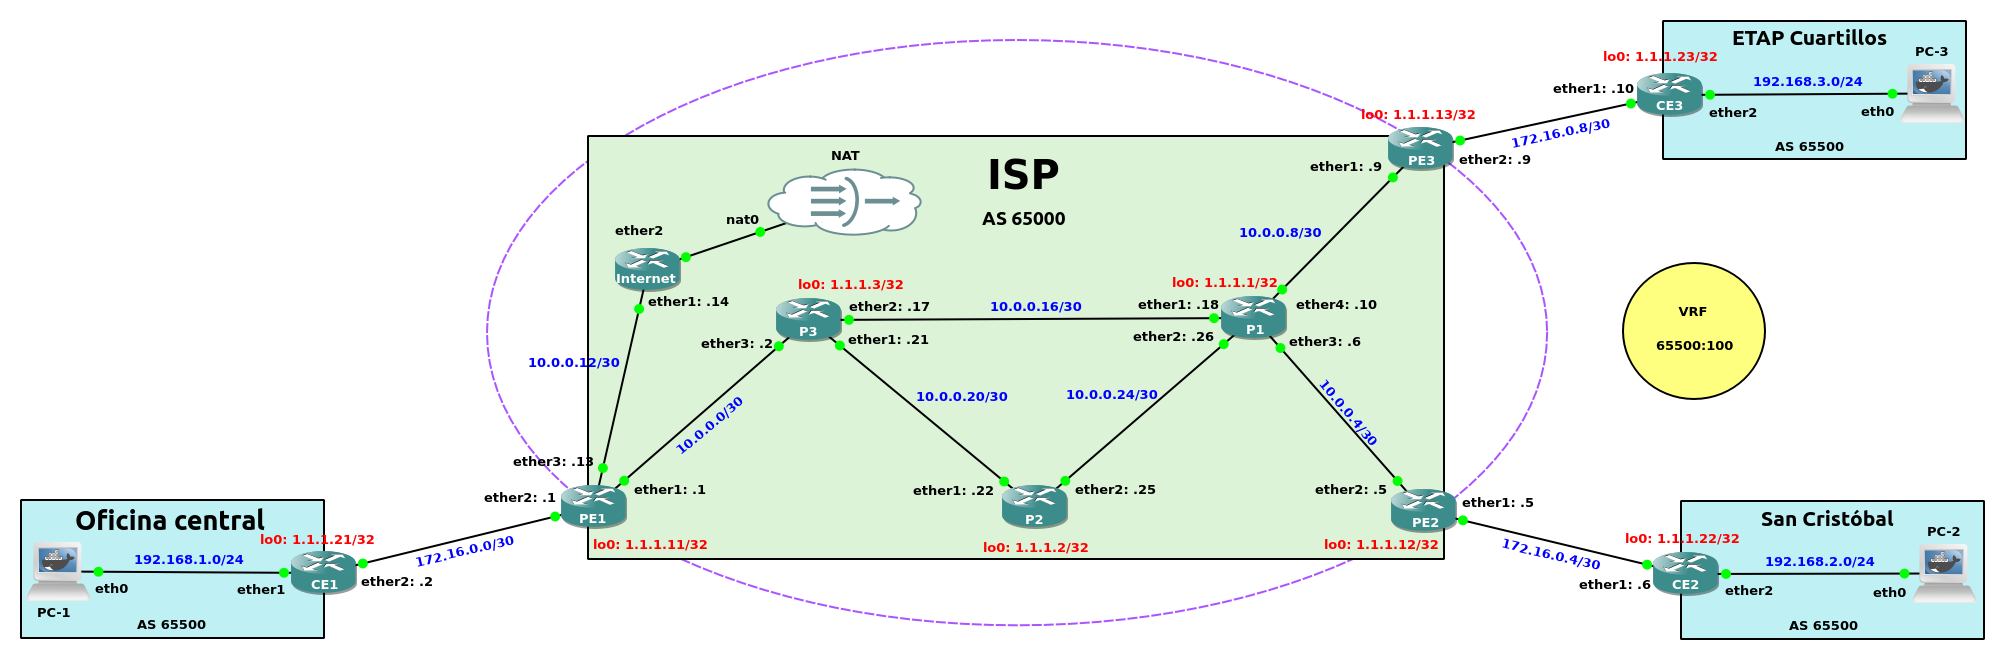
\includegraphics[width=1\textwidth]{images/red_mpls.png}
	\caption{Red MPLS configurada en GNS3}
	\label{fig:red_mpls}
\end{figure}

\newpage

\noindent
A continuación, en la Tabla~\ref{tab:esquema_direccionamiento_isp} se muestra el esquema de direccionamiento implementado en la red MPLS:
\begin{table}[H]
	\centering
	\begin{subtable}[b]{0.475\textwidth}
		\centering
		\begin{tabular}{|l|l|l|}
			\hline
			\textbf{Router} & \textbf{Interfaz} & \textbf{Dirección IP} \\ \hline
			PE1             & Lo0               & 1.1.1.11/32           \\ \cline{2-3}
			                & ether1            & 10.0.0.1/30           \\ \cline{2-3}
			                & ether2            & 172.16.0.1/30         \\ \cline{2-3}
			                & ether3            & 10.0.0.14/30          \\ \hline
			PE2             & Lo0               & 1.1.1.12/32           \\ \cline{2-3}
			                & ether1            & 172.16.0.5/30         \\ \cline{2-3}
			                & ether2            & 10.0.0.5/30           \\ \hline
			PE3             & Lo0               & 1.1.1.13/32           \\ \cline{2-3}
			                & ether1            & 10.0.0.9/30           \\ \cline{2-3}
			                & ether2            & 172.16.0.9/30         \\ \hline
			P1              & Lo0               & 1.1.1.1/32            \\ \cline{2-3}
			                & ether1            & 10.0.0.18/30          \\ \cline{2-3}
			                & ether2            & 10.0.0.26/30          \\ \cline{2-3}
			                & ether3            & 10.0.0.6/30           \\ \cline{2-3}
			                & ether4            & 10.0.0.10/30          \\ \hline
			P2              & Lo0               & 1.1.1.2/32            \\ \cline{2-3}
			                & ether1            & 10.0.0.22/30          \\ \cline{2-3}
			                & ether2            & 10.0.0.25/30          \\ \hline
		\end{tabular}
	\end{subtable}
	\hfill
	\begin{subtable}[b]{0.475\textwidth}
		\centering
		\begin{tabular}{|l|l|l|}
			\hline
			\textbf{Router} & \textbf{Interfaz} & \textbf{Dirección IP} \\ \hline
			P3              & Lo0               & 1.1.1.3/32            \\ \cline{2-3}
			                & ether1            & 10.0.0.21/30          \\ \cline{2-3}
			                & ether2            & 10.0.0.17/30          \\ \cline{2-3}
			                & ether3            & 10.0.0.2/30           \\ \hline
			CE1             & Lo0               & 1.1.1.21/32           \\ \cline{2-3}
			                & ether1            & 192.168.1.1/24        \\ \cline{2-3}
			                & ether2            & 172.16.0.2/30         \\ \hline
			CE2             & Lo0               & 1.1.1.22/32           \\ \cline{2-3}
			                & ether1            & 192.168.2.1/24        \\ \cline{2-3}
			                & ether2            & 172.16.0.6/30         \\ \hline
			CE3             & Lo0               & 1.1.1.23/32           \\ \cline{2-3}
			                & ether1            & 192.168.3.1/24        \\ \cline{2-3}
			                & ether2            & 172.16.0.10/30        \\ \hline
			Internet        & Lo0               & 1.1.1.14/32           \\ \cline{2-3}
			                & ether1            & 10.0.0.14/30          \\ \cline{2-3}
			                & ether2            & DHCP                  \\ \hline
		\end{tabular}
	\end{subtable}
	\caption{Esquema de direccionamiento para la red ISP}
	\label{tab:esquema_direccionamiento_isp}
\end{table}

Este esquema permite una gestión eficiente del tráfico entre las sedes,
garantizando la conectividad y la seguridad de los datos que circulan por la
red MPLS. Las direcciones IP asignadas a cada dispositivo son únicas dentro de
la red MPLS, lo que facilita la identificación y el enrutamiento de los
paquetes de datos.

\subsection{Configuración de interfaces loopback y asignar IPs a interfaces físicas}
En el contexto de una red MPLS, es imprescindible establecer una única sesión
LDP (Label Distribution Protocol) entre cada par de routers con el fin de
permitir el correcto intercambio de etiquetas. Para garantizar que este proceso
no se vea afectado por el estado operativo o el direccionamiento de las
interfaces físicas utilizadas para el reenvío de tráfico, se recurre
habitualmente al uso de interfaces loopback. Estas proporcionan una dirección
IP estable y siempre activa, independientemente de las condiciones de los
enlaces físicos.

\vspace{0.5cm}
En consecuencia, es necesario configurar una interfaz
loopback en cada uno de los routers que integran la infraestructura MPLS. Para
ello, se implementará una interfaz de tipo \textit{bridge} sin asociación a puertos
físicos, a la cual se asignará una dirección IP o subred previamente reservada
para las sesiones LDP dentro de la red. Esta configuración contribuye a una
mayor estabilidad y resiliencia en el establecimiento de las rutas MPLS.

\newpage

\vspace{0.5cm}
A continuación, se presenta un ejemplo de configuración de una interfaz
loopback en un router MikroTik:

\begin{lstlisting}[language=RouterOS]
[admin@MikroTik] > /system identity set name=PE1
[admin@PE2] > /interface bridge add name=lo0
[admin@PE2] > /ip address add address=1.1.1.12/32 interface=lo0
\end{lstlisting}

En cuanto a la configuración de las interfaces físicas, se han asignado
direcciones IP a las interfaces de los routers que se conectan entre sí. Por
ejemplo, en el router PE2 se ha configurado de la siguiente manera:

\begin{lstlisting}[language=RouterOS]
[admin@PE2] > /ip address add address=172.16.0.5/30 interface=ether1
[admin@PE2] > /ip address add address=10.0.0.5/30 interface=ether2
\end{lstlisting}

\subsection{OSPF como protocolo de enrutamiento}
Empezaremos aplicando el protocolo OSPF para aprender de forma dinámica las
direcciones de los routers que pertenecen a MPLS, es decir, los routers PE y P.
Por tanto, las interfaces que no pertenecen a la red MPLS no se incluirán en el
proceso de aprendizaje.

\vspace{0.5cm}  Para ello, se ha creado una instancia OSPF y se
han añadido las redes correspondientes a la misma. A continuación, se muestra
un ejemplo de configuración de OSPF en el router P1:
\begin{lstlisting}[language=RouterOS]
[admin@P1] > /routing ospf instance set redistribute-connected=as-type-1 numbers=0
[admin@P1] > /routing ospf network add area=backbone network=10.0.0.16/30 
[admin@P1] > /routing ospf network add area=backbone network=10.0.0.24/30 
[admin@P1] > /routing ospf network add area=backbone network=10.0.0.4/30 
[admin@P1] > /routing ospf network add area=backbone network=10.0.0.8/30 
\end{lstlisting}

%
% Se deberá aplicar una configuración equivalente en todos los enrutadores de la
% red MPLS, una vez hecho, por ejemplo, en P1 obtendremos la siguiente tabla de
% enrutamiento:
En la Figura~\ref{fig:routing_table} se muestra la tabla de enrutamiento del router P1, que refleja las rutas aprendidas a través del protocolo OSPF.

\begin{figure}[H]
	\centering
	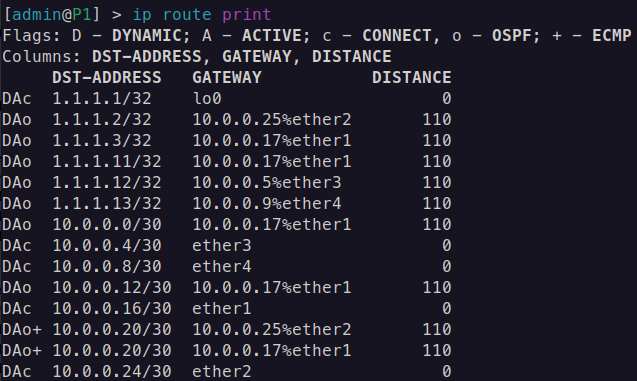
\includegraphics[width=0.8\textwidth]{images/routing_table.png}
	\caption{Tabla de enrutamiento de P1}
	\label{fig:routing_table}
\end{figure}

\subsection{Configuración de la distribución de etiquetas (LDP)}
Para asegurar la correcta distribución de las etiquetas MPLS asociadas a cada una
de las rutas activas en la red, es fundamental habilitar el Protocolo de Distribución de Etiquetas (LDP)
en todos los enrutadores que forman parte de la red MPLS. A continuación,
aplicaremos LDP sobre estos mismos routers, excluyendo las interfaces que se comunican
con routers externos a la backbone, ya que no requieren esta configuración. Esta configuración se
ha aplicado a todos los routers de la red MPLS, por ejemplo, en P1 se ha configurado de la siguiente manera:

\begin{lstlisting}[language=RouterOS]
[admin@P1] > /mpls ldp add afi=ip lsr-id=1.1.1.1 transport-addresses=1.1.1.1
[admin@P1] > /mpls ldp interface add interface=ether1
[admin@P1] > /mpls ldp interface add interface=ether2
[admin@P1] > /mpls ldp interface add interface=ether3
[admin@P1] > /mpls ldp interface add interface=ether4
\end{lstlisting}

Además, se ha configurado el rango de etiquetas dinámicas para el tráfico MPLS según la Tabla~\ref{tab:rango_etiquetas_mpls}.

\begin{table}[H]
	\centering
	\begin{tabular}{|l|l|l|}
		\hline
		\textbf{Router} & \textbf{Loopback} & \textbf{Rango de etiquetas} \\ \hline
		PE1             & 1.1.1.11          & 10000-11999                 \\ \hline
		PE2             & 1.1.1.12          & 12000-13999                 \\ \hline
		PE3             & 1.1.1.13          & 14000-15999                 \\ \hline
		P1              & 1.1.1.1           & 20000-21999                 \\ \hline
		P2              & 1.1.1.2           & 22000-23999                 \\ \hline
		P3              & 1.1.1.3           & 24000-25999                 \\ \hline
	\end{tabular}%
	\caption{Rango de etiquetas para cada router}
	\label{tab:rango_etiquetas_mpls}
\end{table}

\noindent
Para configurar el rango de etiquetas dinámicas, se ha utilizado el siguiente comando:
\begin{lstlisting}[language=RouterOS]
[admin@P1] > /mpls settings set dynamic-label-range=20000-21999
\end{lstlisting}

%
% Se repetirá el mismo proceso para los routers PE y P.

Para comprobar que la configuración es correcta, se ha realizado un \texttt{traceroute} desde el router PE1 a PE2 y
se tendrá que ver la asignación de una etiqueta.
\begin{figure}[H]
	\centering
	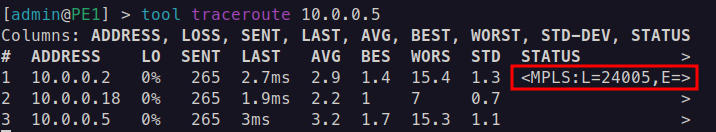
\includegraphics[width=0.8\textwidth]{images/ldp_test.png}
	\caption{Traceroute desde PE1 a PE2}
	\label{fig:traceroute}
\end{figure}

\subsection{Multi-Protocolo BGP (MP-BGP)}
El Multi-Protocolo BGP (MP-BGP) es una extensión del protocolo BGP (Border Gateway Protocol) que permite propagar direcciones y los atributos que la acompañan a través de múltiples protocolos de red. En este contexto, los Sistemas Autónomos (AS) representan agrupaciones de redes bajo una misma política de enrutamiento, lo que facilita la gestión y el intercambio de rutas entre diferentes dominios administrativos. Por tanto, para establecer la conectividad entre los routers PE de la red MPLS, se creará una sesión BGP entre ellos. Para ello, primero se actualizará la plantilla \texttt{default} de BGP en los routers, acorde al sistema autónomo (65000 en este caso) y al conjunto de direcciones que enrutará cada router PE.

\vspace{0.5cm}
\noindent
A continuación, se muestra un ejemplo de configuración de BGP en el router PE2:
\begin{lstlisting}[language=RouterOS]
[admin@PE2] > /routing bgp template set default address-families=ip,vpnv4 as=65000 router-id=1.1.1.12
\end{lstlisting}

Ahora, se crearán las conexiones BGP entre los otros routers PE de la red MPLS. Unicamente hay que configurar la dirección local, la dirección remota, el AS remoto, el role local de BGP (ibgp en este caso al ser routers de la misma AS) y habilitar la escucha como la conexión.
\begin{lstlisting}[language=RouterOS]
[admin@PE2] > /routing bgp connection add name=toPE1 template=default local.address=1.1.1.12 local.role=ibgp remote.address=1.1.1.11 remote.as=65000 connect=yes listen=yes
[admin@PE2] > /routing bgp connection add name=toPE3 template=default local.address=1.1.1.12 local.role=ibgp remote.address=1.1.1.13 remote.as=65000 connect=yes listen=yes
[admin@PE2] > /routing bgp connection add name=toPE4 template=default local.address=1.1.1.12 local.role=ibgp remote.address=1.1.1.14 remote.as=65000 connect=yes listen=yes
\end{lstlisting}

Una vez hecho, se podrá comprobar que se ha establecido la sesión BGP ejecutando el comando \lstinline[language=RouterOS]|/routing bgp session print| en los routers PE:

\begin{figure}[H]
	\centering
	\begin{subfigure}[b]{0.475\textwidth}
		\centering
		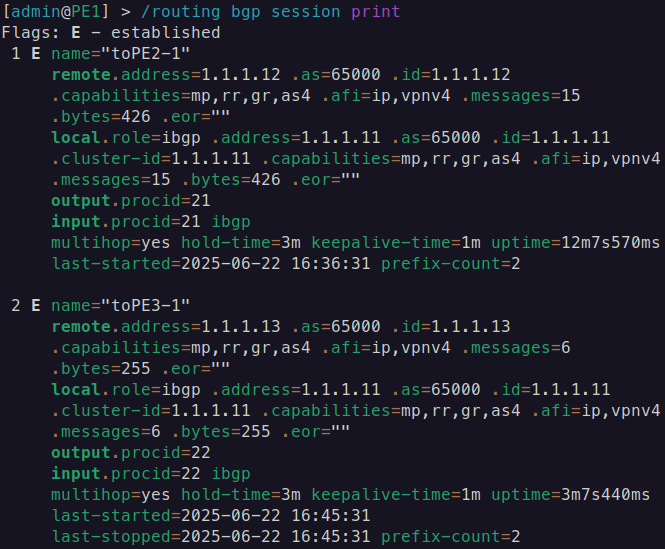
\includegraphics[width=\textwidth]{images/PE1_bgp_print.png}
		\caption{Sesiones BGP establecidas en PE1}
		\label{fig:PE1_bgp_print}
	\end{subfigure}
	\hfill
	\begin{subfigure}[b]{0.482\textwidth}
		\centering
		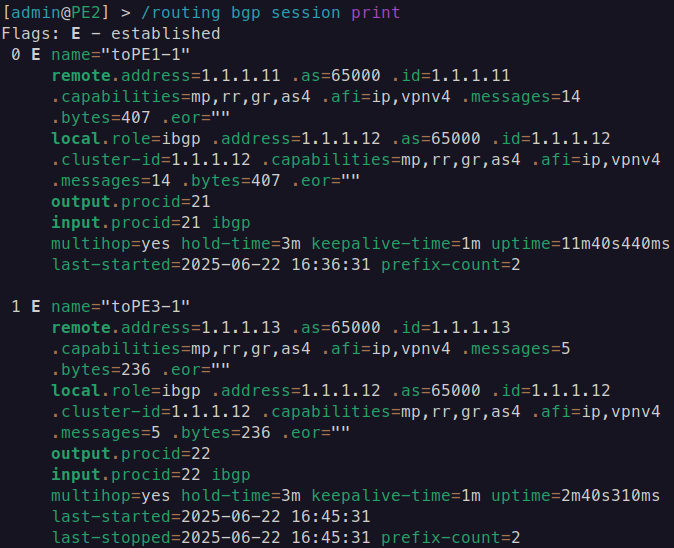
\includegraphics[width=\textwidth]{images/PE2_bgp_print.png}
		\caption{Sesiones BGP establecidas en PE2}
		\label{fig:PE2_bgp_print}
	\end{subfigure}
	\caption{Sesiones BGP establecidas en PE1 y PE2}
	\label{fig:PE1_PE2_PE3_bgp_print}
\end{figure}

\subsection{Configuración de VRF y VPN}
Virtual Routing and Forwarding (VRF) es una tecnología que permite que múltiples
instancias de una tabla de enrutamiento coexistan en el mismo router. Las sedes se
situarán en una tabla VRF configurada con un RD (Route Distinguisher) y un RT (Route Target)
de importación y exportación. El RD es un identificador de rutas VPN que se antepone a la dirección
de red para formar un prefijo único (ASN:número de ruta). El RT es el valor numérico definido por
cada PE que está asociado a las rutas que exporta a los puertos BGP. Existen dos tipos de RT:

\begin{itemize}
	\item \textbf{RT de exportación:} Identifican los sitios remotos a los que se exportan las rutas.
	\item \textbf{RT de importación:} Utilizados por los routers PE para importar las rutas en sus tablas VRF.
\end{itemize}

Para la configuración, antes se crearán las VRFs unicamente en los routers PE que servirán para consultar el direccionamiento de las sedes que están conectadas a la red MPLS. Se creará una tabla VRF por router PE de la siguiente manera:
\begin{lstlisting}[language=RouterOS]
[admin@PE2] > /ip vrf add name=CE2 interfaces=ether1 
\end{lstlisting}

Ahora, se configurará la VPN a través de BGP en los routers PE. Se definirá el \texttt{Router Distinguishers (RD)}, el cual identifica la ruta VPN y es representado como ASN:número de ruta.

\vspace{0.5cm}
También se definirán los \texttt{Route Target (RT)} de exportación y de importación, que indicarán qué rutas se distribuirán al peer PE según la VPN que identifique. En este caso, se ha definido el mismo valor para RD y RT.

\vspace{0.5cm}
Finalmente, se especificará la política de asignación de etiquetas, la tabla VRF que se empleará y el tipo de rutas que se compartirán desde la VRF hacia VPNv4. Además de las rutas estáticas (static) y conectadas (connected), se activará BGP, dado que este será el protocolo utilizado entre los routers PE y CE en su variante External BGP (eBGP).

\begin{lstlisting}[language=RouterOS]
[admin@PE2] > /routing bgp vpn add route-distinguisher=65000:100 import.route-targets=65000:100 vrf=CE2 label-allocation-policy=per-vrf export.route-targets=65000:100 .redistribute=connected,static,bgp
\end{lstlisting}

\subsection{Comunicación entre routers PE y CE}
Para garantizar la conectividad entre los routers PE y CE, implementaremos el protocolo eBGP, asignando un número de sistema autónomo (AS) distinto al de la red troncal MPLS, específicamente el AS 65500.

\subsubsection*{Configuración de los routers PE}
En los routers PE, se van a crear nuevas conexiones BGP con los routers CE. Se va a indicar la dirección local, el AS local, el role local, el AS remoto, la dirección remota, y a habilitar la conexión y la escucha. Además, hay que indicar el ID del router que será la interfaz loopback, el \texttt{VRF} que se usará y la tabla de routing asociada al \texttt{VRF}. Por último, para asegurar que todas las rutas puedan ser anunciadas por la red MPLS, es necesario configurar \texttt{output.default-originate=always}. Esta acción genera una ruta por defecto en el router CE, la cual se aprende mediante eBGP y es crucial para la comunicación de direcciones privadas a través de MPLS.

\begin{lstlisting}[language=RouterOS]
[admin@PE2] > /routing bgp connection add name=toCE2 router-id=1.1.1.12 as=65000 local.address=172.16.0.5 .role=ebgp remote.address=172.16.0.6 .as=65500 routing-table=CE2 vrf=CE2 connect=yes listen=yes output.default-originate=always
\end{lstlisting}

\subsubsection*{Configuración de los routers CE}
Para los routers CE, hay una lista de direcciones que se van a exportar a través de BGP. En esta lista de direcciones se asignarán a la conexión BGP para permitir que los paquetes recibidos en el CE puedan ser enviados a través de la red MPLS.
\begin{lstlisting}[language=RouterOS]
[admin@CE2] > /ip firewall address-list add address=192.168.2.0/24 list=BGP_OUT
\end{lstlisting}

Ahora con la lista direcciones creada, se puede configurar la conexión BGP entre el router CE y el router PE. Se indicará el ID del router, AS, dirección local, role local, dirección remota, AS remoto y la lista de direcciones que se van a exportar. También se activará la conexión y la escucha.
\begin{lstlisting}[language=RouterOS]
[admin@CE2] > /routing bgp connection add name=toPE2 as=65500 router-id=1.1.1.22 local.address=172.16.0.6 .role=ebgp remote.address=172.16.0.5 remote.as=65000 output.network=BGP_OUT connect=yes listen=yes
\end{lstlisting}

Con las conexiones BGP configuradas, se puede comprobar que se ha establecido la sesión BGP ejecutando el comando \lstinline[language=RouterOS]|/routing bgp session print| en los routers CE:

\begin{figure}[H]
	\centering
	\begin{subfigure}[b]{0.48\textwidth}
		\centering
		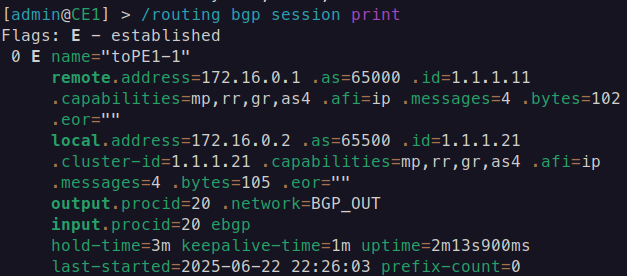
\includegraphics[width=\textwidth]{images/CE1_bgp_print.png}
		\caption{Sesiones BGP establecidas en CE1}
		\label{fig:CE1_bgp_print}
	\end{subfigure}
	\hfill
	\begin{subfigure}[b]{0.48\textwidth}
		\centering
		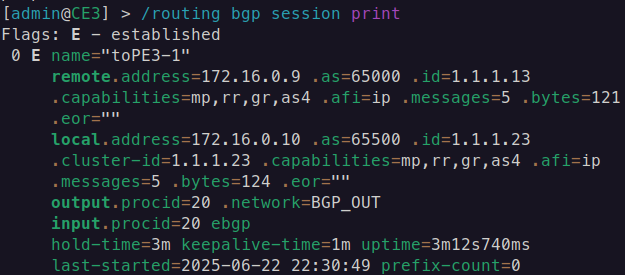
\includegraphics[width=\textwidth]{images/CE3_bgp_print.png}
		\caption{Sesiones BGP establecidas en CE3}
		\label{fig:CE3_bgp_print}
	\end{subfigure}
	\caption{Sesiones BGP establecidas en los routers CE}
	\label{fig:bgp_sessions}
\end{figure}

\begin{tcolorbox}[colback=gray!10!white, colframe=gray!70!black, title=NOTA:, size=title]
	\textit{Todas las configuraciones mostradas en los ejemplos anteriores se aplicarán de forma análoga en el resto de los routers, adaptando únicamente las direcciones IP, nombres de interfaces y parámetros específicos según corresponda a cada dispositivo.}
\end{tcolorbox}

\subsection{Acceso a Internet}
% PE1:
% /routing bgp template set default address-families=ip,vpnv4 as=65000 router-id=1.1.1.11
% /routing bgp connection
% add connect=yes disabled=no listen=yes local.address=1.1.1.11 .role=ibgp \
%     name=toPE2 remote.address=1.1.1.12 .as=65000 templates=default
% /routing bgp connection
% add connect=yes disabled=no listen=yes local.address=1.1.1.11 .role=ibgp \
%     name=toPE3 remote.address=1.1.1.13 .as=65000 templates=default
% /routing bgp connection
% add connect=yes disabled=no listen=yes local.address=1.1.1.11 .role=ibgp \
%     name=toPE4 remote.address=1.1.1.14 .as=65000 templates=default

% /ip vrf add name=CE1 interfaces=ether2 

% /routing bgp vpn
% add export.redistribute=connected,static,bgp .route-targets=65000:100 \
%     import.route-targets=65000:100 label-allocation-policy=per-vrf name=\
%     bgp-mpls-vpn-1 route-distinguisher=65000:100 vrf=CE1

% /routing bgp connection
% add as=65000 connect=yes disabled=yes listen=yes local.address=172.16.0.1 \
%     .role=ebgp name=toCE1 output.default-originate=always remote.address=\
%     172.16.0.2 .as=65500 router-id=1.1.1.11 routing-table=CE1 vrf=CE1

% /routing bgp connection add as=65000 connect=yes disabled=yes listen=yes local.address=172.16.0.1 .role=ebgp name=toCE1 output.default-originate=always remote.address=172.16.0.2 .as=65500 router-id=1.1.1.11 routing-table=CE1 vrf=CE1

% /ip firewall mangle
% add action=mark-routing chain=prerouting dst-address=!192.168.0.0/16 \
%     in-interface=ether2 new-routing-mark=main passthrough=yes
% /ip route add gateway=172.16.0.2@CE1 routing-table=CE1
% /ip route add gateway=10.0.0.14
% /ip route add dst-address=172.16.0.0/30 gateway=CE1@CE1 routing-table=main

% % CE1:
% /ip firewall address-list add address=192.168.1.0/24 list=BGP_OUT
% /ip firewall nat add action=masquerade chain=srcnat dst-address=!192.168.0.0/16 out-interface=ether2

% /ip route add gateway=172.16.0.1

% /routing bgp connection
% add as=65500 connect=yes listen=yes local.address=172.16.0.2 .role=ebgp name=\
%     toPE1 output.network=BGP_OUT remote.address=172.16.0.1 .as=65000 router-id=\
%     1.1.1.21


Para proporcionar acceso a Internet se ha centralizado en el router CE1 que este actuará como gateway, es decir todo el tráfico que quiera salir a Internet pasará por este router y luego volverá al router PE1 y de ahi a otro router que se conecta a Internet. Para ello, se ha configurado el router CE1 para que realice NAT (Network Address Translation) y permita que los dispositivos una red local accedan a Internet. Además, se ha quitado la conexión BGP entre el router PE1 y CE1, añadiendo una ruta estática en el router PE1 hacia CE1 dentro de la VRF CE1. La configuración de la conexión BGP entre el router PE1 y CE1 se ha realizado de la siguiente manera:
\begin{lstlisting}[language=RouterOS]
[admin@PE1] > /routing bgp connection
add as=65000 connect=yes disabled=yes listen=yes local.address=172.16.0.1 .role=ebgp name=toCE1 output.default-originate=always remote.address=172.16.0.2 .as=65500 router-id=1.1.1.11 routing-table=CE1 vrf=CE1
\end{lstlisting}

Para que el router CE1 pueda realizar NAT, se ha configurado una regla de NAT que permite que el tráfico que sale por la interfaz \texttt{ether2} (que es la interfaz conectada a Internet) sea traducido. La configuración de la regla de NAT se ha realizado de la siguiente manera:
\begin{lstlisting}[language=RouterOS]
[admin@CE1] > /ip firewall nat add action=masquerade chain=srcnat dst-address=!192.168.0.0/16 out-interface=ether2
\end{lstlisting}

Además, se ha configurado una ruta estática en el router CE1 para que el tráfico que sale a Internet pase por la interfaz \texttt{ether2}. La configuración de la ruta estática se ha realizado de la siguiente manera:
\begin{lstlisting}[language=RouterOS]
[admin@CE1] > /ip route add gateway=172.16.0.1
\end{lstlisting}

Para que el router CE1 pueda enviar tráfico a la red local, se ha configurado una ruta estática en el router PE1 hacia CE1 dentro de la VRF CE1. La configuración de la ruta estática se ha realizado de la siguiente manera:
\begin{lstlisting}[language=RouterOS]
[admin@PE1] > /ip route add dst-address=172.16.0.0/30 gateway=CE1@CE1 routing-table=main
[admin@PE1] > /ip route add gateway=172.16.0.2@CE1 routing-table=CE1
\end{lstlisting}

Por otro lado, para que el tráfico que sale por la interfaz \texttt{ether2} del router PE1 se enrute correctamente, se ha configurado una regla de mangle que marca el tráfico que no es de la red local (192.168.0.0/16) y lo enruta a través de la tabla de enrutamiento principal. La configuración de la regla de mangle se ha realizado de la siguiente manera:
\begin{lstlisting}[language=RouterOS]
[admin@PE1] > /ip firewall mangle add action=mark-routing chain=prerouting dst-address=!192.168.0.0/16 in-interface=ether2 new-routing-mark=main passthrough=yes
\end{lstlisting}

\subsection{Comprobación de la configuración}
Para comprobar que la configuración es correcta se hará un \texttt{ping} entre los PCs, por ejemplo, desde el PC1 a la IP 192.168.2.100. Pero antes hay que configurar la IP estática. Para ello, se edita el archivo \texttt{/etc/network/interfaces} y añadiendo la siguiente configuración:
\begin{lstlisting}[language=bash]
auto eth0
iface eth0 inet static
	address 192.168.X.100
	netmask 255.255.255.0
	gateway 192.168.X.1
\end{lstlisting}

\begin{tcolorbox}[colback=gray!10!white, colframe=gray!70!black, title=NOTA:, size=title]
	La X será según en que sede esté el PC. Por ejemplo, si el PC está en la Oficina Central, la X será 1.
\end{tcolorbox}

Una vez configurada la IP estática, se puede comprobar que la configuración es correcta como se ve en la Figura~\ref{fig:ping_test}.
\begin{figure}[H]
	\centering
	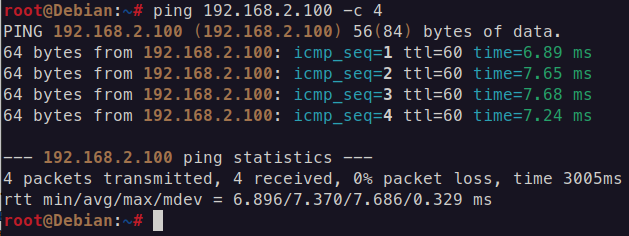
\includegraphics[width=0.75\textwidth]{images/ping_test.png}
	\caption{Comprobación de la configuración}
	\label{fig:ping_test}
\end{figure}

\section{Simulación de la Oficina Central}
La oficina central se ha configurado con un prefijo global de 2001:db8:1234:0100::/56 y
se han creado tres VLANs para segmentar el tráfico de datos, voz y DMZ. La VLAN
10 se ha asignado para el tráfico de datos, la VLAN 20 para el tráfico de voz y
la VLAN 30 para la DMZ. Por otro lado, esta sede contará con dos routers CE
(Customer Edge) configurados en alta disponibilidad mediante el protocolo VRRP
(Virtual Router Redundancy Protocol) \cite{wikipedia_vrrp}. Además, se ha configurado
un servidor DHCP para asignar direcciones IP dinámicamente a los dispositivos de la red
local y dos servidores DNS para resolver nombres de dominio y direcciones IP. La topología de switching
implementa el protocolo RSTP (Rapid Spanning Tree Protocol) \cite{wikipedia_rstp} para garantizar
redundancia en los enlaces y prevenir bucles de red, asegurando una convergencia
rápida ante fallos.
\begin{figure}[H]
	\centering
	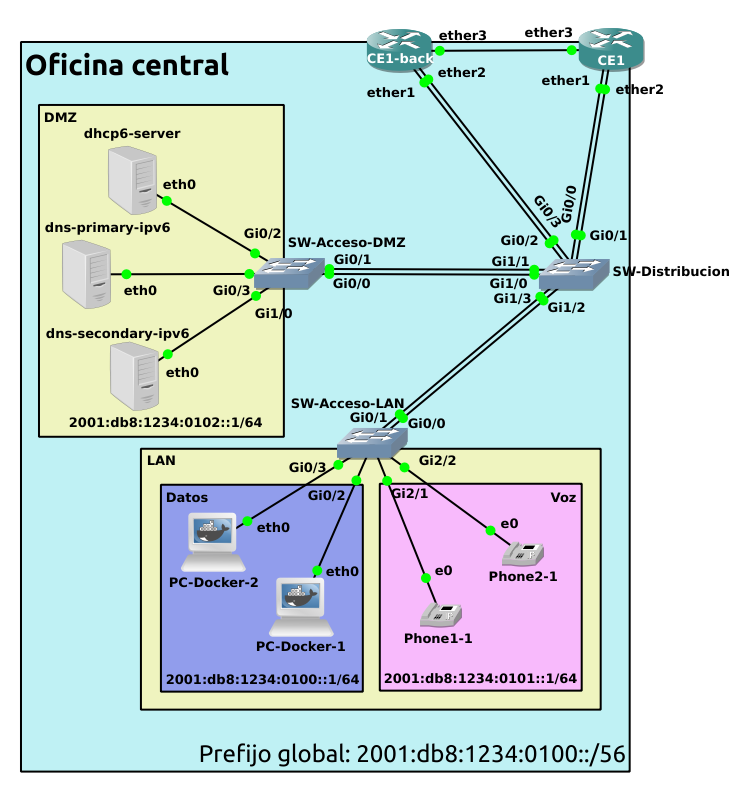
\includegraphics[width=0.8\textwidth]{images/central_office.png}
	\caption{Esquema de la oficina central}
	\label{fig:central_office}
\end{figure}

\subsection{Configuración de los routers}
Para la red local se han utilizado dos routers MikroTik CE1 \ref{Apendice2:configuracion_ce1} y CE1\_backup \ref{Apendice2:configuracion_ce1_backup} configurados con alta disponibilidad mediante VRRP y conectados a través de un enlace de sincronización dedicado. Ambos dispositivos emplean un bonding LACP (802.3ad) sobre dos interfaces físicas para mejorar la redundancia y el ancho de banda. Sobre este bonding se han definido tres VLANs: datos, voz
y DMZ, a cada una de las cuáles se le asigna una dirección IPv6. En cada VLAN se implementa VRRP, configurando CE1 como maestro (prioridad 150) y CE1\_backup como respaldo (prioridad 100), y se asignan direcciones virtuales que actúan como gateway para los dispositivos de la red. Además, se configura un relay DHCPv6 en las VLANs de datos y voz, se anuncian los servidores DNS mediante Neighbor Discovery \cite{wikipedia_nd} y se aplica un firewall básico para IPv6.

\vspace{0.5cm}
Para comprobar el funcionamiento de la configuración VRRP, se a ha ejecutado en el router CE1 el comando \lstinline[language=RouterOS]|/interface vrrp print| y se ha obtenido lo que se muestra en la Figura~\ref{fig:vrrp_output_1}.

\begin{figure}[H]
	\centering
	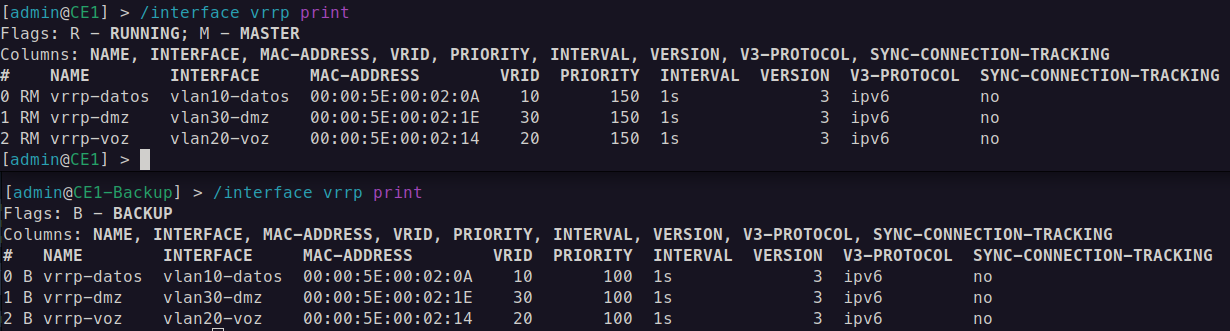
\includegraphics[width=1\textwidth]{images/vrrp_output_1.png}
	\caption{Estado de los VRRP en el router CE1}
	\label{fig:vrrp_output_1}
\end{figure}

Al ejecutar el comando, en el CE1, se puede observar que están las letras \texttt{R} y \texttt{M} que significa que están en \textit{RUNNING} y \textit{MASTER} respectivamente, confirmando que es el router maestro de VRRP. Además, se puede ver que el \texttt{Priority} es 150, es decir, que tiene más prioridad que el router CE1\_Backup que tiene el
\texttt{Priority} en 100. Otra prueba que se hizo es apagar temporalmente la interfaz VLAN 10 del router CE1 y se puede ver que el router CE1\_Backup se convierte en maestro en esta interfaz, siendo anterior el maestro. En la Figura~\ref{fig:vrrp_output_2} se puede ver el estado de los VRRP en el router CE1\_Backup.
\begin{figure}[H]
	\centering
	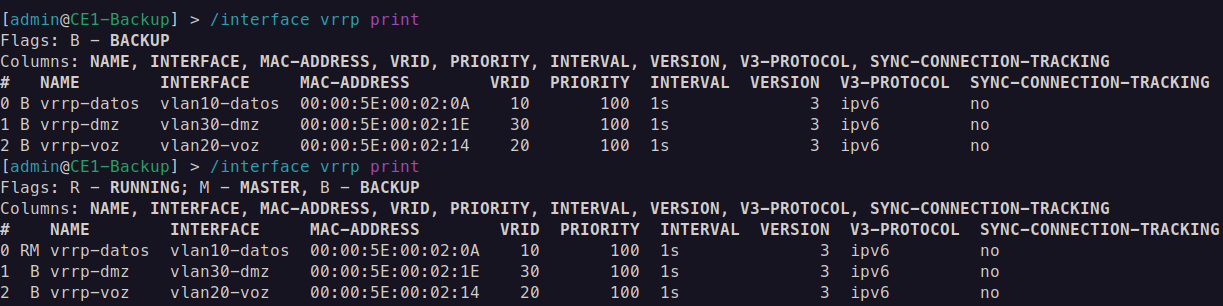
\includegraphics[width=1\textwidth]{images/vrrp_output_2.png}
	\caption{Estado de los VRRP en el router CE1\_Backup}
	\label{fig:vrrp_output_2}
\end{figure}

Otra comprobación, como se muestra en la Figura~\ref{fig:test_DHCP6_pc}, es la correcta asignación de direcciones IPv6 y conectividad con la interfaz VRRP de cada VLAN. En la izquierda
un telefono en la VLAN 20 y en la derecha un PC en la VLAN 10.

\begin{figure}[H]
	\centering
	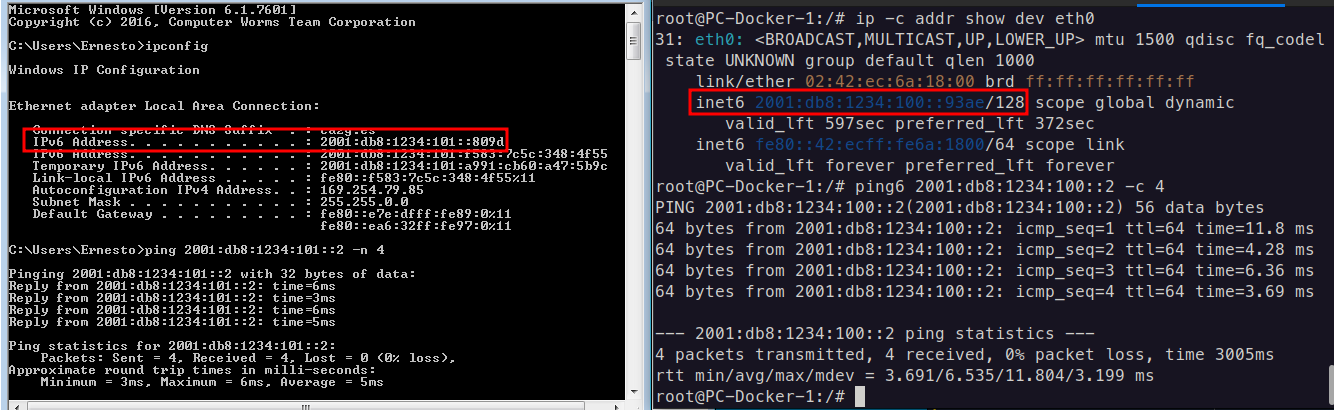
\includegraphics[width=1\textwidth]{images/test_DHCP6_ping.png}
	\caption{Asignación y conectividad IPv6}
	\label{fig:test_DHCP6_pc}
\end{figure}

Además, si desde un host se pide otra dirección IPv6, se puede ver que se obtiene una dirección ofrecida por el relay DHCPv6. En la Figura~\ref{fig:dhclient_ok} se puede ver que un host de la VLAN 10 obtiene la dirección 2001:db8:1234:100::93ae.

\begin{figure}[H]
	\centering
	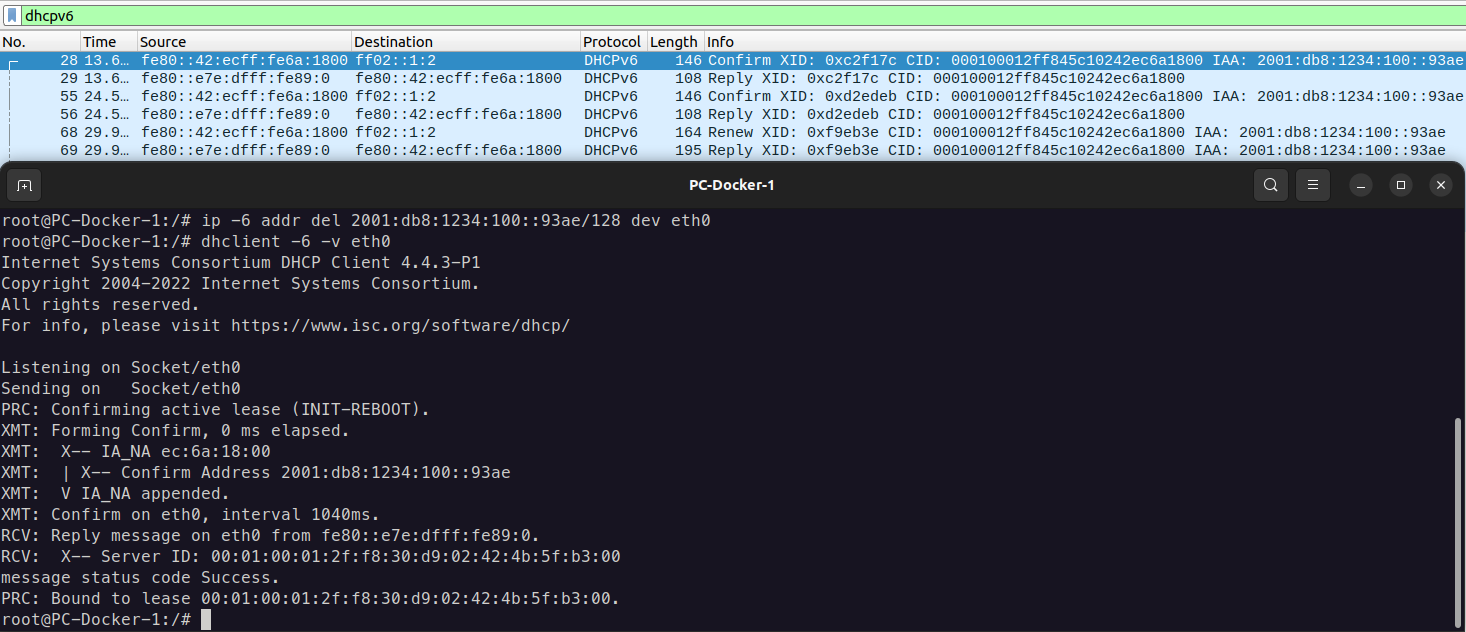
\includegraphics[width=0.95\textwidth]{images/dhclient_ok.png}
	\caption{Obtención de una dirección IPv6}
	\label{fig:dhclient_ok}
\end{figure}

% \begin{itemize}
%     \item Comprobación de la correcta asignación de direcciones IPv6 y conectividad entre hosts de cada VLAN.
%     \item Verificación del funcionamiento del failover de VRRP: ante la caída del router maestro (CE1), el router de respaldo (CE1\_backup) asume el rol de maestro sin pérdida de conectividad.
%     \item Prueba del relay DHCPv6: los hosts de las VLANs de datos y voz obtienen direcciones IPv6 dinámicas correctamente.
%     \item Comprobación de la recepción de los servidores DNS mediante Neighbor Discovery (RA).
%     \item Prueba de la comunicación entre ambos routers a través del enlace de sincronización dedicado.
% \end{itemize}

\subsection{Configuración de los switches}
En la simulación se han utilizado tres switches: uno de distribución \ref{Apendice2:configuracion_switch_distribucion_central} y dos de acceso. El switch de distribución se encarga de conectar los switches de acceso, uno a la red local \ref{Apendice2:configuracion_switch_acceso_lan_central} y otro a la DMZ \ref{Apendice2:configuracion_switch_acceso_dmz_central}. Los switches de acceso conectan los dispositivos finales a la red.

\vspace{0.5cm}
Se han configurado las VLANs en los switches para segmentar el tráfico de datos, voz y DMZ. Además, se ha implementado el protocolo Rapid Spanning Tree Protocol (RSTP), que permite una convergencia más rápida ante fallos de enlace en comparación con el STP tradicional.

\vspace{0.5cm}
Por otra parte, para aprovechar los enlaces redundantes entre los switches y aumentar el rendimiento de la red, se ha implementado EtherChannel utilizando el protocolo LACP (Link Aggregation Control Protocol). Esto permite agrupar múltiples enlaces físicos en un único enlace lógico, lo cual proporciona redundancia y balanceo de carga sin que los puertos se bloqueen por RSTP.

\vspace{0.5cm}
Para verificar el funcionamiento de RSTP, se ha utilizado el comando \lstinline[language=CiscoIOS]|show spanning-tree| en los switches, que muestra el estado de las VLANs y sus interfaces asociadas. Como ejemplo, desde el switch de acceso a la LAN, al ejecutar el comando
\lstinline[language=CiscoIOS]|show spanning-tree vlan 10|, se obtiene lo que se muestra en la Figura~\ref{fig:spanning_tree_vlan10}, donde se puede ver que el protocolo RSTP está habilitado y funcionando adecuadamente, y que el Root Bridge de la VLAN 10 es el switch de distribución. También, el enlace hacia el Root Bridge se establece a través
de la interfaz Port-channel4, correspondiente a un EtherChannel configurado con LACP, que se encuentra en estado Root Forwarding. Esto indica que el enlace lógico está activo y es utilizado como camino principal hacia el Root Bridge, sin necesidad de bloquear enlaces físicos. Luego, los demás puertos del switch aparecen en estado Designated Forwarding, lo que demuestra que están activos y conectan con los dispositivos finales. El hecho de que no existan puertos en estado de bloqueo confirma que EtherChannel está funcionando, evitando bucles sin que RSTP tenga que bloquear enlaces individuales.

\begin{figure}[htb]
	\centering
	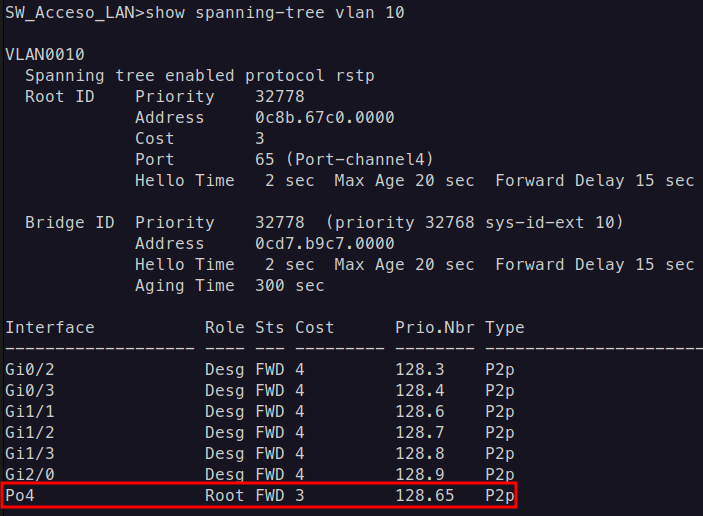
\includegraphics[width=0.7\textwidth]{images/testSTP_SWLAN2SWDistribucion_Central.png}
	\caption{Estado del protocolo Spanning Tree}
	\label{fig:spanning_tree_vlan10}
\end{figure}

\subsection{Configuración del servidor DHCP}
Para el servidor DHCP, se ha utilizado \texttt{isc-dhcp-server} sobre un contenedor Docker basado en Ubuntu 20.04, con una configuración automatizada mediante un Dockerfile \ref{Apendice2:dockerfile_dhcp}. El servidor se ha configurado con una IP estática 2001:db8:1234:0102::132/64 y se han definido rangos de direcciones IP para cada segmento de red, asegurando que los dispositivos conectados reciban direcciones válidas según el segmento al que pertenezcan. El archivo de configuración principal se encuentra en \texttt{/etc/dhcp/dhcpd6.conf} \ref{Apendice2:dhcpd6.conf}, donde se especifican los tiempos de concesión, las opciones de dominio y servidores DNS, así como las subredes correspondientes. Para las VLANs se han definido los siguientes rangos de direcciones IPv6:
\begin{itemize}
	\item \textbf{Red de datos:} rango \texttt{2001:db8:1234:0100::2} a \texttt{2001:db8:1234:0100::ffff}.
	\item \textbf{Red de voz:} rango \texttt{2001:db8:1234:0101::2} a \texttt{2001:db8:1234:0101::ffff}.
	\item \textbf{DMZ:} no se ha configurado DHCP, ya que los dispositivos en esta red tienen direcciones estáticas.
\end{itemize}

Por otro lado, el archivo \texttt{isc-dhcp-server} se especifica la interfaz de red que utilizará el servidor DHCP
para escuchar las solicitudes de los clientes. En este caso, se ha configurado para que escuche en la interfaz \texttt{eth0}, por lo que se ha añadido la siguiente línea al archivo de configuración: \lstinline[language=bash]|INTERFACESv6="eth0"|

\subsection{Configuración de los servidores DNS}
Para la infraestructura DNS, se han implementado dos servidores DNS utilizando \texttt{bind9} en contenedores Docker, uno como servidor primario y otro como secundario, ambos basados en Ubuntu 20.04. La configuración de los servidores DNS se ha realizado de manera que se garantice la alta disponibilidad y la resolución de nombres de dominio para la red local.

\subsubsection*{Servidor DNS primario}
El servidor DNS primario se va a configurar con la IP 2001:db8:1234:0102::133/64.
El archivo de configuración principal de \texttt{bind9} se encuentra en \texttt{/etc/bind/named.conf.options} \ref{Apendice2:named.conf.options}. Aqui se especifica que el servidor escuchará únicamente en IPv6, se define el rango de direcciones IP autorizadas para consultas y transferencias, se configuran los servidores de reenvío para consultas externas, y se habilita la recursión para las redes autorizadas. Además, se habilita la validación DNSSEC para mejorar la seguridad de las respuestas DNS.

\vspace{0.5cm}
Por otro lado, en \texttt{/etc/bind/named.conf.local} \ref{Apendice2:named.conf.local} se configuran las zonas DNS. Este archivo define dos zonas: una zona directa para el dominio \texttt{cazg.es} y una zona inversa para la red de servicios \texttt{2001:db8:1234:0102::/64}. La zona directa permite resolver nombres de dominio a direcciones IP, mientras que la zona inversa permite resolver direcciones IP a nombres de dominio. En ambas zonas, se especifica el
servidor de nombres primario (ns1.cazg.es) y se permite la transferencia de zona al servidor secundario (ns2.cazg.es) para garantizar la sincronización de la información entre ambos servidores.

\vspace{0.5cm}
Por otro lado, el archivo de zona directa \texttt{/etc/bind/zones/db.cazg.es} \ref{Apendice2:db.cazg.es} contiene la configuración de los registros DNS para el dominio \texttt{cazg.es}. Se define el registro SOA (Start of Authority) que indica el servidor de nombres principal para el dominio, así como los registros NS (Name Server) que especifican los servidores de nombres autoritativos para el dominio. También se incluyen registros AAAA para los servidores DNS y el servidor DHCP, que permiten la resolución de nombres a direcciones IPv6.

\vspace{0.5cm}
El archivo de zona inversa \texttt{/etc/bind/zones/db.2001.db8.1234.0102} \ref{Apendice2:db.2001.db8.1234.0102} se define el registro SOA que indica el servidor de nombres principal para la zona inversa, así como los registros NS que especifican los servidores de nombres autoritativos para la zona. También se incluyen registros PTR (Pointer) que permiten la resolución inversa de direcciones IPv6 a nombres de dominio, facilitando la identificación de los servidores DNS y el servidor DHCP en la red de servicios.

\subsubsection*{Servidor DNS secundario}
El servidor DNS secundario va a tener la IP estática 2001:db8:1234:0102::134/64 y la configuración es similar a la del servidor primario, pero se debe especificar que es un servidor esclavo y se debe indicar la IP del servidor primario para las transferencias de zona. El archivo de configuración principal \texttt{/etc/bind/named.conf.options} \ref{Apendice2:named.conf.options_dns2} se especifica que el servidor escuchará únicamente en IPv6, se define el rango de direcciones IP autorizadas para consultas, se configuran los servidores de reenvío para consultas externas, y se habilita la recursión para las redes autorizadas. Además, se habilita la validación DNSSEC para mejorar la seguridad de las respuestas DNS.

\vspace{0.5cm}
Las zonas DNS se definen en el archivo \texttt{/etc/bind/named.conf.local} \ref{Apendice2:named.conf.local_dns2}. En este archivo, se configuró como un esclavo para las zonas directas e inversas, y se especifica la IP del servidor primario para las transferencias de zona. El archivo de zona directa \texttt{db.cazg.es} y el archivo de zona inversa \texttt{db.2001.db8.1234.0102} serán idénticos a los del servidor primario, ya que el servidor secundario replicará la información de las zonas desde el primario.

\vspace{0.3cm}
\begin{tcolorbox}[colback=gray!10!white, colframe=gray!70!black, title=NOTA:, size=title]
	\textit{Para que los servidores DNS y DHCP puedan comunicarse con los dispositivos de la red en GNS3 se ha creado una red personalizada de Docker llamada \texttt{services\_net} que permite la comunicación entre los contenedores y los dispositivos de la red. Esta red se ha configurado con el controlador \texttt{bridge} y se ha habilitado IPv6 para permitir la comunicación con las direcciones IPv6 de la red.}
\end{tcolorbox}

\subsection{Configuración de los hosts}
Para los dispositivos finales de acceso a la red se ha creado un contenedor Docker personalizado basado en Debian Bookworm \cite{debian_bookworm} que actúa como PC de
prueba para realizar comprobaciones de conectividad y funcionalidad de red en el entorno de simulación. Esta decisión se tomó debido a las limitaciones
de recursos computacionales del equipo de desarrollo, ya que los contenedores Docker consumen significativamente menos recursos hardware comparado
con máquinas virtuales completas.

\vspace{0.5cm}
El contenedor se ha configurado con privilegios elevados para permitir la manipulación de interfaces de red y se ha habilitado explícitamente IPv6 mediante la configuración de parámetros del kernel. El Dockerfile \ref{Apendice2:dockerfile_network_test} incluye múltiples herramientas de red esenciales para realizar pruebas exhaustivas de conectividad y diagnóstico.

\vspace{0.5cm}
El script de entrada (\texttt{entrypoint.sh}) \ref{Apendice2:entrypoint_network_test} configura automáticamente los servidores DNS al arranque del contenedor, estableciendo los servidores DNS primario y secundario de la red de servicios.

\vspace{0.5cm}
Esta configuración permite que el contenedor pueda resolver nombres de dominio desde el inicio, facilitando las pruebas de conectividad y la verificación del funcionamiento de los servicios DNS. El contenedor se mantiene activo ejecutando bash, permitiendo realizar pruebas interactivas y comandos de diagnóstico de red. Se puede desplegar fácilmente utilizando Docker Compose \ref{Apendice2:docker_compose_network_test}, lo que simplifica su gestión y permite su integración con el entorno de simulación de GNS3, proporcionando una herramienta versátil para realizar pruebas exhaustivas de la funcionalidad de red, incluyendo la verificación de conectividad IPv6, resolución DNS, asignación DHCP y análisis de tráfico de red.

\section{Simulación entre sedes remotas y red ISP}
\label{sec:simulacion_completa}
Para este caso, se ha intentado realizar una simulación completa de la red, sin embargo, debido a las limitaciones
de recursos computacionales del equipo de desarrollo, no se ha podido simular completamente la red. Por lo tanto, se ha
usado la red de la Oficina Central y se ha conectado a una red ISP simplificada basada en L3 MPLS VPN conectada a otra sede de la empresa, en este caso, la sede de San Cristóbal. En la Figura~\ref{fig:simulation_office_sancristobal} se puede ver la la topologia de la red de esta simulación.

\begin{figure}[htb]
	\centering
	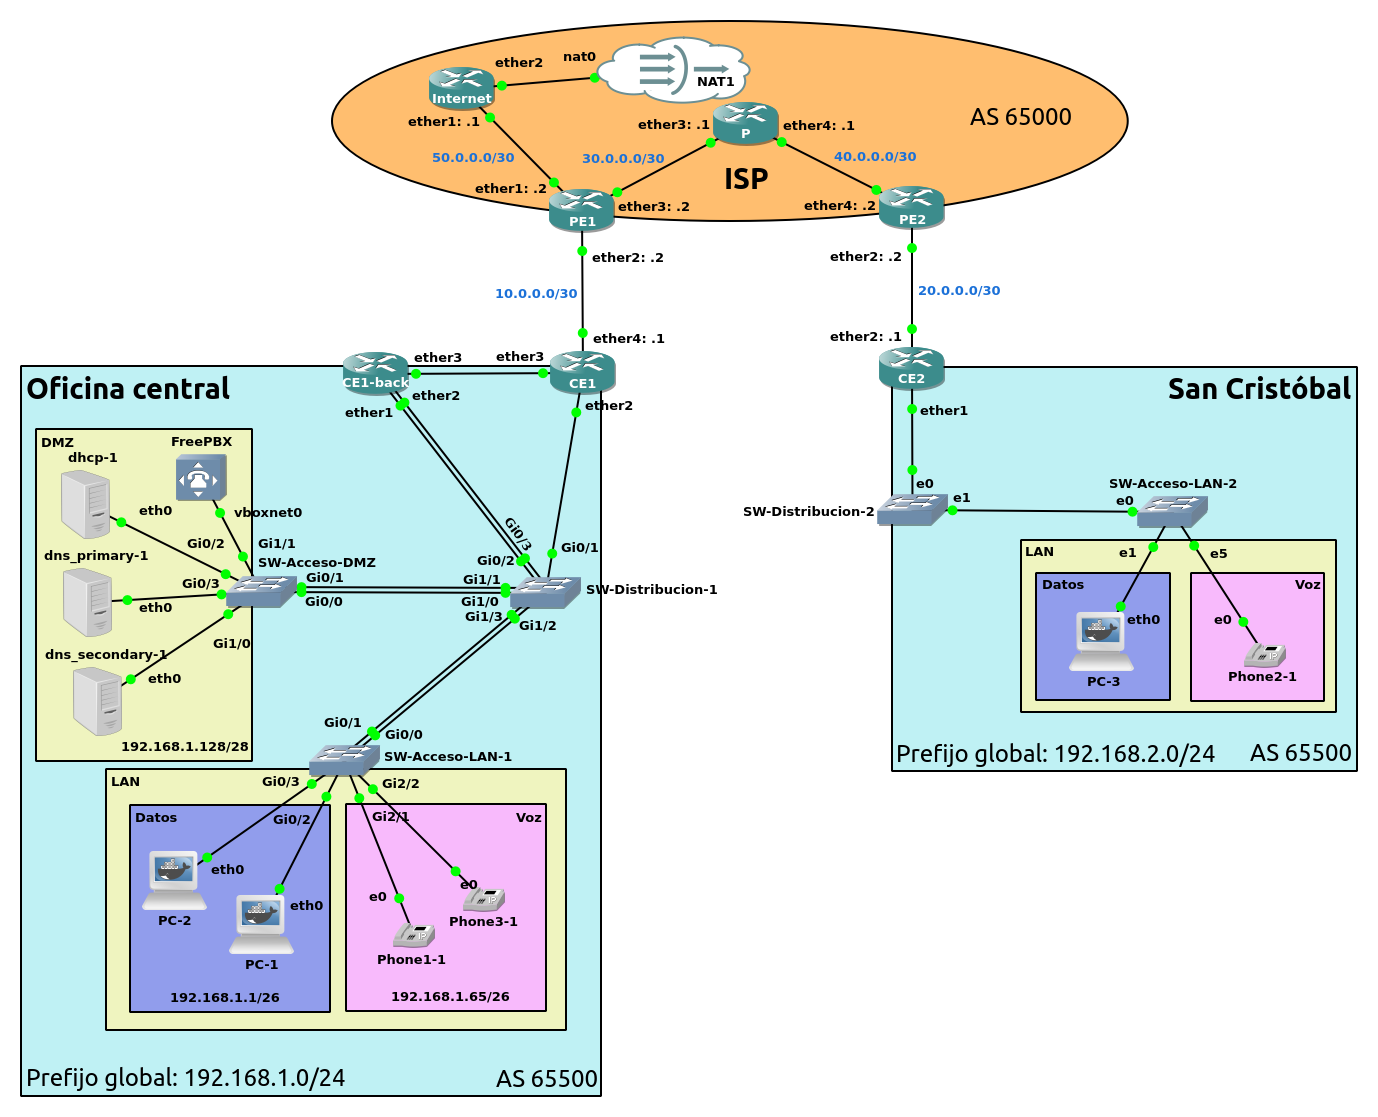
\includegraphics[width=0.9\textwidth]{images/simulacion_entera.png}
	\caption{Simulación de la red completa}
	\label{fig:simulation_office_sancristobal}
\end{figure}

Para la red ISP se ha tomado como referencia la topología L3 MPLS VPN del Trabajo de Fin de Grado de D. Carpio Ortiz
\cite{carpio2023tfg}, adaptándola a los requisitos de la simulación. Se han empleado cuatro routers MikroTik (PE1, PE2, P y un router conectado a una Cloud de GNS3), configurados de forma similar a lo descrito en la sección \ref{sec:simulacion_red_isp}. Además, se ha seguido el esquema de direccionamiento de la Tabla~\ref{tab:tabla_direccionamiento_red_completa} para asignar la red MPLS.

\begin{table}[htb]
	\centering
	\begin{subtable}[b]{0.475\textwidth}
		\centering
		\begin{tabular}{|l|l|l|}
			\hline
			\textbf{Router} & \textbf{Interfaz} & \textbf{Dirección IP} \\ \hline
			CE1             & Lo0               & 192.170.0.1/32        \\ \cline{2-3}
			                & ether1            & 10.0.0.1/30           \\ \cline{2-3}
			                & ether2            & 192.168.1.1/30        \\ \cline{2-3}
			                & ether3            & 10.0.0.14/30          \\ \hline
			PE1             & Lo0               & 192.170.0.2/32        \\ \cline{2-3}
			                & ether1            & 10.0.0.2/30           \\ \cline{2-3}
			                & ether2            & 30.0.0.2/30           \\ \cline{2-3}
			                & ether3            & 50.0.0.1/30           \\ \hline
			P               & Lo0               & 192.170.0.3/32        \\ \cline{2-3}
			                & ether1            & 30.0.0.1/30           \\ \cline{2-3}
			                & ether2            & 40.0.0.1/30           \\ \hline
		\end{tabular}
	\end{subtable}
	\hfill
	\begin{subtable}[b]{0.475\textwidth}
		\centering
		\begin{tabular}{|l|l|l|}
			\hline
			\textbf{Router} & \textbf{Interfaz} & \textbf{Dirección IP} \\ \hline
			PE2             & Lo0               & 192.170.0.4/32        \\ \cline{2-3}
			                & ether1            & 40.0.0.2/30           \\ \cline{2-3}
			                & ether2            & 20.0.0.2/30           \\ \hline
			CE2             & Lo0               & 192.170.0.5/32        \\ \cline{2-3}
			                & ether1            & 20.0.0.1/30           \\ \cline{2-3}
			                & ether2            & 192.168.2.1/30        \\ \hline
			Internet        & Lo0               & 192.170.0.1/32        \\ \cline{2-3}
			                & ether1            & 50.0.0.2/30           \\ \cline{2-3}
			                & ether2            & DHCP                  \\ \hline
		\end{tabular}
	\end{subtable}
	\caption{Esquema de direccionamiento para la red MPLS}
	\label{tab:tabla_direccionamiento_red_completa}
\end{table}

\vspace{0.5cm}
Para completar la simulación, se ha centralizado el acceso a Internet a través de la Oficina Central. De este modo,
todo el tráfico externo generado por los hosts de las sedes remotas (por ejemplo, San Cristóbal) no se dirige directamente fuera de su propia sede, sino que primero es redirigido a la Oficina Central. Allí, el router CE1 actúa como puerta de enlace principal, aplicando NAT al tráfico saliente. La configuración correspondiente en el router CE1 es la siguiente:

\begin{lstlisting}[language=RouterOS]
[admin@CE1] > /ip firewall nat add action=masquerade chain=srcnat dst-address=!192.168.0.0/16 out-interface=ether4
\end{lstlisting}

Esta regla de NAT se aplica a todo el tráfico que sale por la interfaz \texttt{ether4} (que está conectada a la red ISP) y que no tiene como destino una dirección de la red interna (192.168.0.0/16). Esto asegura que todo el tráfico de salida a Internet desde las sedes remotas sea enmascarado con la dirección IP pública del router CE1, permitiendo que los hosts de las sedes remotas puedan acceder a Internet a través de la Oficina Central. Además, se ha añadido una ruta estática para dirigir el tráfico hacia el router PE1 de la red ISP para que pueda salir a Internet.
\begin{lstlisting}[language=RouterOS]
[admin@CE1] > /ip route add gateway=10.0.0.2
\end{lstlisting}

En la Figura~\ref{traceroutePC3} se puede ver el resultado de un \texttt{traceroute} desde un PC en la sede San Cristóbal a un servidor de Google (8.8.8.8) donde se puede observar que el tráfico sale de la LAN de la sede remota, atraviesa el router CE2, luego viaja por la red backbone MPLS (VPN L3) hasta llegar al router CE1 en la Oficina Central, donde se reenvía al router PE1, que es el punto de salida hacia el ISP. Finalmente, el tráfico atraviesa el router de frontera a Internet y accede a la nube (Internet).

\begin{figure}[htb]
	\centering
	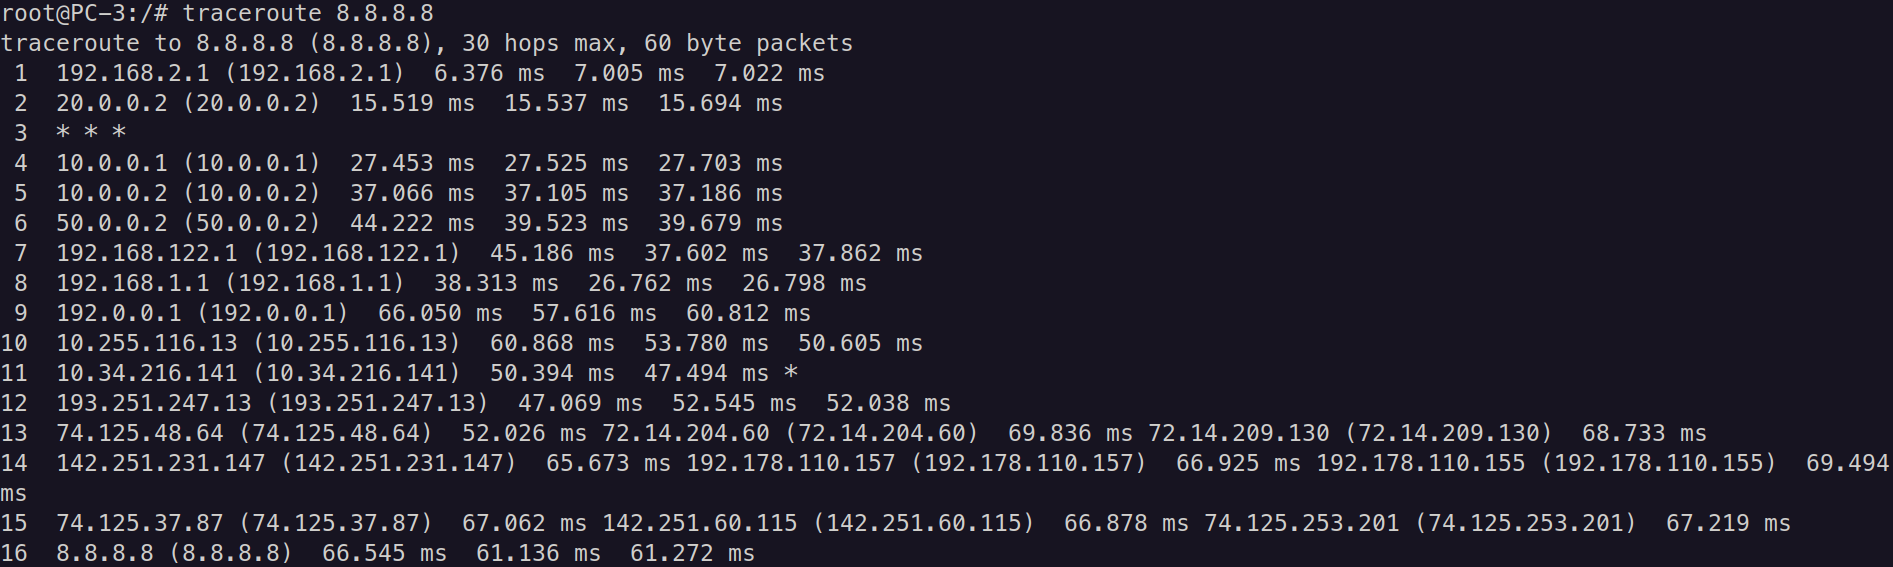
\includegraphics[width=0.95\textwidth]{images/traceroute_PC3_toInternet.png}
	\caption{Resultado de un traceroute desde un PC San Cristóbal a Internet}
	\label{traceroutePC3}
\end{figure}

Por otro lado, las sedes tienen direccionamiento IPv4 para simplificar la simulación ya que los routers MikroTik tienen algunas limitaciones con IPv6, como la falta de soporte para trabajar con MPLS. Por lo tanto, la Oficina Central tendrá una configuración similar a la que se realizó anteriormente, pero con direccionamiento IPv4 con un prefijo \texttt{192.168.1.0/24}. Para los servidores de red, se han creado contenedores Docker personalizados para el servicio DHCP y para el servicio DNS, con una configuración similar a la utilizada en la simulación de la Oficina Central, pero adaptada a direccionamiento IPv4. En los apéndices \ref{Apendice2:configuracion_dhcp_red_completa} y \ref{Apendice2:configuracion_dns_red_completa} se puede consultar la configuración detallada de cada uno de estos servicios. En cuanto a los switches de la Oficina Central, se ha utilizado los de la simulación de la Oficina Central y con la misma configuración.

\vspace{0.5cm}
En cuanto a la sede de San Cristóbal se ha realizado una configuración básica, donde se ha usado un router MikroTik identifiado como CE2 \ref{Apendice2:configuracion_ce2_san_cristobal} con un prefijo \texttt{192.168.2.0/24} y se ha usado switches ethernet de GNS3 para hacer una configuración sencilla de VLANs y conectividad. En la figura \ref{fig:switches_san_cristobal} se puede ver la configuración de los switches de la sede de San Cristóbal.

\begin{figure}[H]
	\centering
	\begin{subfigure}[b]{0.49\textwidth}
		\centering
		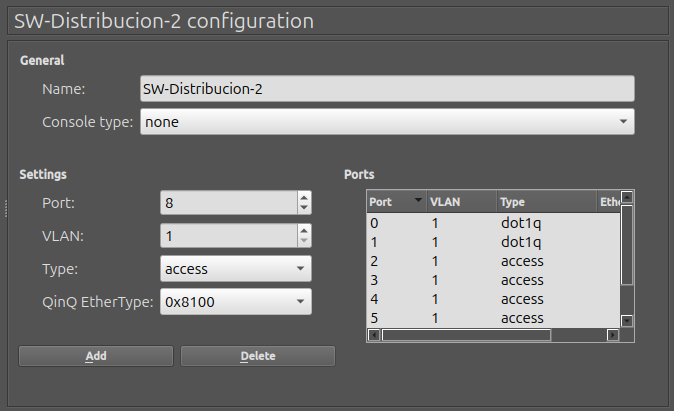
\includegraphics[width=\textwidth]{images/SanCristobal_SW-Distribucion_configuration.png}
		\caption{Switch de distribución de San Cristóbal}
		\label{subfig:switches_san_cristobal_1}
	\end{subfigure}
	\hfill
	\begin{subfigure}[b]{0.49\textwidth}
		\centering
		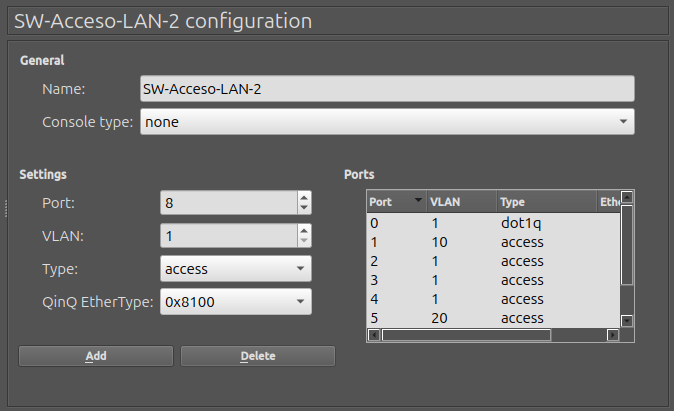
\includegraphics[width=\textwidth]{images/SanCristobal_SW-Acceso_configuration.png}
		\caption{Switch de acceso de San Cristóbal}
		\label{subfig:switches_san_cristobal_2}
	\end{subfigure}
	\caption{Configuración de los switches de la sede de San Cristóbal}
	\label{fig:switches_san_cristobal}
\end{figure}

En esta sede se ha configurado en el propio router CE2 un servidor DHCP (para simplificar la configuracion), que asigna las direcciones IP a los dispositivos de la red. Para ello, se ha creado un pool de direcciones IP para cada VLAN y se ha configurado el servidor para que asigne direcciones IP dentro de estos pools. Además, se ha configurado el gateway para cada VLAN.
\begin{lstlisting}[language=RouterOS]
# Pool de direcciones DHCP
/ip pool add name=pool_datos ranges=192.168.2.2-192.168.2.30
/ip pool add name=pool_voz ranges=192.168.2.34-192.168.2.62

# Servidor DHCP para VLAN 10 (Datos)
/ip dhcp-server add name=dhcp_datos interface=vlan10-datos address-pool=pool_datos disabled=no
/ip dhcp-server network add address=192.168.2.0/26 gateway=192.168.2.1

# Servidor DHCP para VLAN 20 (Voz)
/ip dhcp-server add name=dhcp_voz interface=vlan20-voz address-pool=pool_voz disabled=no
/ip dhcp-server network add address=192.168.2.32/26 gateway=192.168.2.33
\end{lstlisting}

Por último, para la conectividad de los dispositivos finales, se han creado contenedores Docker personalizados que actúan como PCs de prueba, parecidos a los utilizados en la Oficina Central pero para funcionar en IPv4. Además, como softphone se ha usado una máquina virtual ligera que viene instalada con algunas aplicaciones VoIP, obtenida de un tutorial de \texttt{Youtube} de C. E. Carrillo Arellano \cite{youtube_carlos_carrillo}. En esta máquina virtual viene instalado algunos softphones como \texttt{Zoiper} y \texttt{Microsip} y se ha configurado para que se pueda usar en la VLAN de voz. Para la centralita de telefonía IP se ha instalado \texttt{FreePBX} en una máquina virtual en \texttt{VirtualBox} y se ha configurado con una IP estática \texttt{192.168.1.135} y se ha conectado en la DMZ de la Oficina Central. Para simplificar la configuración, esta centralita se ha configurado para que pueda gestionar las llamadas entre los teléfonos IP de la Oficina Central y se han creado dos extensiones para comprobar la comunicación entre
los teléfonos IP de esta sede. En la Figura~\ref{fig:test_voip_ipv4} se puede ver la comprobación de la VoIP, donde se puede ver que se ha realizado una llamada entre dos teléfonos IP y se ha establecido la comunicación correctamente.

\begin{figure}[H]
	\centering
	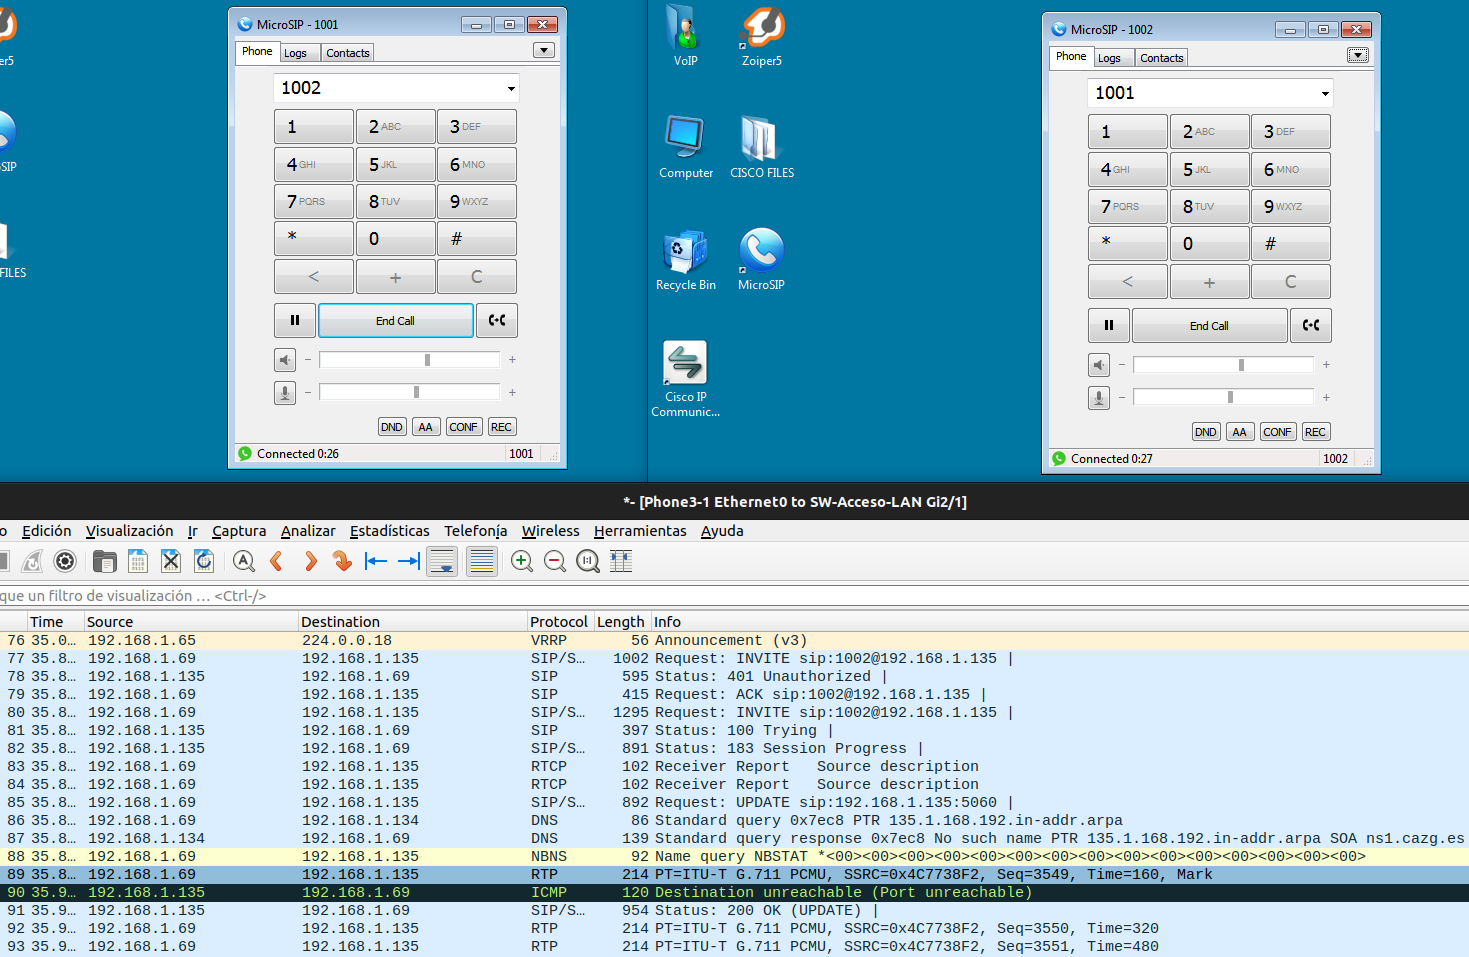
\includegraphics[width=0.8\textwidth]{images/test_voip_ipv4.png}
	\caption{Comprobación de la VoIP sobre IPv4}
	\label{fig:test_voip_ipv4}
\end{figure}

\section{Laboratorio}
En esta sección se describe la prueba que se realizó en el laboratorio efectuada para comprobar la comunicación entre dos teléfonos IP utilizando dispositivos físicos. Para ello, se emplearon un router \texttt{MikroTik RB2011UiAS-RM}, switches \texttt{TP-Link T2500G-10TS} y teléfonos IP \texttt{Grandstream GRP2601}. Los servicios de red DHCP y DNS se implementaron de forma simulada mediante GNS3 y se han usado los mismos contenedores que se han usado para las simulación de la red completa \ref{sec:simulacion_completa}. Estos contendores se estarán ejecutando en un ordenador físico (PC1) del laboratorio siguiendo el esquema de la Figura~\ref{fig:servicios_red_laboratorio}.

\begin{figure}[H]
	\centering
	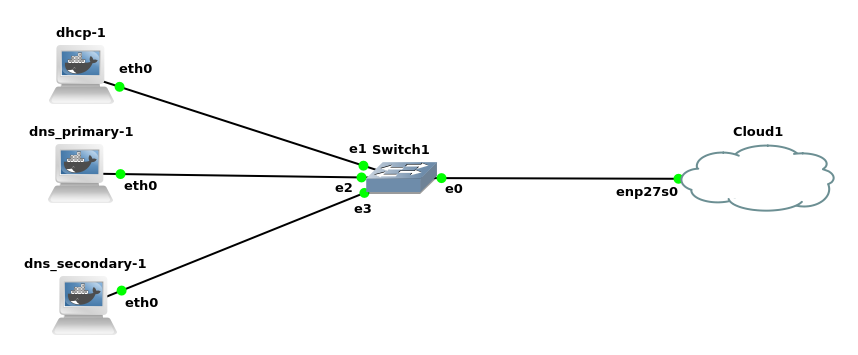
\includegraphics[width=0.75\textwidth]{images/servicios_red_laboratorio.png}
	\caption{Servicios de red utilizados en el laboratorio}
	\label{fig:servicios_red_laboratorio}
\end{figure}

Además, se ha usado otro ordenador físico (PC2) para operar como la centralita FreePBX y se ha ejecutado un contenedor Docker con
la imagen de FreePBX, y en este PC se ha configurado con una IP estática \texttt{192.168.1.135}. El docker-compose para la centralita
que se ha usado se encuentra en el apéndice \ref{Apendice2:docker_compose_freepbx}. En la Figura~\ref{fig:interconexion_red_laboratorio} se muestra
la interconexión que se ha realizado en el laboratorio.
\begin{figure}[H]
	\centering
	\begin{subfigure}[b]{0.59\textwidth}
		\centering
		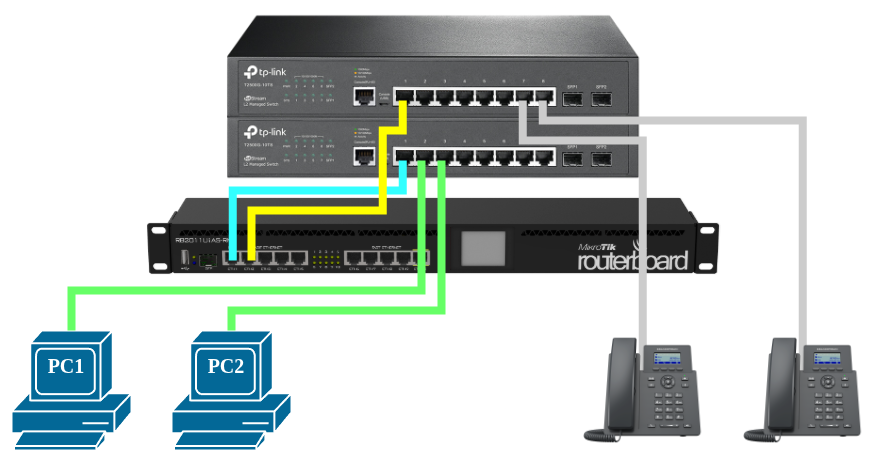
\includegraphics[width=\textwidth]{images/interconexion_red_laboratorio.png}
		\caption{Interconexión de los dispositivos}
		\label{fig:interconexion_red}
	\end{subfigure}
	\hfill
	\begin{subfigure}[b]{0.39\textwidth}
		\centering
		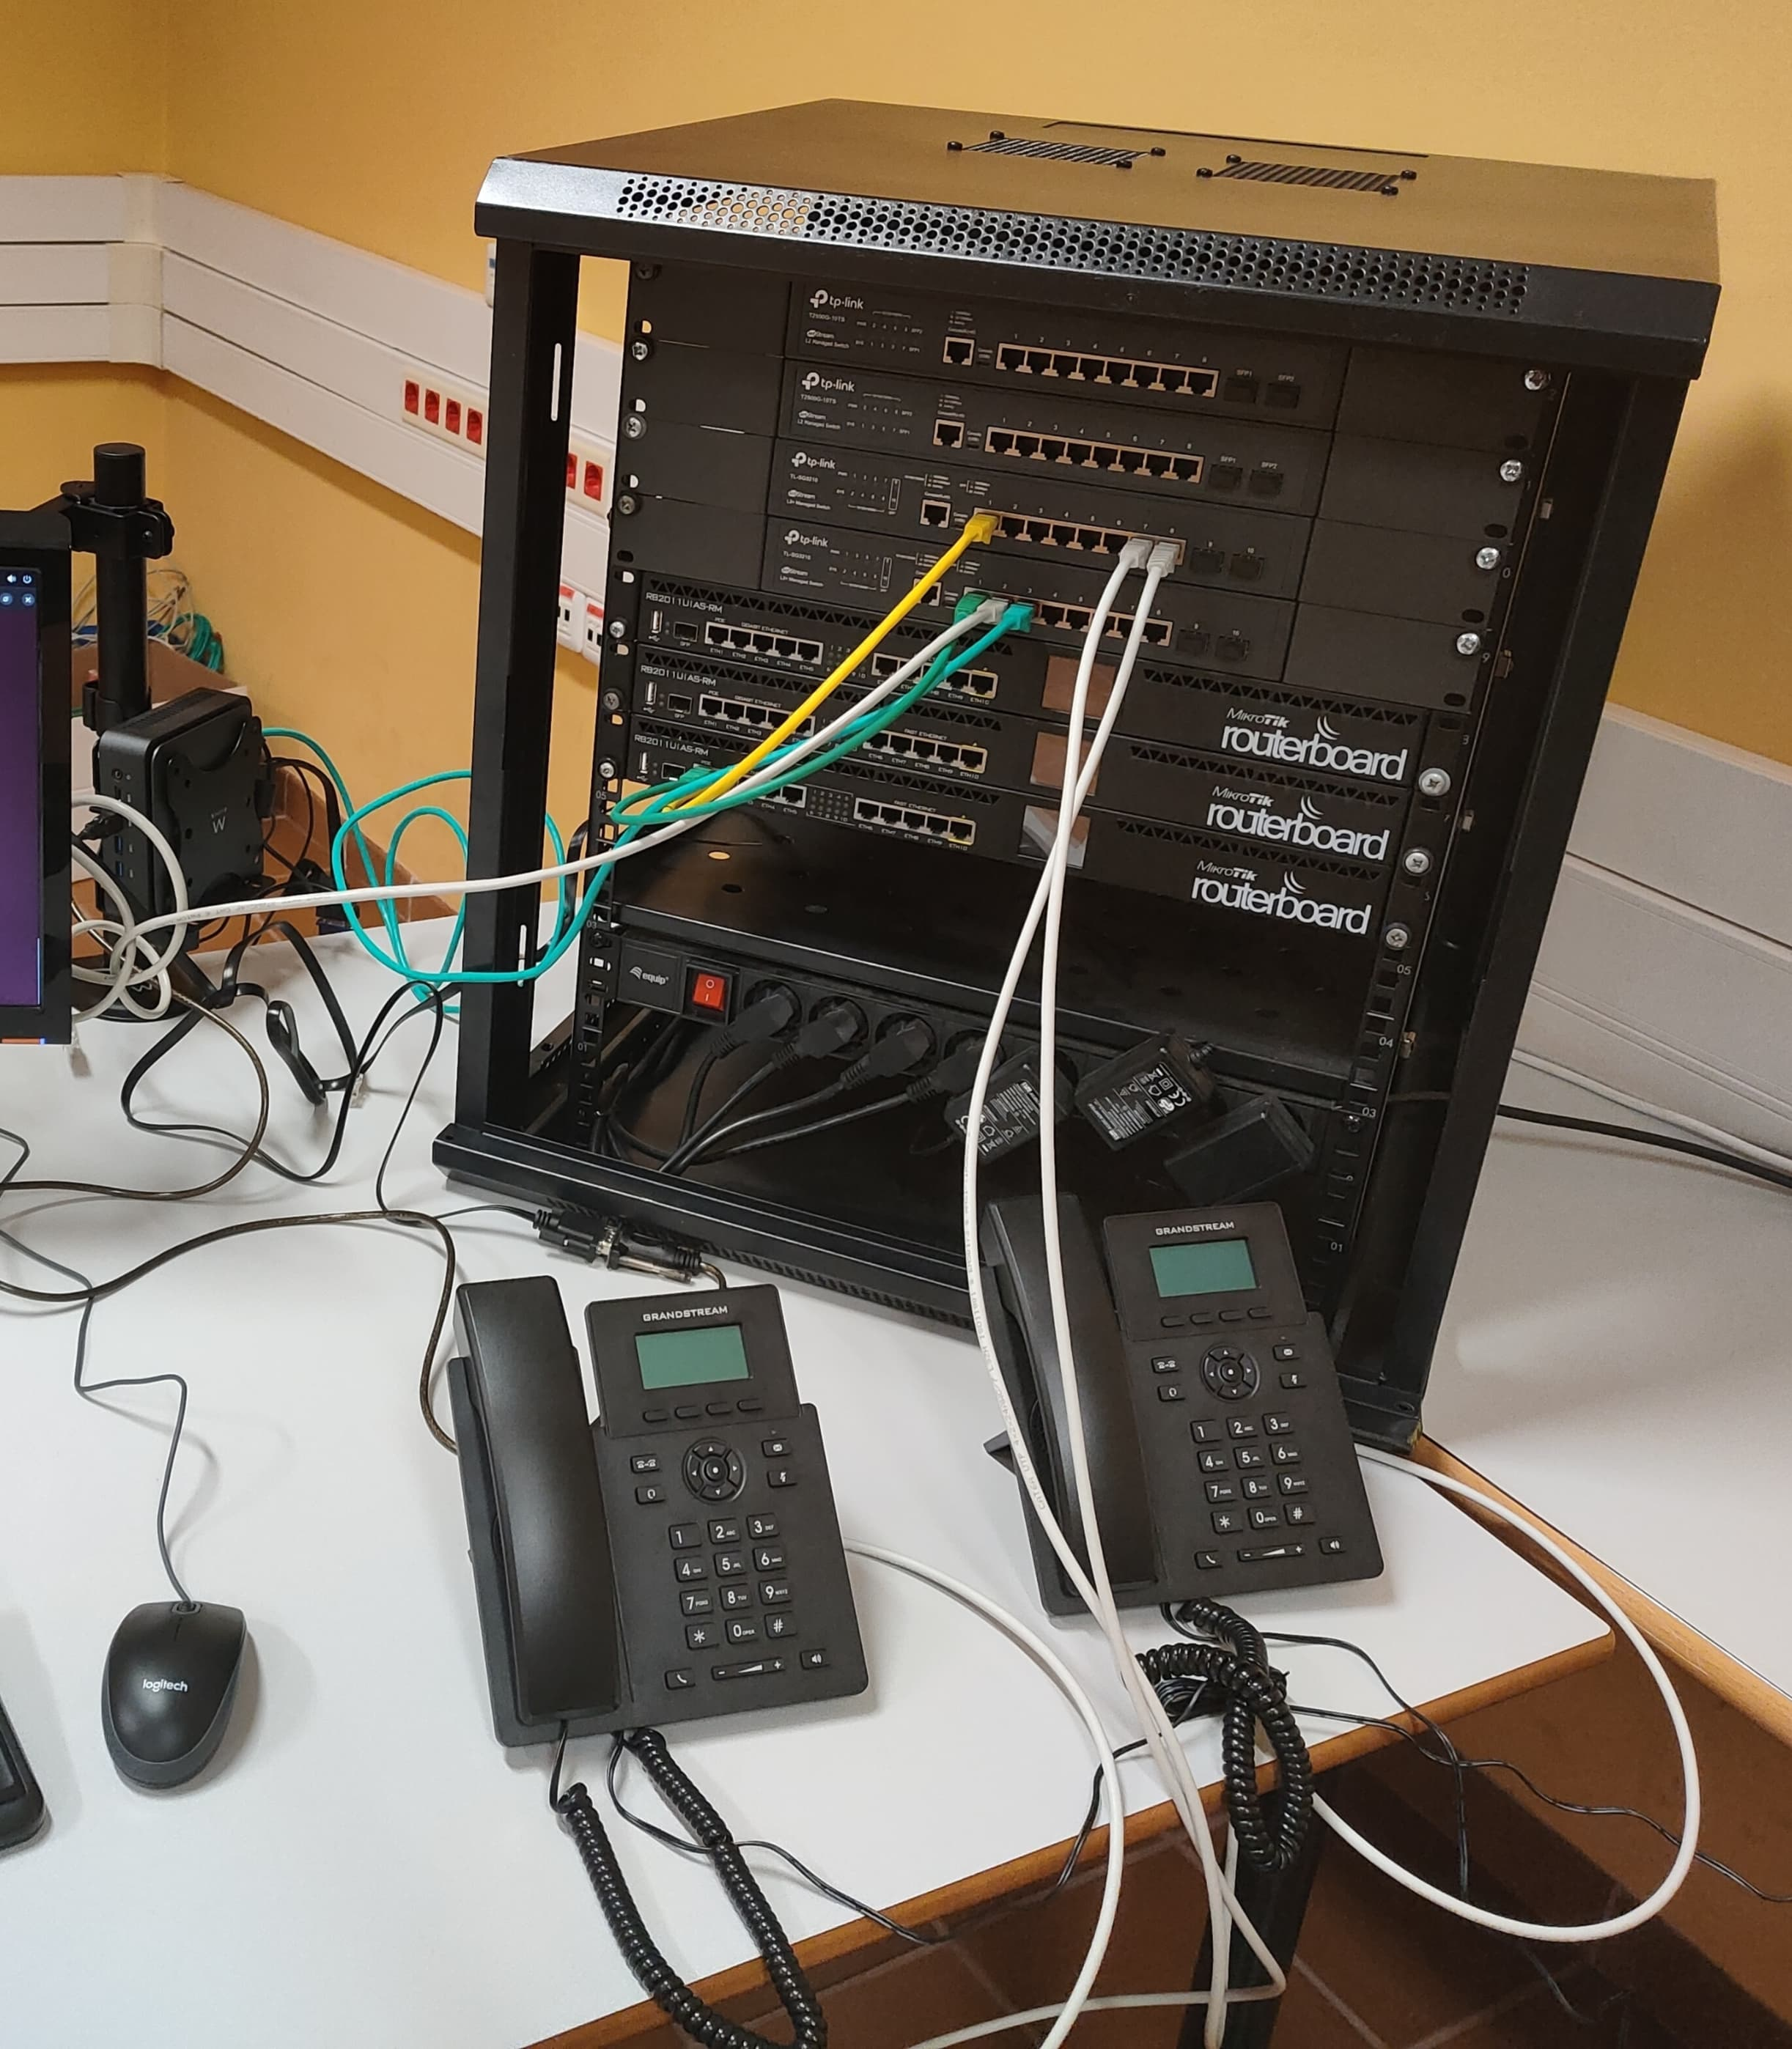
\includegraphics[width=\textwidth]{images/laboratorio.jpeg}
		\caption{Dispositivos físicos del laboratorio}
		\label{fig:laboratorio}
	\end{subfigure}
	\caption{Interconexión de red y dispositivos físicos utilizados en el laboratorio}
	\label{fig:interconexion_red_laboratorio}
\end{figure}

Por otro lado, en la centralita FreePBX se han creado dos extensiones, 1001 y 1002, destinadas al uso con teléfonos
IP, como se muestra en la Figura~\ref{fig:extensiones_telefonoIP}. Estas extensiones permiten realizar y recibir
llamadas dentro de la red local del sistema de telefonía.

\begin{figure}[H]
	\centering
	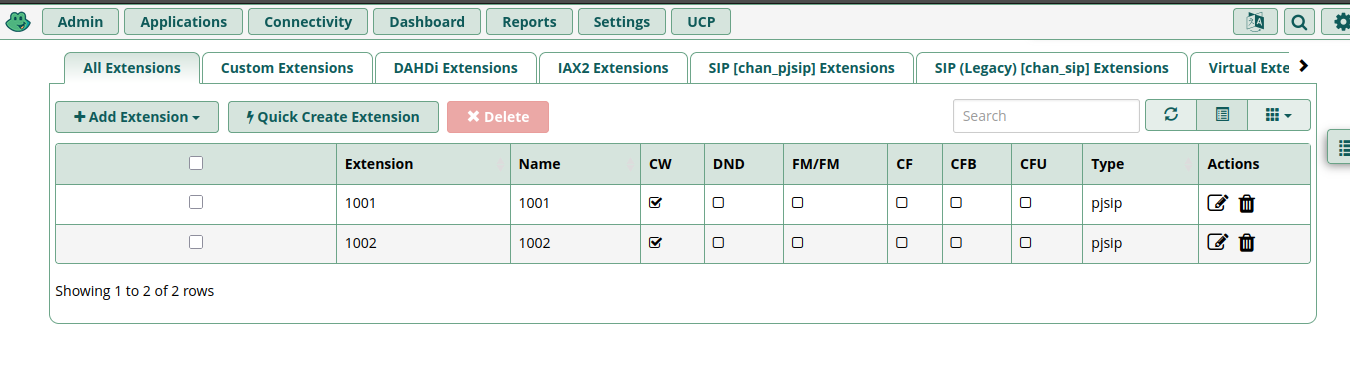
\includegraphics[width=1\textwidth]{images/extensiones_telefonoIP.png}
	\caption{Extensiones configuradas en la centralita FreePBX}
	\label{fig:extensiones_telefonoIP}
\end{figure}

Para cada una de estas extensiones se ha configurado un buzón de voz, permitiendo que los usuarios dejen mensajes
cuando no se puede atender una llamada. Esta funcionalidad resulta especialmente útil en entornos donde no siempre
es posible responder inmediatamente. En la Figura~\ref{fig:configuracion_buzon_voz} se muestra un ejemplo de esta
configuración, correspondiente a la extensión 1001. Entre las opciones disponibles se encuentran la definición de
la contraseña del buzón, el envío de mensajes por correo electrónico, y la posibilidad de reproducir el
identificador de llamada (CID) y los datos del mensaje (fecha y hora).

\begin{figure}[H]
	\centering
	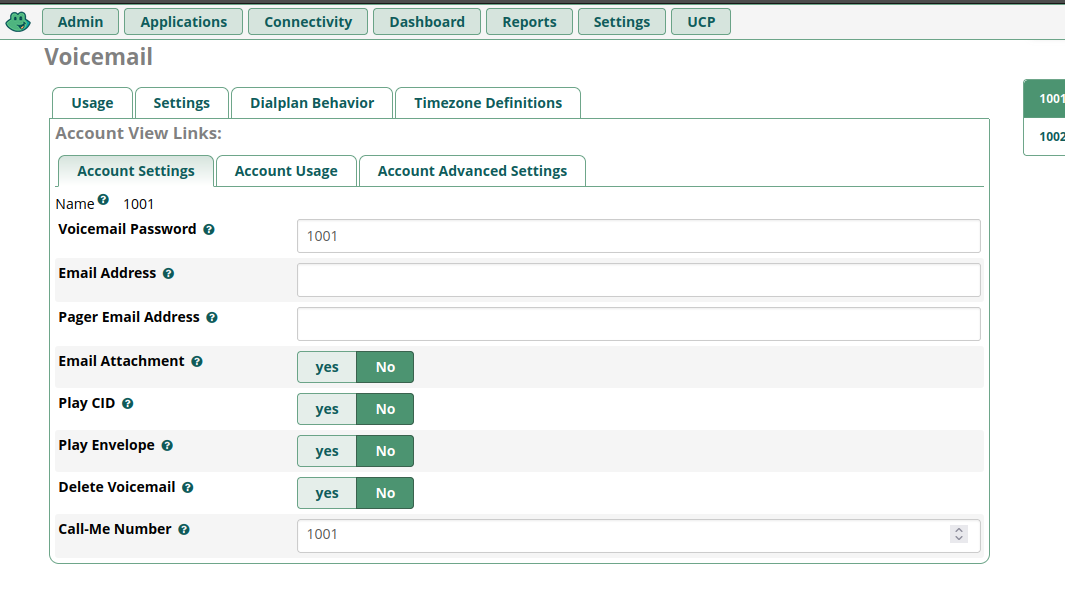
\includegraphics[width=0.8\textwidth]{images/configuracion_buzon_voz.png}
	\caption{Configuración del buzón de voz para la extensión 1001}
	\label{fig:configuracion_buzon_voz}
\end{figure}

Por último, los dispositivos conectados a la red obtienen sus direcciones IP mediante el protocolo DHCP,
el cual se encuentra ejecutándose en el ordenador físico (PC1) del laboratorio.


%%%%%%%%%%%%%%%%%%%%%%%%%%%%%%%%%%%%%%%%%%%%%%%%%%%%%%%%%

%%%%%%%%%%%%%%%%%%%%%%%%%%%%%%%%%%%%%%%%%%%%%%%%%%%%%%%%%%
\newpage
\thispagestyle{empty}
\vspace*{\fill}
\begin{center}
  % Página intencionadamente en blanco
\end{center}
\vspace*{\fill}
\newpage
%%%%%%%%%%%%%%%%%%%%%%%%%%%%%%%%%%%%%%%%%%%%%%%%%%%%%%%%%%


\newpage{\pagestyle{empty}}
\thispagestyle{empty}

\chapter{\LARGE Conclusiones y líneas futuras}
\label{chapter:conclusiones}

El presente Trabajo de Fin de Grado ha permitido diseñar una infraestructura de red moderna y escalable cogiendo de referencia el pliego de proyectos del Consorcio de Aguas de la Zona Gaditana, centrada en la mejora de la conectividad, la seguridad y la integración de servicios en sus distintas sedes. A través del uso de tecnologías como \texttt{SD-WAN}, direccionamiento IPv6, telefonía IP y cortafuegos de nueva generación.

\vspace{0.5cm}
Durante el desarrollo del proyecto se ha realizado un análisis detallado de los requisitos técnicos y se ha diseñado una topología en estrella con una arquitectura de red jerárquica de tres capas (núcleo, distribución y acceso). Además, se han seleccionado los dispositivos de red, teniendo en cuenta su rendimiento, escalabilidad, compatibilidad y coste.

\vspace{0.5cm}
La simulación de la red mediante \texttt{GNS3} ha servido para validar parcialmente el diseño propuesto, a pesar de las limitaciones técnicas de la herramienta frente a entornos reales basados en soluciones como \texttt{Cisco Meraki}. 

\vspace{0.5cm}
A partir del trabajo realizado, se proponen las siguientes líneas de trabajo que pueden servir para mejorar el desarrollo y evolución del proyecto:
\begin{itemize}
  \item \textbf{Implantación de sistemas en la nube:} implementar la centralita \texttt{FreePBX} en la plataforma \texttt{Microsoft Azure}, aprovechando la escalabilidad y disponibilidad que ofrece la nube. Además, se recomienda integrar \texttt{Microsoft Sentinel} como plataforma de respuesta ante incidentes, permitiendo la monitorización, detección y gestión centralizada de amenazas y eventos de seguridad relacionados con la telefonía IP y otros servicios críticos.

  \item \textbf{Automatización de la configuración de red:} usar herramientas como \texttt{Ansible} o scripts \texttt{Python} para automatizar el despliegue y configuración de routers y switches en la simulación.

  \item \textbf{Automatización y monitorización avanzada:} desplegar herramientas de monitorización complementarias como \texttt{Zabbix} para lograr una supervisión más detallada de los servicios y dispositivos no gestionados por \texttt{Meraki}.

  \item \textbf{Evaluación del rendimiento simulado y mejora continua:} realizar pruebas de estrés, análisis de tráfico y simulaciones de escenarios críticos en entornos virtuales como \texttt{GNS3}, con el objetivo de validar el diseño propuesto, optimizar su comportamiento teórico y detectar posibles debilidades en la arquitectura de red.
\end{itemize}

%%%%%%%%%%%%%%%%%%%%%%%%%%%%%%%%%%%%%%%%%%%%%%%%%%%%%%%%%

%%%%%%%%%%%%%%%%%%%%%%%%%%%%%%%%%%%%%%%%%%%%%%%%%%%%%%%%%%
\newpage
\thispagestyle{empty}
\vspace*{\fill}
\begin{center}
  % Página intencionadamente en blanco
\end{center}
\vspace*{\fill}
\newpage
%%%%%%%%%%%%%%%%%%%%%%%%%%%%%%%%%%%%%%%%%%%%%%%%%%%%%%%%%%

\newpage{\pagestyle{empty}}
\thispagestyle{empty}

\chapter{\LARGE Summary and Conclusions}
\label{chapter:conclusions}

This Final Degree Project has enabled the design of a modern and scalable network infrastructure based on the project specifications of the Consorcio de Aguas de la Zona Gaditana, focused on improving connectivity, security and the integration of services at its various sites. Through the use of technologies such as \texttt{SD-WAN}, IPv6 addressing, IP telephony and new generation firewalls.

\vspace{0.5cm}
During the development of the project, a detailed analysis of the technical requirements has been carried out and a star topology has been designed with a hierarchical network architecture of three layers (core, distribution and access). In addition, network devices have been selected, taking into account their performance, scalability, compatibility and cost.

\vspace{0.5cm}
The simulation of the network using \texttt{GNS3} has served to partially validate the proposed design, despite the technical limitations of the tool compared to real environments based on solutions such as \texttt{Cisco Meraki}.

\vspace{0.5cm}
Based on the work carried out, the following lines of work are proposed that can be used to improve the development and evolution of the project:
\begin{itemize}
  \item \textbf{Implementation of systems in the cloud:} implement the \texttt{FreePBX} PBX on the \texttt{Microsoft Azure} platform, taking advantage of the scalability and availability offered by the cloud. In addition, it is recommended to integrate  \texttt{Microsoft Sentinel} as an incident response platform, enabling centralised monitoring, detection and management of threats and security events related to IP telephony and other critical services.

  \item \textbf{Network configuration automation:} use tools such as \texttt{Ansible} or \texttt{Python} scripts to automate the deployment and configuration of routers and switches in the simulation.

  \item \textbf{Automation and advanced monitoring:} deploy complementary monitoring tools such as \texttt{Zabbix} for more detailed monitoring of services and devices not managed by \texttt{Meraki}.

  \item \textbf{Simulated performance evaluation and continuous improvement:} perform stress tests, traffic analysis and simulations of critical scenarios in virtual environments such as \texttt{GNS3}, in order to validate the proposed design, optimise its theoretical behaviour and detect possible weaknesses in the network architecture.
\end{itemize}

%%%%%%%%%%%%%%%%%%%%%%%%%%%%%%%%%%%%%%%%%%%%%%%%%%%%%%%%%

%%%%%%%%%%%%%%%%%%%%%%%%%%%%%%%%%%%%%%%%%%%%%%%%%%%%%%%%%%
\newpage
\thispagestyle{empty}
\vspace*{\fill}
\begin{center}
  % Página intencionadamente en blanco
\end{center}
\vspace*{\fill}
\newpage
%%%%%%%%%%%%%%%%%%%%%%%%%%%%%%%%%%%%%%%%%%%%%%%%%%%%%%%%%%

\newpage{\pagestyle{empty}}
\thispagestyle{empty}

\chapter{\LARGE Presupuesto}
\label{chapter:presupuesto}
En este capítulo se detalla los costes asociados al desarrollo del proyecto, incluyendo el tiempo estimado para cada tarea y el coste total del proyecto. Por lo que se refiere a gastos de hardware, software o licencias, no se han considerado ya que el proyecto se ha desarrollado utilizando herramientas de código abierto y simuladores que no requieren licencias. En cuanto al hardware utilizado, es el equipo personal que ya estaba disponible antes del inicio del proyecto.

\section{Costes del proyecto}
Para calcular los costes de personal, se ha considerado un salario anual de 28.000 euros brutos para un Ingeniero Informático Junior en España, con lo que el coste por hora sería de aproximadamente 15 euros brutos. Para el desarrollo del proyecto, se ha estimado un total de 300 horas de trabajo distribuidas en las siguientes tareas:
\begin{table}[H]
	\centering
	\small
	\begin{tabular}{|l|c|r|}
		\hline
		\textbf{Tarea}                   & \textbf{Horas estimadas} & \textbf{Coste estimado (euros)} \\
		\hline
		Investigación preliminar         & 20                       & 150 €                           \\ \hline
		Análisis de requisitos           & 20                       & 300 €                           \\ \hline
		Diseño de la red                 & 40                       & 600 €                           \\ \hline
		Selección de hardware y software & 20                       & 300 €                           \\ \hline
		Implementación en simuladores    & 100                      & 1500 €                          \\ \hline
		Pruebas y ajustes                & 50                       & 750 €                           \\ \hline
		Redacción de la memoria          & 50                       & 600 €                           \\ \hline
		\textbf{Total}                   & \textbf{300}             & \textbf{4200 €}                 \\
		\hline
	\end{tabular}
	\caption{Costes de personal}
	\label{tab:costes_proyecto}
\end{table}
El coste total del proyecto se muestra en la tabla \ref{tab:presupuesto}.
\begin{table}[H]
	\centering
	\small
	\begin{tabular}{|l|c|r|}
		\hline
		\textbf{Partida}                     & \textbf{Coste (euros)} \\
		\hline
		Licencias de software                & 0 €                    \\ \hline
		Amortización de equipos informáticos & 72 €                   \\ \hline
		Costes de personal                   & 4200 €                 \\ \hline
		Otros gastos                         & 50 €                   \\ \hline \hline
		Subtotal                             & 4322 €                 \\ \hline
		IGIC                                 & 302,54 €               \\ \hline \hline
		\textbf{Total}                       & \textbf{4624,54 €}     \\
		\hline
	\end{tabular}
	\caption{Presupuesto.}
	\label{tab:presupuesto}
\end{table}


%%%%%%%%%%%%%%%%%%%%%%%%%%%%%%%%%%%%%%%%%%%%%%%%%%%%%%%%%%
\newpage
\thispagestyle{empty}
\vspace*{\fill}
\begin{center}
  % Página intencionadamente en blanco
\end{center}
\vspace*{\fill}
\newpage
%%%%%%%%%%%%%%%%%%%%%%%%%%%%%%%%%%%%%%%%%%%%%%%%%%%%%%%%%%

%%%%%%%%%%%%%%%%%%%%%%%%%%%%%%%%%%%%%%%%%%%%%%%%%%%%%%%%%
\newpage{\pagestyle{empty}\cleardoublepage}
\thispagestyle{empty}

\begin{appendix}

	\chapter{\LARGE Instalación de programas necesarios}
	\label{appendix:1}
	La instalación de los programas necesarios para el desarrollo de este Trabajo de Fin de Grado se ha realizado en un equipo con Ubuntu 22.04 LTS. Las características hardware del equipo son las siguientes:

\begin{multicols}{2}
\begin{itemize}
    \item Procesador: AMD Ryzen 5 2600 Six-Core @ 12x 3,4GHz
    \item Tarjeta gráfica: NVIDIA GeForce RTX 2060
    \item Memoria RAM: 16 GB
    \item 256 GB SSD
    \item Sistema operativo: Ubuntu 22.04 LTS
\end{itemize}
\end{multicols}

\section{Instalación y configuración de GNS3}
\label{Apendice1:instalacion_gns3}
\noindent
Para instalar GNS3 se va a utilizar el gestor de paquetes de Ubuntu, \texttt{apt}.

\begin{lstlisting}[language=bash]
sudo add-apt-repository ppa:gns3/ppa
sudo apt update
sudo apt install gns3-gui gns3-server
\end{lstlisting}

\noindent
Una vez instalado GNS3 se comprobará que se ha instalado correctamente ejecutando el siguiente comando:

\begin{lstlisting}[language=bash]
gns3 --version
\end{lstlisting}

\noindent
y así se comprobará que se ha instalado correctamente. En este caso, la versión que se ha usado es la 2.2.54. Por otro lado, GNS3 permite la integración de imágenes QEMU/KVM para emular dispositivos de red. Para ello, es recomendable 
contar con soporte para \textbf{KVM} habilitado en el sistema. Esto mejora el rendimiento de las máquinas 
virtuales dentro de GNS3. Para hacer esta comprobación se va a utilizar el paquete \texttt{cpu-checker}. La 
instalación del mismo se hace con:

\begin{lstlisting}[language=bash]
sudo apt install cpu-checker
\end{lstlisting}

\noindent
Una vez instalado el paquete, se puede comprobar si el sistema tiene soporte para KVM ejecutando \lstinline|kvm-ok|:

\begin{lstlisting}[language=bash]
INFO: /dev/kvm exists
KVM acceleration can be used
\end{lstlisting}

\noindent
El resultado debería ser el que se muestra en pantalla. Si no es así, se debe habilitar la virtualización por hardware o que esté desactivada en label BIOS. 

\vspace{1em}
\noindent
Para que todo funcione correctamente, se debe modificar los permisos del ejecutable \texttt{ubridge} para 
que pueda ser ejecutado por el usuario que ejecuta GNS3.

\begin{lstlisting}[language=bash]
sudo chmod 755 /usr/bin/ubridge
\end{lstlisting}

\noindent
Además, para poder hacer uso de las máquinas virtuales dentro del simulador hay que hacer funcionar KVM. La instalación de este componente se debió hacer al instalar GNS3.
Sin embargo, para tener los permisos necesarios debemos añadir el usuario que ejecuta GNS3 al grupo \texttt{kvm}.

\begin{lstlisting}[language=bash]
sudo adduser $USER kvm
\end{lstlisting}

\noindent
Una vez hecho esto, se debe reiniciar el sistema para que los cambios surtan efecto. Una vez reiniciado el sistema, se puede iniciar GNS3 y comprobar que todo funciona correctamente.

\section{Instalación de VirtualBox}
\label{Apendice1:instalacion_virtualbox}
Para instalar VirtualBox \cite{virtualbox} se debe descargar el paquete de instalación desde la página oficial de VirtualBox para la versión del sistema operativo que se esté usando. En este caso, se está usando Ubuntu 22.04 LTS, por lo que se debe descargar el paquete de instalación para esta versión.

\begin{figure}[H]
	\centering
	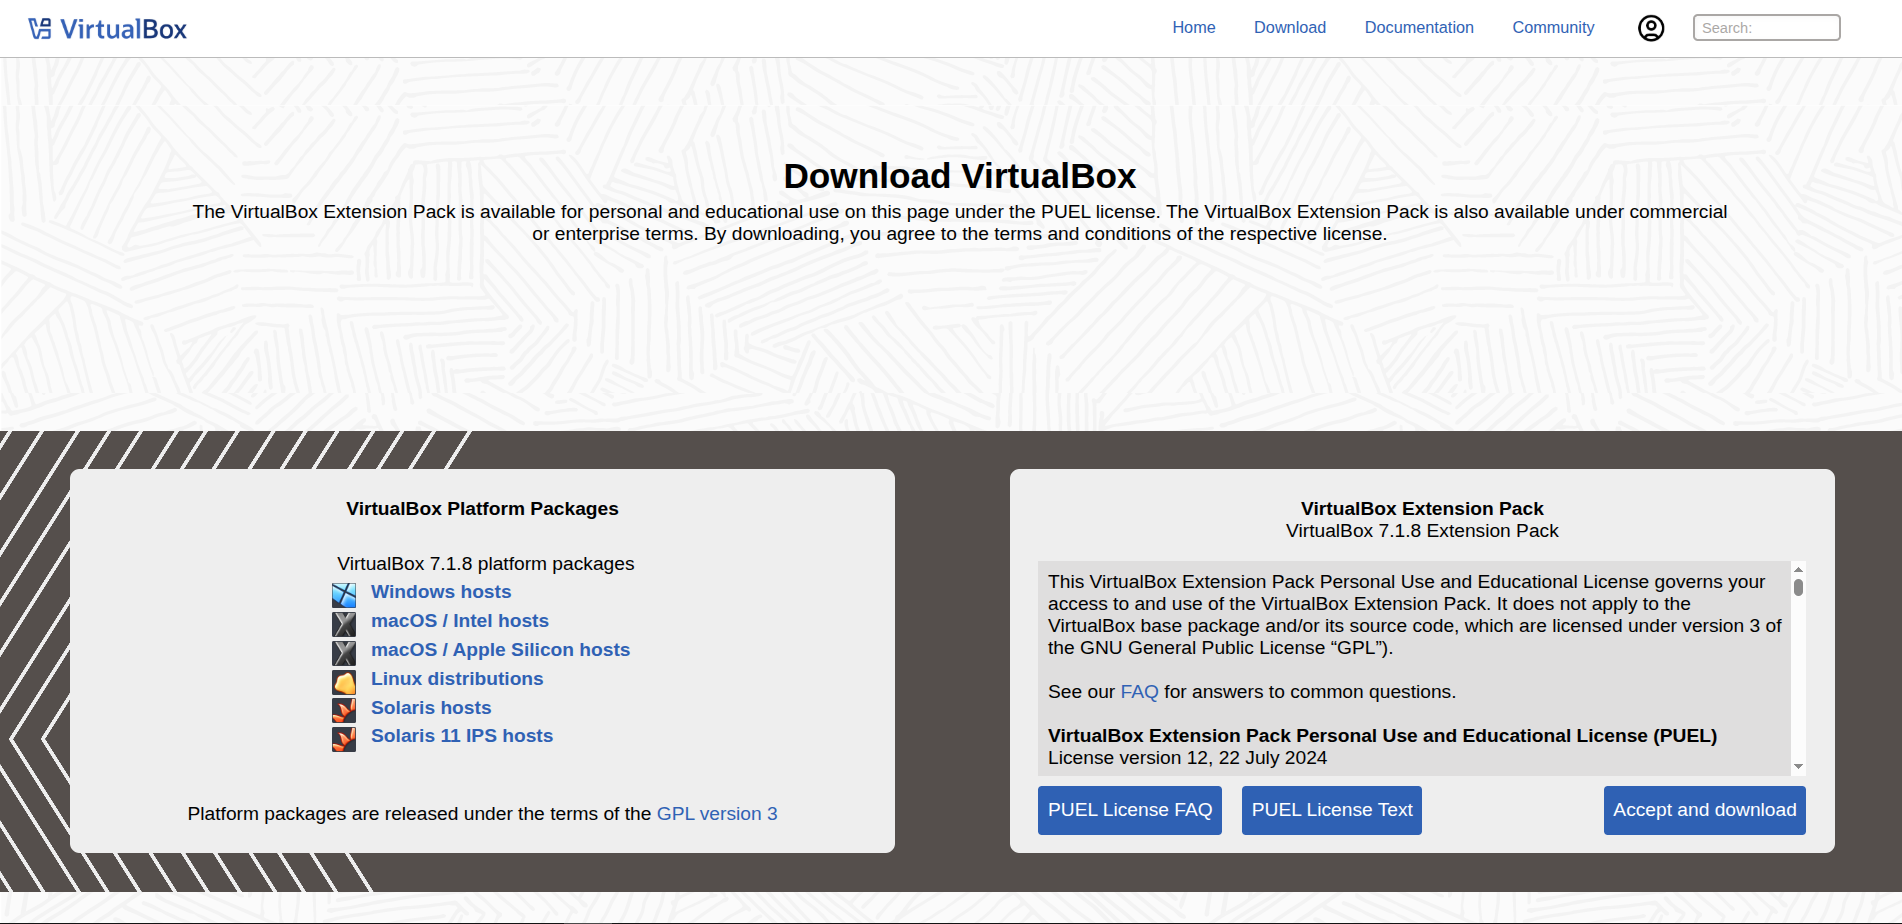
\includegraphics[width=1\textwidth]{images/virtualbox_download.png}
	\caption{Descarga de VirtualBox}
	\label{fig:virtualbox_download}
\end{figure}

\noindent
Elegimos la opción de \texttt{Download VirtualBox for Linux hosts}, en este caso, y elegimos la distribución de Linux que se esté usando. En este caso, se está usando Ubuntu 22.04 LTS, por lo que se debe elegir la opción de \texttt{Ubuntu 22.04 (64-bit)}.

\begin{figure}[H]
	\centering
	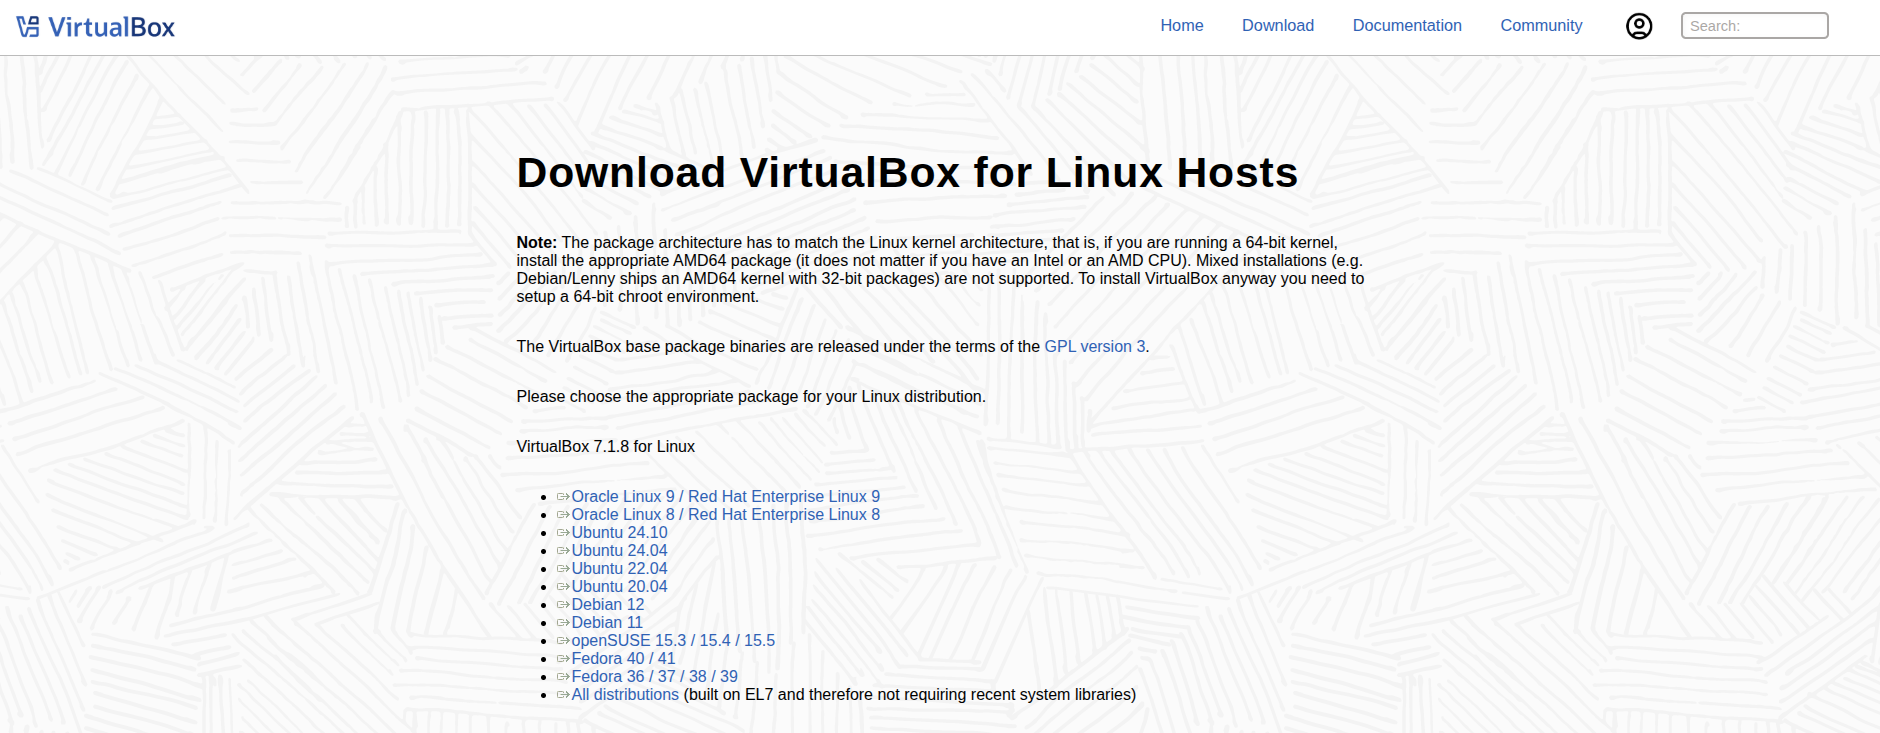
\includegraphics[width=0.9\textwidth]{images/virtualbox_download_2.png}
	\caption{Descarga de VirtualBox}
	\label{fig:virtualbox_download_2}
\end{figure}

\noindent
Una vez descargado el paquete, se debe instalar. Para ello, se debe abrir una terminal y navegar hasta la carpeta donde se ha descargado el paquete.
\begin{lstlisting}[language=bash]
cd ~/Descargas
sudo dpkg -i virtualbox-7.1_7.1.8-168469~Ubuntu~jammy_amd64.deb
\end{lstlisting}

\noindent
Si se produce algún error de dependencias, se puede solucionar ejecutando el siguiente comando:
\begin{lstlisting}[language=bash]
sudo apt --fix-broken install
\end{lstlisting}

\noindent
Una vez instalado VirtualBox, se puede comprobar que se ha instalado correctamente ejecutando el siguiente comando:
\begin{lstlisting}[language=bash]
virtualbox --help
\end{lstlisting}

\noindent
y así se comprobará que se ha instalado correctamente. En este caso, la versión que se ha usado es la 7.1.8.

\subsection{Instalación FreePBX}
\label{Apendice1:instalacion_freepbx}
Para instalar FreePBX \cite{freepbx}, primero es necesario acceder a la página oficial y descargar el instalador correspondiente a la versión del sistema operativo que se esté utilizando. En la sección \texttt{Download}, se debe desplegar la opción \texttt{View Previous Versions} para seleccionar la versión deseada. En este caso, se ha descargado la imagen ISO de la versión \texttt{SNG7-PBX16-64bit-2302-1}, como se muestra en la figura~\ref{fig:freepbx_download}.
\begin{figure}[H]
	\centering
	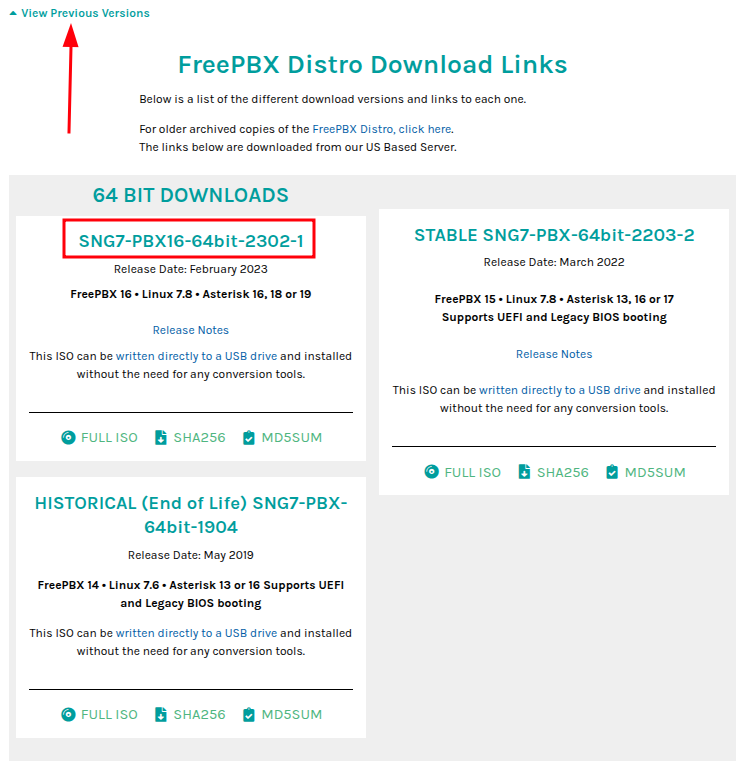
\includegraphics[width=0.7\textwidth]{images/freepbx_download.png}
	\caption{Descarga de FreePBX}
	\label{fig:freepbx_download}
\end{figure}

\vspace{1em}
\noindent
Una vez descargado el paquete, se debe montar la imagen ISO en una máquina virtual de VirtualBox.
Para ello, se debe crear una nueva máquina virtual en VirtualBox, seleccionamos \texttt{Nueva} 
y seleccionar la imagen ISO descargada como disco de arranque y se configura la máquina virtual con los siguientes parámetros:
\begin{multicols}{2}
\begin{itemize}
    \item Nombre: FreePBX
    \item Tipo: Linux
    \item Versión: Red Hat (64-bit)
		\item Omitir instalación desatendida: No
    \item Memoria RAM: 1024 MB
    \item Procesador: 1 CPU
		\item Disco duro virtual: 20 GB 
\end{itemize}
\end{multicols}

\begin{figure}[H]
    \centering
    \begin{minipage}{0.49\textwidth}
        \centering
        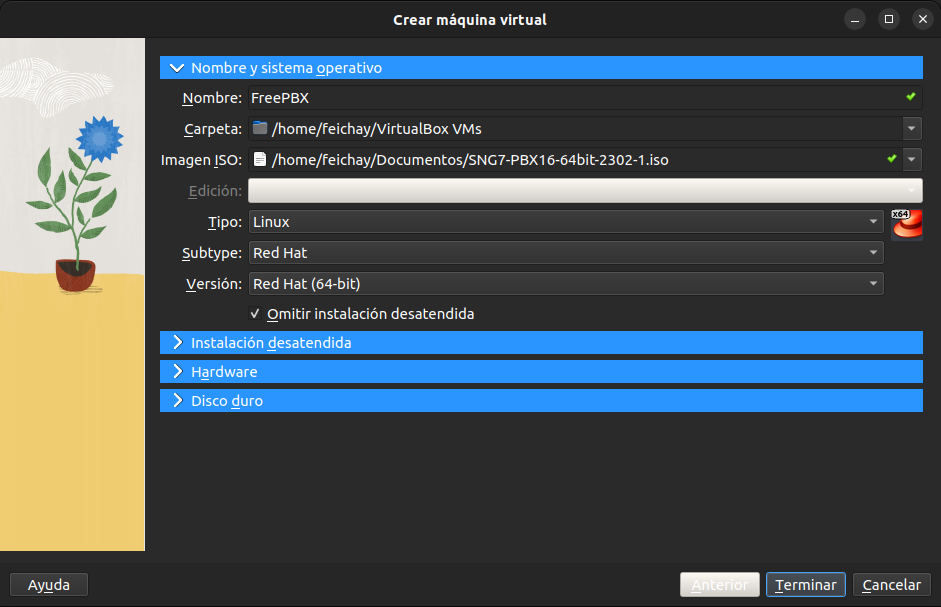
\includegraphics[width=\textwidth]{images/freepbx_virtualbox.png}
    \end{minipage}\hfill
    \begin{minipage}{0.49\textwidth}
        \centering
        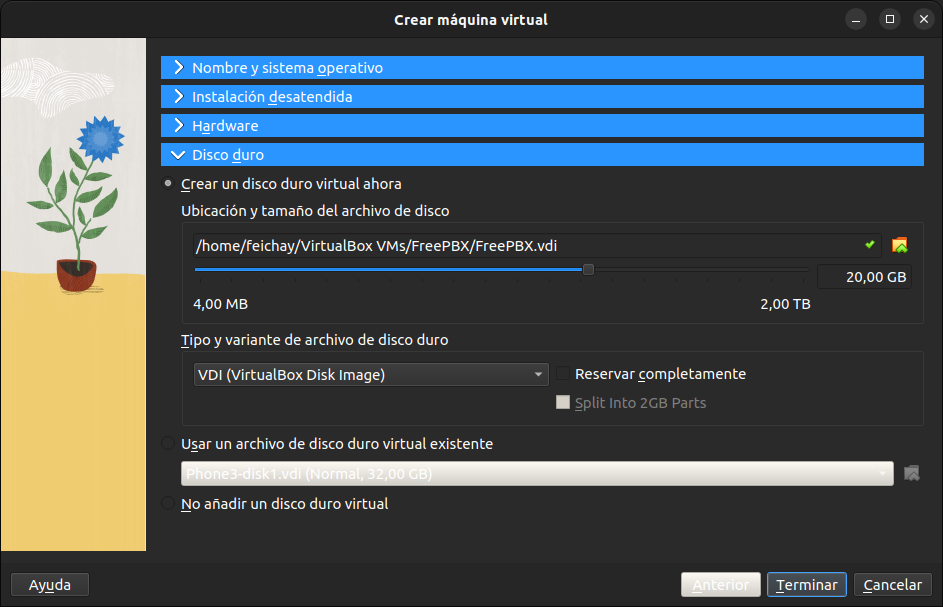
\includegraphics[width=\textwidth]{images/freepbx_virtualbox_2.png}
    \end{minipage}
		\caption{Configuración de la máquina virtual para FreePBX}
		\label{fig:freepbx_virtualbox}
\end{figure}

Una vez creada la máquina virtual, se debe configurara dos adaptadores de red. Pero antes, se debe crear un nuevo \texttt{Adaptador solo anfitrión} en VirtualBox, 
para ello ejecutamos el siguiente comando en la terminal:
\begin{lstlisting}[language=bash]
sudo VBoxManage hostonly create
\end{lstlisting}

\noindent
Esto creará un nuevo adaptador de red solo para el anfitrión. A continuación, se debe configurar los adaptadores de red para la máquina virtual FreePBX. Para ello, se debe seleccionar la máquina virtual creada y hacer clic en \texttt{Configuración}. En la sección \texttt{Red}, se debe seleccionar el adaptador \texttt{Adaptador 1} y configurarlo de la siguiente manera:
\begin{multicols}{2}
\begin{itemize}
		\item Habilitar adaptador de red: Sí
		\item Conectado a: Adaptador puente
		\item Nombre: <nombre de la interfaz de red del equipo>
		\item Promiscuo: Permitir todo
\end{itemize}

\columnbreak

\begin{itemize}
		\item Tipo de adaptador: Intel PRO/1000 MT Desktop (82540EM)
		\item Dirección MAC: Dejar en blanco
		\item Cable conectado: Sí
\end{itemize}
\end{multicols}

\noindent
A continuación, se debe configurar el \texttt{Adaptador 2} de la siguiente manera:
\begin{multicols}{2}
\begin{itemize}
		\item Habilitar adaptador de red: Sí
		\item Conectado a: Adaptador solo anfitrión
		\item Nombre: vboxnet0
		\item Promiscuo: Permitir todo
\end{itemize}

\columnbreak

\begin{itemize}
		\item Tipo de adaptador: Intel PRO/1000 MT Desktop (82540EM)
		\item Dirección MAC: Dejar en blanco
		\item Cable conectado: Sí
\end{itemize}
\end{multicols}

\noindent
Una vez creada los adaptadores de red, vamos a asignar una dirección IP al adaptador \texttt{Adaptador sólo anfitrión} creado anteriormente. Esto es para usar esta interfaz en la simulación de GNS3.
Para ello, en la parte superior izquierda de la ventana de VirtualBox, donde aparece \texttt{Herramientas} le damos al boton de propiedades y seleccionamos la pestaña \texttt{Red}. Y una vez dentro de
la pestaña, vemos la el adaptador creado anteriormente, \texttt{vboxnet0}, y abajo de este configuramos la dirección IP y la máscara de subred. En este caso, se ha configurado la dirección IP 
\texttt{192.168.1.135} y la máscara de subred \texttt{255.255.255.240}.

\begin{figure}[H]
	\centering
	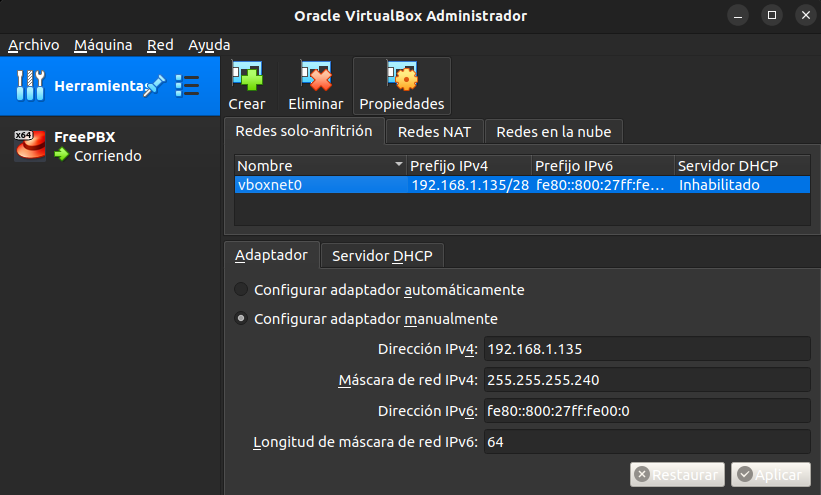
\includegraphics[width=0.8\textwidth]{images/freepbx_virtualbox_3.png}
	\caption{Configuración de la red en VirtualBox}
	\label{fig:freepbx_virtualbox_red}
\end{figure}

\noindent
Una vez configurada la red, se debe iniciar la máquina virtual y seguir las instrucciones de instalación de FreePBX. Selecionamos la primera opción y pulsamos \texttt{Enter} para iniciar la instalación. A continuación, saldrá \texttt{FreePBX Standard} y pulsamos \texttt{Enter} nuevamente para continuar con la instalación. Ya dentro de panel de configuración de FreePBX, hay que configurar el usuario y la contraseña para el usuario \texttt{root}. Para simplicidad, se ha configurado el usuario \texttt{root} con la contraseña \texttt{root}. Y esperamos a que se complete la instalación. Una vez completada la instalación, vamos a apagar la máquina virtual para eliminar el disco de instalación y arrancar desde el disco duro virtual.

\begin{figure}[H]
    \centering
    \begin{minipage}{0.49\textwidth}
        \centering
        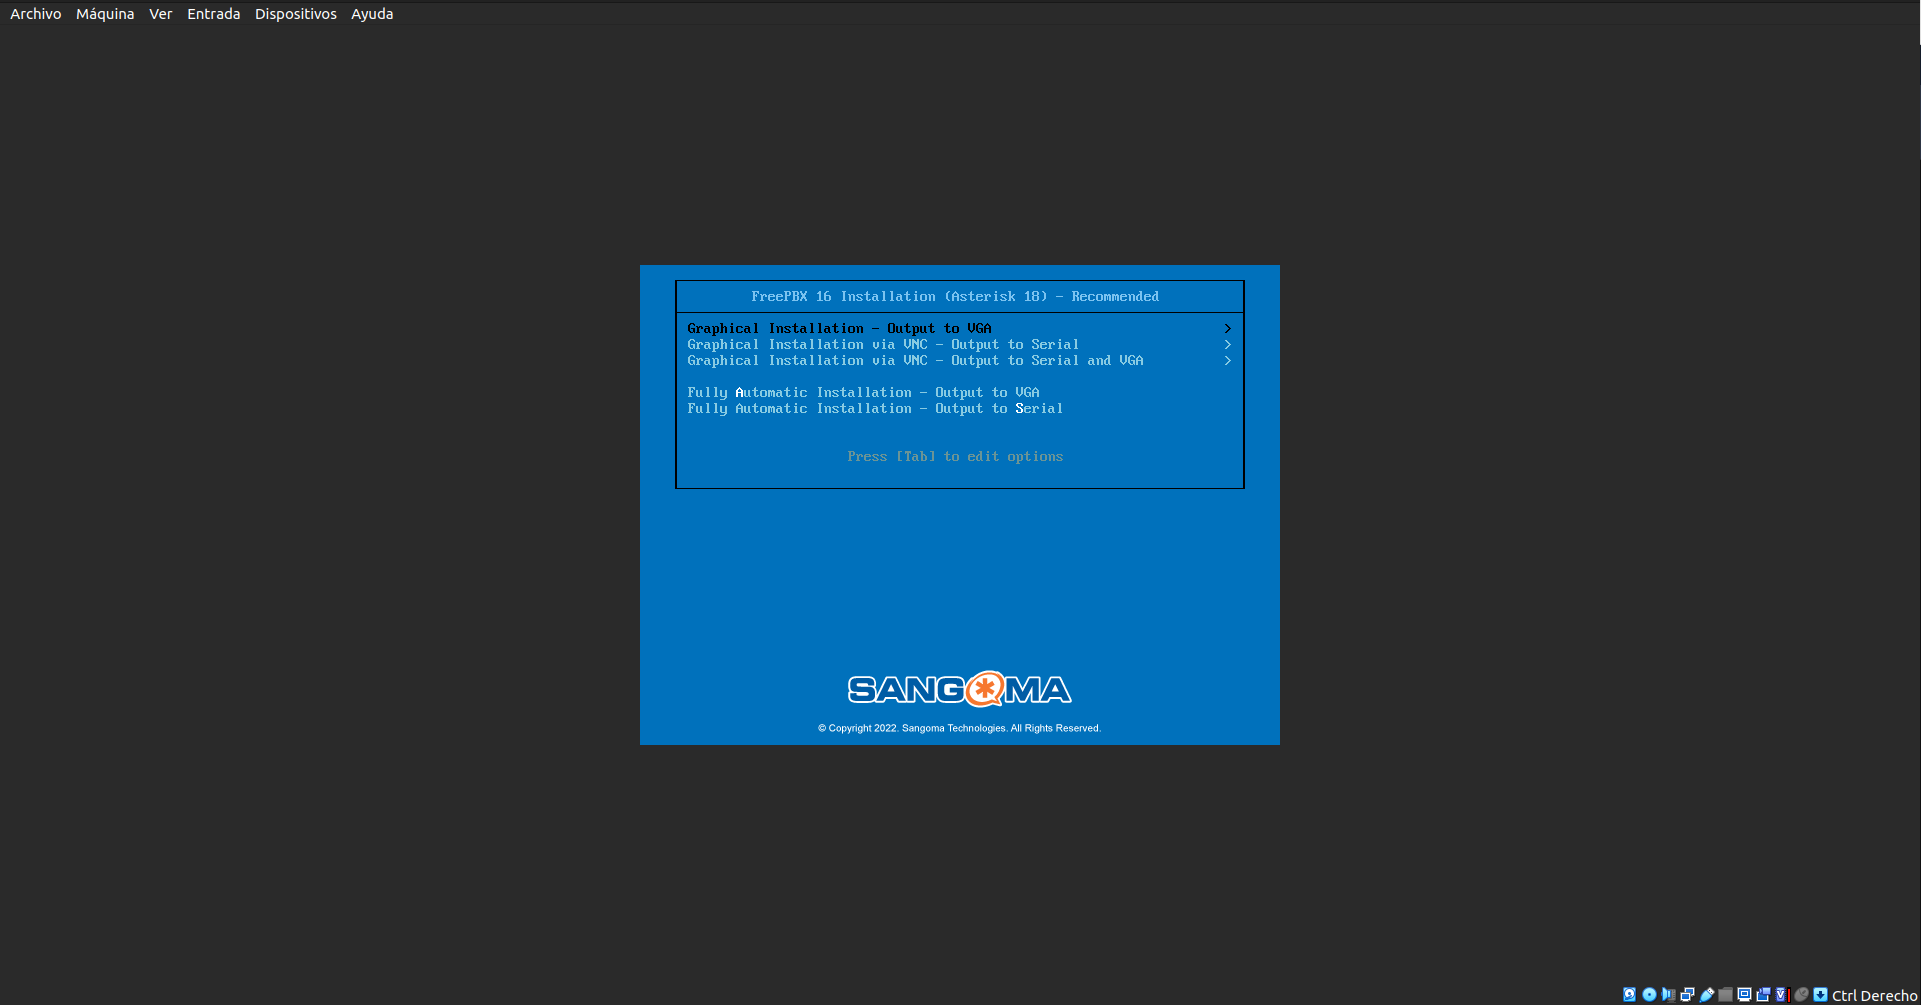
\includegraphics[width=\textwidth]{images/freepbx_installation_1.png}
    \end{minipage}\hfill
    \begin{minipage}{0.49\textwidth}
        \centering
        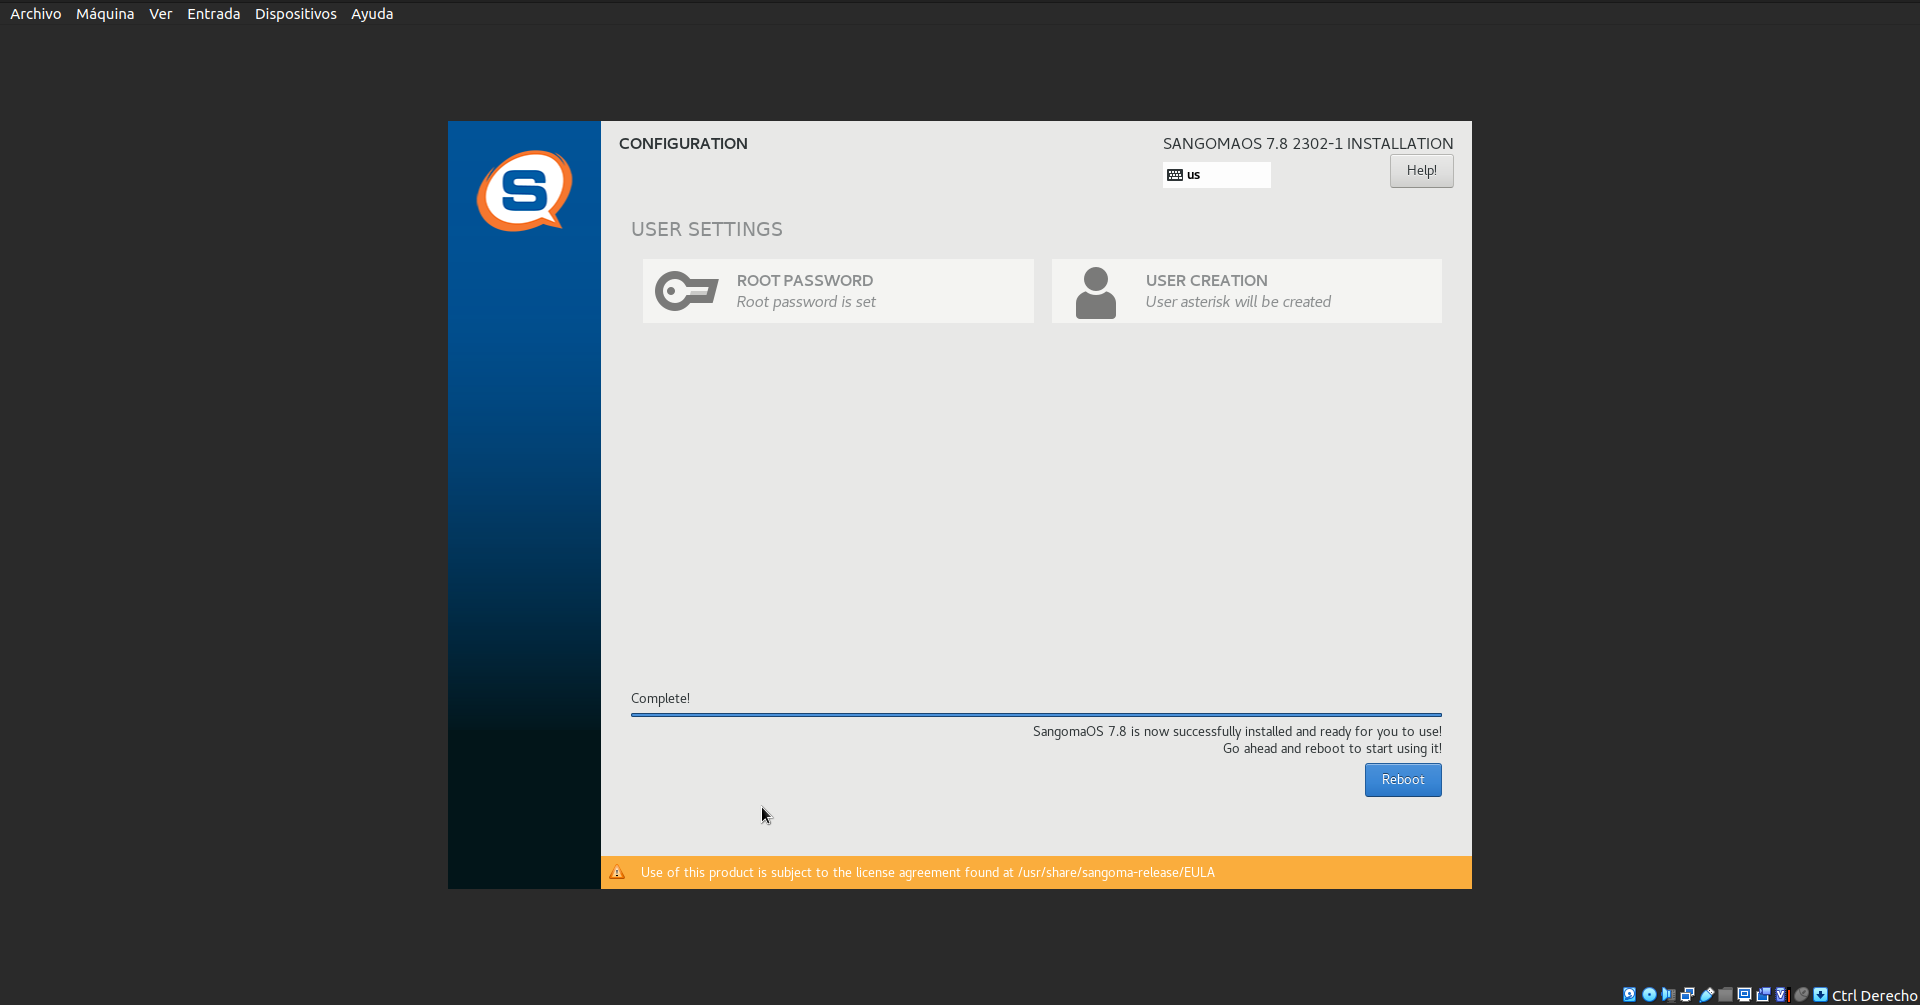
\includegraphics[width=\textwidth]{images/freepbx_installation_5.png}
    \end{minipage}
		\caption{Configuración de la máquina virtual para FreePBX}
		\label{fig:freepbx_installation_1}
\end{figure}

\noindent
Para ello, vamos a la configuración de la máquina virtual y en la sección \texttt{Almacenamiento} eliminamos el disco de instalación como se muestra en la figura~\ref{fig:freepbx_installation_6}.

\begin{figure}[H]
	\centering
	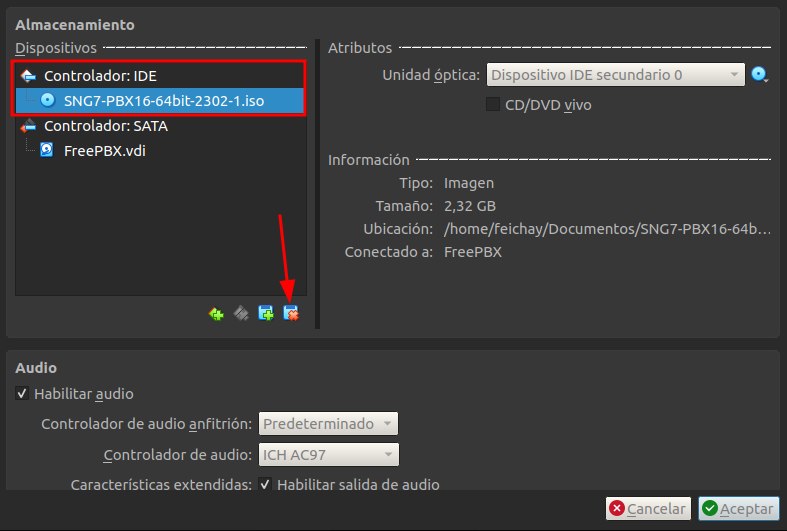
\includegraphics[width=0.8\textwidth]{images/freepbx_installation_6.png}
	\caption{Instalación de FreePBX}
	\label{fig:freepbx_installation_6}
\end{figure}

\noindent
Una vez eliminado el disco de instalación, iniciamos la máquina virtual y accedemos al panel de configuración de FreePBX con la dirección IP que se le ha asignado a la máquina virtual. En la figura~\ref{fig:freepbx_terminal.png} se muestra la dirección IP asignada a la máquina virtual, que en este caso es \texttt{192.168.1.31}.
\begin{figure}[H]
	\centering
	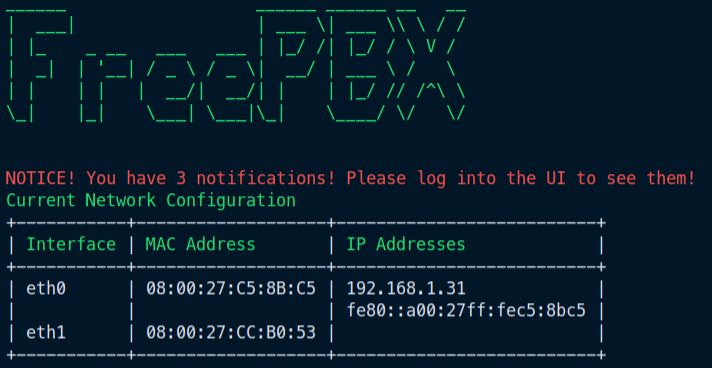
\includegraphics[width=0.8\textwidth]{images/freepbx_terminal.png}
	\caption{Panel de configuración de FreePBX}
	\label{fig:freepbx_terminal.png}
\end{figure}

\noindent
Para acceder al panel de configuración de FreePBX, se debe abrir un navegador web y acceder a la dirección IP asignada a la máquina virtual. En este caso, se ha accedido a la dirección 
\url{http://192.168.1.31/admin}. Una vez accedido al panel de configuración, se debe de crear el usuario administrador. Para simplificar, se ha creado el usuario \texttt{admin} con la contraseña \texttt{admin}.

\begin{figure}[H]
	\centering
	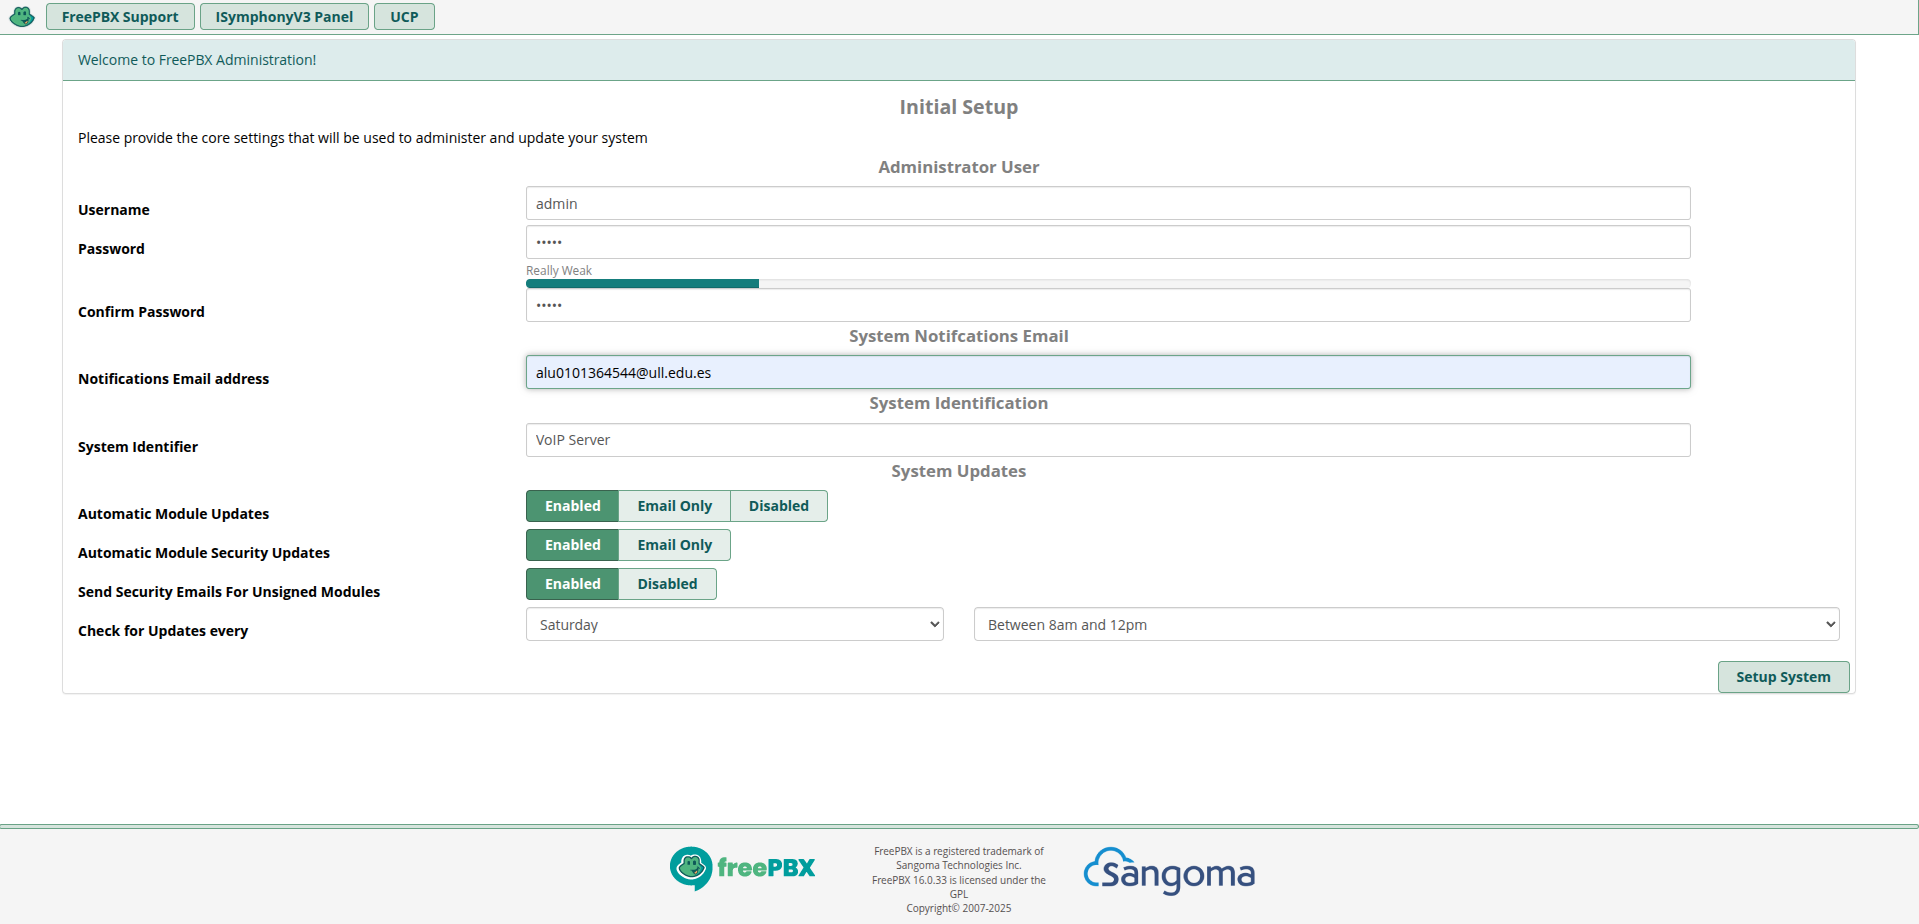
\includegraphics[width=0.8\textwidth]{images/freepbx_configuration_admin.png}
	\caption{Configuración de FreePBX}
	\label{fig:freepbx_configuration_admin}
\end{figure}

\subsection{Instalacion Softphone}
\label{Apendice1:instalacion_softphone}
Para la simulación de telefonos IPs en GNS3, se ha utilizado una máquina virtual ligera con el sistema operativo Windows 7 obtenido de un video tutorial de Youtube \cite{youtube_carlos_carrillo} de \texttt{Método para simular redes VoIP en GNS3}. Para instalar la máquina virtual, se ha descargado desde el enlace que proporciona el video tutorial y se ha importado a VirtualBox como un disco duro virtual en formato \texttt{.vdi} con el sistema operativo Windows 7 instalado y ya configurado.

\vspace{1em}
\noindent
Para importar la máquina virtual, se debe abrir VirtualBox y seleccionar \texttt{Nueva} para crear una nueva máquina virtual. Se debe poner un nombre, por ejemplo \texttt{Phone1}, seleccionar el tipo de sistema operativo, \texttt{Windows}, y la versión como \texttt{Windows 7 (64-bit)}. 

\begin{figure}[H]
	\centering
	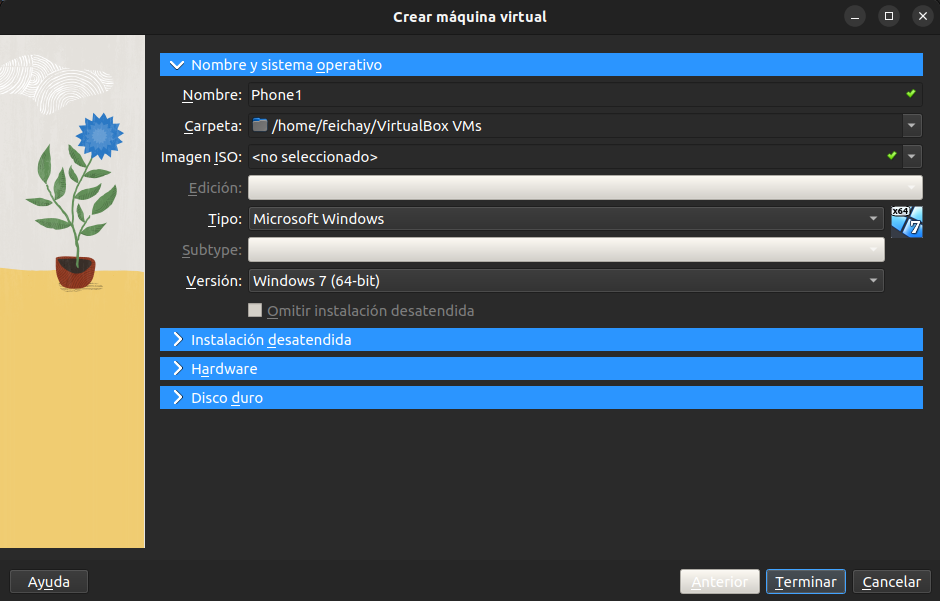
\includegraphics[width=0.8\textwidth]{images/softphone_1.png}
	\caption{Configuración de la máquina virtual para Softphone}
	\label{fig:softphone_1}
\end{figure}

\noindent
Luego, se debe asignar una cantidad de memoria RAM (256 MB es suficiente) y 1 CPU.

\begin{figure}[H]
	\centering
	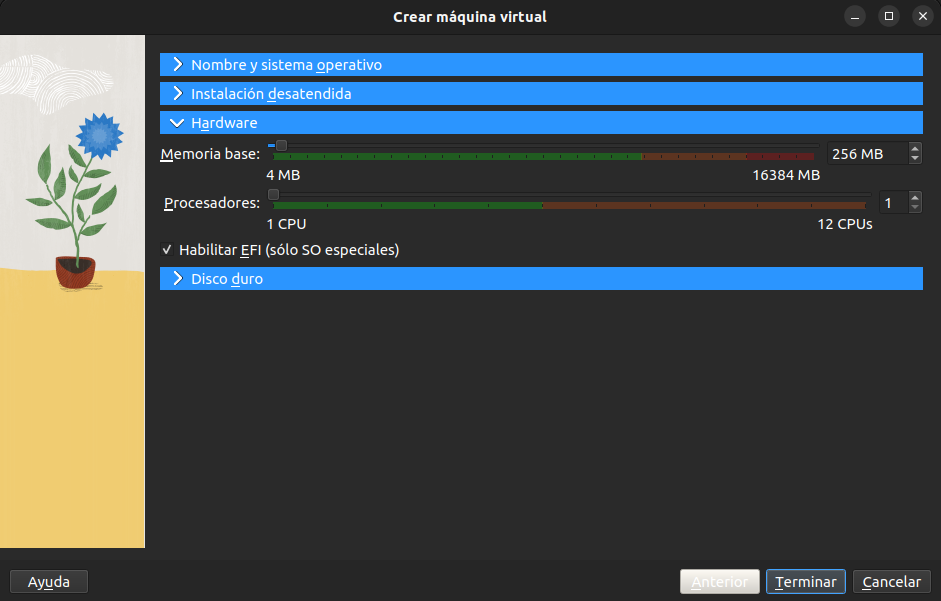
\includegraphics[width=0.8\textwidth]{images/softphone_2.png}
	\caption{Configuración de la máquina virtual para Softphone}
	\label{fig:softphone_2}
\end{figure}

\noindent
Por último, se debe seleccionar el disco duro virtual que se ha descargado previamente. Para ello, se debe seleccionar la opción \texttt{Usar un archivo de disco duro virtual existente} y seleccionar el archivo descargado.

\begin{figure}[H]
	\centering
	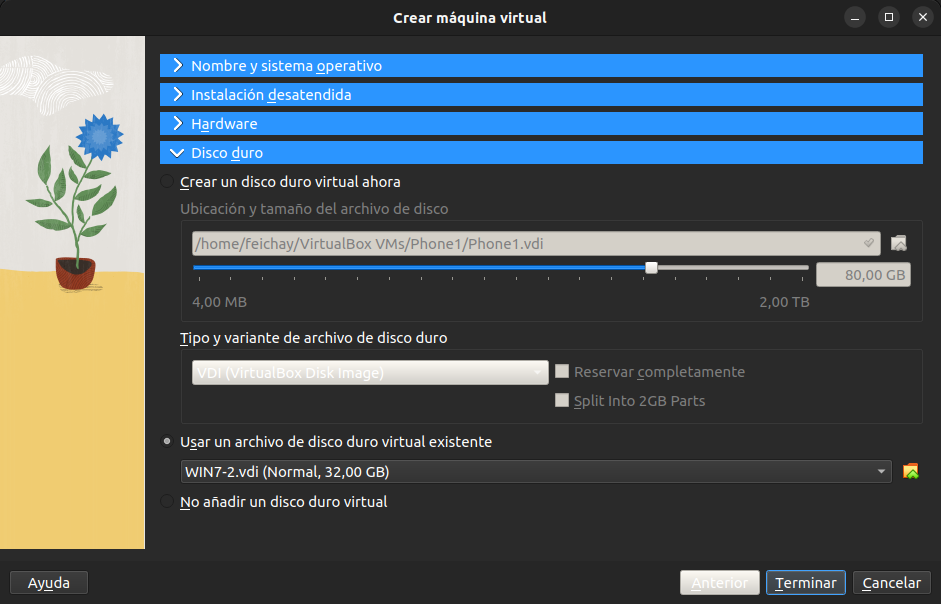
\includegraphics[width=0.8\textwidth]{images/softphone_3.png}
	\caption{Configuración de la máquina virtual para Softphone}
	\label{fig:softphone_3}
\end{figure}

\section{Instalación de Docker}
\label{Apendice1:instalacion_docker}
Para instalar Docker \cite{docker_ubuntu} y Docker Compose \cite{docker_compose_ubuntu} en Ubuntu, se deben seguir los siguientes pasos:

\subsection{Añadir el repositorio Docker}
Primero, instalar todas las dependencias necesarias usando el siguiente comando:
\begin{lstlisting}[language=bash]
sudo apt update
sudo apt install apt-transport-https ca-certificates curl software-properties-common -y
\end{lstlisting}

Después de instalar todas las dependencias, hay que descargar y añadir la clave GPG de Docker CE (Docker Community Edition) con el siguiente comando:
\begin{lstlisting}[language=bash]
curl -fsSL https://download.docker.com/linux/ubuntu/gpg | sudo apt-key add -
\end{lstlisting}

Ahora, añadimos el repositorio de Docker CE con el siguiente comando. Es importante notar que aunque la guía original mencione "focal" (para Ubuntu 20.04), para Ubuntu 22.04 (Jammy Jellyfish) se debería usar "jammy". Sin embargo, si se sigue una guía específica que indica "focal" y funciona, se puede mantener, pero es recomendable usar la versión correspondiente a la distribución:
\begin{lstlisting}[language=bash]
sudo add-apt-repository "deb [arch=amd64] https://download.docker.com/linux/ubuntu $(lsb_release -cs) stable"
\end{lstlisting}
O, si se desea usar "focal" explícitamente:
\begin{lstlisting}[language=bash]
sudo add-apt-repository "deb [arch=amd64] https://download.docker.com/linux/ubuntu focal stable"
\end{lstlisting}

Por último, verificar que se ha añadido el repositorio con el siguiente comando:
\begin{lstlisting}[language=bash]
apt-cache policy docker-ce
\end{lstlisting}

\subsection{Instalar Docker y Docker Compose}
Ahora, hay que instalar los paquetes de Docker usando el siguiente comando:
\begin{lstlisting}[language=bash]
sudo apt update
sudo apt install docker-ce -y
\end{lstlisting}

Una vez está Docker instalado, hay que verificar que Docker está corriendo correctamente:
\begin{lstlisting}[language=bash]
sudo systemctl status docker
\end{lstlisting}

Después, hay que instalar Docker Compose. La forma de instalar Docker Compose puede variar. Una forma común es descargarlo directamente desde GitHub. Sin embargo, si está disponible en los repositorios (como `docker-compose-plugin` o `docker-compose` v2), esa sería la forma preferida. La instrucción `apt install docker-compose -y` instalará la versión disponible en los repositorios de Ubuntu, que podría ser la v1. Para la v2, que se integra como un plugin de Docker CLI, los pasos serían diferentes.
\begin{lstlisting}[language=bash]
sudo apt install docker-compose -y
\end{lstlisting}
Para verificar la instalación de Docker Compose:
\begin{lstlisting}[language=bash]
docker-compose --version
\end{lstlisting}

	\chapter{\LARGE Configuración de los servicios y dispositivos}
	\label{appendix:2}
	\section{Configuración de los routers de la red de ISP}
Aquí se detalla la configuración de los routers utilizados en la simulación de la red de ISP, incluyendo los routers PE (Provider Edge), P (Provider) y CE (Customer Edge). 
\subsection{Configuración de los routers PE}
\label{Apendice2:configuracion_routers_pe}

\subsubsection*{Router PE1}
\begin{lstlisting}[language=RouterOS]
/system identity set name=PE1
/interface bridge add name=lo0
/ip address add address=1.1.1.11/32 interface=lo0 network=1.1.1.11
/ip address add address=10.0.0.1/30 interface=ether1 network=10.0.0.0
/ip address add address=172.16.0.1/30 interface=ether2 network=172.16.0.0
/ip address add address=10.0.0.13/30 interface=ether3 network=10.0.0.12

/routing ospf instance add name=backbone router-id=1.1.1.11
/routing ospf area add name=backbone area-id=0.0.0.0 inst=backbone
/routing ospf interface-template add interface=lo0 network=1.1.1.11/32 area=backbone
/routing ospf interface-template add interface=ether1 network=10.0.0.1/30 area=backbone

/mpls ldp add afi=ip lsr-id=1.1.1.11 transport-addresses=1.1.1.11
/mpls ldp interface add interface=lo0
/mpls ldp interface add interface=ether1
/mpls settings set dynamic-label-range=10000-11999

/routing bgp template set default address-families=ip,vpnv4 as=65000 router-id=1.1.1.11
/routing bgp connection
add connect=yes disabled=no listen=yes local.address=1.1.1.11 .role=ibgp \
    name=toPE2 remote.address=1.1.1.12 .as=65000 templates=default
/routing bgp connection
add connect=yes disabled=no listen=yes local.address=1.1.1.11 .role=ibgp \
    name=toPE3 remote.address=1.1.1.13 .as=65000 templates=default
/routing bgp connection
add connect=yes disabled=no listen=yes local.address=1.1.1.11 .role=ibgp \
    name=toPE4 remote.address=1.1.1.14 .as=65000 templates=default

/ip vrf add name=CE1 interfaces=ether2 

/routing bgp vpn
add export.redistribute=connected,static,bgp .route-targets=65000:100 \
    import.route-targets=65000:100 label-allocation-policy=per-vrf name=\
    bgp-mpls-vpn-1 route-distinguisher=65000:100 vrf=CE1

/routing bgp connection
add as=65000 connect=yes disabled=yes listen=yes local.address=172.16.0.1 \
    .role=ebgp name=toCE1 output.default-originate=always remote.address=\
    172.16.0.2 .as=65500 router-id=1.1.1.11 routing-table=CE1 vrf=CE1

/routing bgp connection add as=65000 connect=yes disabled=yes listen=yes local.address=172.16.0.1 .role=ebgp name=toCE1 output.default-originate=always remote.address=172.16.0.2 .as=65500 router-id=1.1.1.11 routing-table=CE1 vrf=CE1

/ip firewall mangle
add action=mark-routing chain=prerouting dst-address=!192.168.0.0/16 \
    in-interface=ether2 new-routing-mark=main passthrough=yes
/ip route add gateway=172.16.0.2@CE1 routing-table=CE1
/ip route add gateway=10.0.0.14
/ip route add dst-address=172.16.0.0/30 gateway=CE1@CE1 routing-table=main
\end{lstlisting}

\subsubsection*{Router PE2}
\begin{lstlisting}[language=RouterOS]
/system identity set name=PE2
/interface bridge add name=lo0
/ip address add address=1.1.1.12/32 interface=lo0
/ip address add address=172.16.0.5/30 interface=ether1
/ip address add address=10.0.0.5/30 interface=ether2

/routing ospf instance add name=backbone router-id=1.1.1.12
/routing ospf area add name=backbone area-id=0.0.0.0 inst=backbone
/routing ospf interface-template add interface=lo0 network=1.1.1.12/32 area=backbone
/routing ospf interface-template add interface=ether2 network=10.0.0.5/30 area=backbone

/mpls ldp add afi=ip lsr-id=1.1.1.12 transport-addresses=1.1.1.12
/mpls ldp interface add interface=ether2
/mpls settings set dynamic-label-range=12000-13999

/routing bgp template set default address-families=ip,vpnv4 as=65000 router-id=1.1.1.12
/routing bgp connection add name=toPE1 template=default local.address=1.1.1.12 local.role=ibgp remote.address=1.1.1.11 remote.as=65000 connect=yes listen=yes
/routing bgp connection add name=toPE3 template=default local.address=1.1.1.12 local.role=ibgp remote.address=1.1.1.13 remote.as=65000 connect=yes listen=yes
/routing bgp connection add name=toPE4 template=default local.address=1.1.1.12 local.role=ibgp remote.address=1.1.1.14 remote.as=65000 connect=yes listen=yes

/ip vrf add name=CE2 interfaces=ether1 

/routing bgp vpn add route-distinguisher=65000:100 import.route-targets=65000:100 vrf=CE2 label-allocation-policy=per-vrf export.route-targets=65000:100 .redistribute=connected,static,bgp

/routing bgp connection add name=toCE2 router-id=1.1.1.12 as=65000 local.address=172.16.0.5 .role=ebgp remote.address=172.16.0.6 .as=65500 routing-table=CE2 vrf=CE2 connect=yes listen=yes output.default-originate=always
\end{lstlisting}

\subsubsection*{Router PE3}
\begin{lstlisting}[language=RouterOS]
/system identity set name=PE3
/interface bridge add name=lo0
/ip address add address=1.1.1.13/32 interface=lo0
/ip address add address=10.0.0.9/30 interface=ether1
/ip address add address=172.16.0.9/30 interface=ether2

/routing ospf instance add name=backbone router-id=1.1.1.13
/routing ospf area add name=backbone area-id=0.0.0.0 inst=backbone
/routing ospf interface-template add interface=lo0 network=1.1.1.13/32 area=backbone
/routing ospf interface-template add interface=ether1 network=10.0.0.9/30 area=backbone

/mpls ldp add afi=ip lsr-id=1.1.1.13 transport-addresses=1.1.1.13
/mpls ldp interface add interface=ether1
/mpls settings set dynamic-label-range=14000-15999

/routing bgp template set default address-families=ip,vpnv4 as=65000 router-id=1.1.1.13
/routing bgp connection add name=toPE1 template=default local.address=1.1.1.13 local.role=ibgp remote.address=1.1.1.11 remote.as=65000 connect=yes listen=yes
/routing bgp connection add name=toPE2 template=default local.address=1.1.1.13 local.role=ibgp remote.address=1.1.1.12 remote.as=65000 connect=yes listen=yes
/routing bgp connection add name=toPE4 template=default local.address=1.1.1.13 local.role=ibgp remote.address=1.1.1.14 remote.as=65000 connect=yes listen=yes

/ip vrf add name=CE3 interfaces=ether2 

/routing bgp vpn add route-distinguisher=65000:100 import.route-targets=65000:100 vrf=CE3 label-allocation-policy=per-vrf export.route-targets=65000:100 .redistribute=connected,static,bgp

/routing bgp connection add name=toCE3 router-id=1.1.1.13 as=65000 local.address=172.16.0.9 .role=ebgp remote.address=172.16.0.10 .as=65500 routing-table=CE3 vrf=CE3 connect=yes listen=yes output.default-originate=always
\end{lstlisting}

\subsection{Configuración de los routers P}
\label{Apendice2:configuracion_routers_p}

\subsubsection*{Router P1}
\begin{lstlisting}[language=RouterOS]
/system identity set name=P1
/interface bridge add name=lo0
/ip address add address=1.1.1.1/32 interface=lo0
/ip address add address=10.0.0.18/30 interface=ether1
/ip address add address=10.0.0.26/30 interface=ether2
/ip address add address=10.0.0.6/30 interface=ether3
/ip address add address=10.0.0.10/30 interface=ether4

/routing ospf instance add name=backbone router-id=1.1.1.1
/routing ospf area add name=backbone area-id=0.0.0.0 inst=backbone
/routing ospf interface-template add interface=lo0 network=1.1.1.1/32 area=backbone
/routing ospf interface-template add interface=ether1 network=10.0.0.18/30 area=backbone
/routing ospf interface-template add interface=ether2 network=10.0.0.26/30 area=backbone
/routing ospf interface-template add interface=ether3 network=10.0.0.6/30 area=backbone
/routing ospf interface-template add interface=ether4 network=10.0.0.10/30 area=backbone

/mpls ldp add afi=ip lsr-id=1.1.1.1 transport-addresses=1.1.1.1
/mpls ldp interface add interface=lo0
/mpls ldp interface add interface=ether1
/mpls ldp interface add interface=ether2
/mpls ldp interface add interface=ether3
/mpls ldp interface add interface=ether4
/mpls settings set dynamic-label-range=20000-21999
\end{lstlisting}

\subsubsection*{Router P2}
\begin{lstlisting}[language=RouterOS]
/system identity set name=P3
/interface bridge add name=lo0
/ip address add address=1.1.1.3/32 interface=lo0
/ip address add address=10.0.0.21/30 interface=ether1
/ip address add address=10.0.0.17/30 interface=ether2
/ip address add address=10.0.0.2/30 interface=ether3
/ip address add address=10.0.0.14/30 interface=ether4

/routing ospf instance add name=backbone router-id=1.1.1.3
/routing ospf area add name=backbone area-id=0.0.0.0 inst=backbone
/routing ospf interface-template add interface=lo0 network=1.1.1.3/32 area=backbone
/routing ospf interface-template add interface=ether1 network=10.0.0.21/30 area=backbone
/routing ospf interface-template add interface=ether2 network=10.0.0.17/30 area=backbone
/routing ospf interface-template add interface=ether3 network=10.0.0.2/30 area=backbone
/routing ospf interface-template add interface=ether4 network=10.0.0.14/30 area=backbone

/mpls ldp add afi=ip lsr-id=1.1.1.3 transport-addresses=1.1.1.3
/mpls ldp interface add interface=lo0
/mpls ldp interface add interface=ether1
/mpls ldp interface add interface=ether2
/mpls ldp interface add interface=ether3
/mpls ldp interface add interface=ether4
/mpls settings set dynamic-label-range=24000-25999
\end{lstlisting}

\subsubsection*{Router P3}
\begin{lstlisting}[language=RouterOS]
/system identity set name=P3
/interface bridge add name=lo0
/ip address add address=1.1.1.3/32 interface=lo0
/ip address add address=10.0.0.21/30 interface=ether1
/ip address add address=10.0.0.17/30 interface=ether2
/ip address add address=10.0.0.2/30 interface=ether3
/ip address add address=10.0.0.14/30 interface=ether4

/routing ospf instance add name=backbone router-id=1.1.1.3
/routing ospf area add name=backbone area-id=0.0.0.0 inst=backbone
/routing ospf interface-template add interface=lo0 network=1.1.1.3/32 area=backbone
/routing ospf interface-template add interface=ether1 network=10.0.0.21/30 area=backbone
/routing ospf interface-template add interface=ether2 network=10.0.0.17/30 area=backbone
/routing ospf interface-template add interface=ether3 network=10.0.0.2/30 area=backbone
/routing ospf interface-template add interface=ether4 network=10.0.0.14/30 area=backbone

/mpls ldp add afi=ip lsr-id=1.1.1.3 transport-addresses=1.1.1.3
/mpls ldp interface add interface=lo0
/mpls ldp interface add interface=ether1
/mpls ldp interface add interface=ether2
/mpls ldp interface add interface=ether3
/mpls ldp interface add interface=ether4
/mpls settings set dynamic-label-range=24000-25999
\end{lstlisting}

\subsection{Configuración de los routers CE}
\label{Apendice2:configuracion_routers_ce}

\subsubsection*{Router CE1}
\begin{lstlisting}[language=RouterOS]
/system identity set name=CE1
/interface bridge add name=lo0
/ip address add address=1.1.1.21/32 interface=lo0 network=1.1.1.21
/ip address add address=192.168.1.1/24 interface=ether1 network=192.168.1.0
/ip address add address=172.16.0.2/30 interface=ether2 network= 172.16.0.0

/ip firewall address-list add address=192.168.1.0/24 list=BGP_OUT
/ip firewall nat add action=masquerade chain=srcnat dst-address=!192.168.0.0/16 out-interface=ether2

/ip route add gateway=172.16.0.1

/routing bgp connection
add as=65500 connect=yes listen=yes local.address=172.16.0.2 .role=ebgp name=\
    toPE1 output.network=BGP_OUT remote.address=172.16.0.1 .as=65000 router-id=\
    1.1.1.21
\end{lstlisting}

\subsubsection*{Router CE2}
\begin{lstlisting}[language=RouterOS]
/system identity set name=CE3
/interface bridge add name=lo0
/ip address add address=1.1.1.23/32 interface=lo0
/ip address add address=172.16.0.10/30 interface=ether1
/ip address add address=192.168.3.1/24 interface=ether2

/ip firewall address-list add address=192.168.3.0/24 list=BGP_OUT
/routing bgp connection add name=toPE3 as=65500 router-id=1.1.1.23 local.address=172.16.0.10 .role=ebgp remote.address=172.16.0.9 remote.as=65000 output.network=BGP_OUT connect=yes listen=yes
\end{lstlisting}

\subsubsection*{Router CE3}
\begin{lstlisting}[language=RouterOS]
/system identity set name=CE3
/interface bridge add name=lo0
/ip address add address=1.1.1.23/32 interface=lo0
/ip address add address=172.16.0.10/30 interface=ether1
/ip address add address=192.168.3.1/24 interface=ether2

/ip firewall address-list add address=192.168.3.0/24 list=BGP_OUT
/routing bgp connection add name=toPE3 as=65500 router-id=1.1.1.23 local.address=172.16.0.10 .role=ebgp remote.address=172.16.0.9 remote.as=65000 output.network=BGP_OUT connect=yes listen=yes
\end{lstlisting}

\section{Configuracion de la Oficina Central}
\subsection{Configuración router CE1}
\label{Apendice2:configuracion_ce1}
Se presenta a continuación la configuración del router CE1, que incluye la creación de VLANs, la asignación de direcciones IP y la configuración de DHCP Relay para reenviar solicitudes al servidor DHCP ubicado en la DMZ.
\begin{lstlisting}[language=RouterOS]
# ------------------------------------------------------------
# Identidad
/system identity set name=CE1

# ------------------------------------------------------------
# Habilitar todas las interfaces físicas
/interface ethernet enable [find]

# ------------------------------------------------------------
# Crear Bonding con LACP (802.3ad) (EtherChannel)
/interface bonding add name=bond1 mode=802.3ad slaves=ether1,ether2 transmit-hash-policy=layer-2-and-3

# ------------------------------------------------------------
# VLANs sobre el bonding
/interface vlan add name=vlan10-datos vlan-id=10 interface=bond1 mtu=1480
/interface vlan add name=vlan20-voz   vlan-id=20 interface=bond1 mtu=1480
/interface vlan add name=vlan30-dmz   vlan-id=30 interface=bond1 mtu=1480

# ------------------------------------------------------------
# Asignar direcciones IPv6 a cada VLAN
/ipv6 address add address=2001:db8:1234:0100::1/64 interface=vlan10-datos
/ipv6 address add address=2001:db8:1234:0101::1/64 interface=vlan20-voz
/ipv6 address add address=2001:db8:1234:0102::1/64 interface=vlan30-dmz

# ------------------------------------------------------------
# Configuración VRRP en las VLANs
/interface vrrp add name=vrrp-datos interface=vlan10-datos vrid=10 priority=150 version=3 v3-protocol=ipv6 mtu=1480
/interface vrrp add name=vrrp-voz   interface=vlan20-voz   vrid=20 priority=150 version=3 v3-protocol=ipv6 mtu=1480
/interface vrrp add name=vrrp-dmz   interface=vlan30-dmz   vrid=30 priority=150 version=3 v3-protocol=ipv6 mtu=1480

# Direcciones virtuales VRRP
/ipv6 address add address=2001:db8:1234:0100::2/64 interface=vrrp-datos
/ipv6 address add address=2001:db8:1234:0101::2/64 interface=vrrp-voz
/ipv6 address add address=2001:db8:1234:0102::2/64 interface=vrrp-dmz

# ------------------------------------------------------------
# Conexion directa con CE1_Backup (enlace de sincronización)
/interface ethernet enable ether3
/ipv6 address add address=2001:db8:1234:0103::1/64 interface=ether3

# ------------------------------------------------------------
# DHCPv6 relay en VLANs
/ipv6 dhcp-relay add name=relay-datos interface=vlan10-datos dhcp-server=2001:db8:1234:0102::132 link-address=2001:db8:1234:0100::1 disabled=no
/ipv6 dhcp-relay add name=relay-voz   interface=vlan20-voz   dhcp-server=2001:db8:1234:0102::132 link-address=2001:db8:1234:0101::1 disabled=no

# ------------------------------------------------------------
# Neighbor Discovery (RA, DNS)
/ipv6 nd add interface=vlan10-datos advertise-dns=yes managed-address-configuration=yes other-configuration=yes ra-lifetime=1800 ra-preference=low dns=2001:db8:1234:0102::133,2001:db8:1234:0102::134
/ipv6 nd add interface=vlan20-voz   advertise-dns=yes managed-address-configuration=yes other-configuration=yes ra-lifetime=1800 ra-preference=low dns=2001:db8:1234:0102::133,2001:db8:1234:0102::134
/ipv6 nd add interface=vlan30-dmz   advertise-dns=yes dns=2001:db8:1234:0102::133,2001:db8:1234:0102::134

# ------------------------------------------------------------
# Firewall básico IPv6
/ipv6 firewall filter add chain=forward action=accept protocol=udp dst-port=53 comment="Permitir tráfico DNS"
/ipv6 firewall filter add chain=forward action=accept protocol=tcp dst-port=53 comment="Permitir tráfico DNS"
/ipv6 firewall filter add chain=forward action=accept protocol=udp dst-port=547 comment="Permitir tráfico DHCPv6"
/ipv6 firewall filter add chain=forward action=accept comment="Permitir comunicación entre VLANs"
/ipv6 firewall filter add chain=forward action=accept protocol=icmpv6 comment="Permitir tráfico ICMPv6 entre VLANs y servidor DNS"
/ipv6 firewall filter add chain=forward action=accept src-address=2001:db8:1234:0100::/64 dst-address=2001:db8:1234:0102::/64 comment="Datos → DMZ"
/ipv6 firewall filter add chain=forward action=accept src-address=2001:db8:1234:0101::/64 dst-address=2001:db8:1234:0102::/64 comment="Voz → DMZ"
/ipv6 firewall filter add chain=forward action=accept src-address=2001:db8:1234:0102::/64 dst-address=2001:db8:1234:0100::/64 comment="DMZ → Datos"
/ipv6 firewall filter add chain=forward action=accept src-address=2001:db8:1234:0102::/64 dst-address=2001:db8:1234:0101::/64 comment="DMZ → Voz"

# ------------------------------------------------------------
# Activar fast-path (si aplica)
/ip settings set allow-fast-path=yes

# ------------------------------------------------------------
# Guardar configuración
/system backup save name=CE1
\end{lstlisting}

\subsection{Configuración del router CE1\_backup ARREGLAR}
\label{Apendice2:configuracion_ce1_backup}
\begin{lstlisting}[language=RouterOS]
# ------------------------------------------------------------
# Identidad
/system identity set name=CE1-Backup

# ------------------------------------------------------------
# Habilitar todas las interfaces físicas
/interface ethernet enable [find]

# ------------------------------------------------------------
# Crear Bonding con LACP (802.3ad) (EtherChannel)
/interface bonding add name=bond1 mode=802.3ad slaves=ether1,ether2 transmit-hash-policy=layer-2-and-3

# ------------------------------------------------------------
# VLANs sobre el bonding
/interface vlan add name=vlan10-datos vlan-id=10 interface=bond1 mtu=1480
/interface vlan add name=vlan20-voz   vlan-id=20 interface=bond1 mtu=1480
/interface vlan add name=vlan30-dmz   vlan-id=30 interface=bond1 mtu=1480

# ------------------------------------------------------------
# Asignar direcciones IPv6 a cada VLAN
/ipv6 address add address=2001:db8:1234:0100::1/64 interface=vlan10-datos
/ipv6 address add address=2001:db8:1234:0101::1/64 interface=vlan20-voz
/ipv6 address add address=2001:db8:1234:0102::1/64 interface=vlan30-dmz

# ------------------------------------------------------------
# Configuración VRRP en las VLANs
/interface vrrp add name=vrrp-datos interface=vlan10-datos vrid=10 priority=100 version=3 v3-protocol=ipv6 mtu=1480
/interface vrrp add name=vrrp-voz   interface=vlan20-voz   vrid=20 priority=100 version=3 v3-protocol=ipv6 mtu=1480 
/interface vrrp add name=vrrp-dmz   interface=vlan30-dmz   vrid=30 priority=100 version=3 v3-protocol=ipv6 mtu=1480

# Direcciones virtuales VRRP
/ipv6 address add address=2001:db8:1234:0100::2/64 interface=vrrp-datos
/ipv6 address add address=2001:db8:1234:0101::2/64 interface=vrrp-voz
/ipv6 address add address=2001:db8:1234:0102::2/64 interface=vrrp-dmz

# ------------------------------------------------------------
# Conexion directa con CE (enlace de sincronización)
/interface ethernet enable ether3
/ipv6 address add address=2001:db8:1234:0103::2/64 interface=ether3

# ------------------------------------------------------------
# DHCPv6 relay en VLANs
/ipv6 dhcp-relay add name=relay-datos interface=vlan10-datos dhcp-server=2001:db8:1234:0102::132 link-address=2001:db8:1234:0100::1 disabled=no
/ipv6 dhcp-relay add name=relay-voz   interface=vlan20-voz   dhcp-server=2001:db8:1234:0102::132 link-address=2001:db8:1234:0101::1 disabled=no

# ------------------------------------------------------------
# Neighbor Discovery (RA, DNS)
/ipv6 nd add interface=vlan10-datos advertise-dns=yes managed-address-configuration=yes other-configuration=yes ra-lifetime=1800 ra-preference=low dns=2001:db8:1234:0102::133,2001:db8:1234:0102::134
/ipv6 nd add interface=vlan20-voz   advertise-dns=yes managed-address-configuration=yes other-configuration=yes ra-lifetime=1800 ra-preference=low dns=2001:db8:1234:0102::133,2001:db8:1234:0102::134
/ipv6 nd add interface=vlan30-dmz   advertise-dns=yes dns=2001:db8:1234:0102::133,2001:db8:1234:0102::134

# ------------------------------------------------------------
# Firewall básico IPv6
/ipv6 firewall filter add chain=forward action=accept protocol=udp dst-port=53 comment="Permitir tráfico DNS"
/ipv6 firewall filter add chain=forward action=accept protocol=tcp dst-port=53 comment="Permitir tráfico DNS"
/ipv6 firewall filter add chain=forward action=accept protocol=udp dst-port=547 comment="Permitir tráfico DHCPv6"
/ipv6 firewall filter add chain=forward action=accept comment="Permitir comunicación entre VLANs"
/ipv6 firewall filter add chain=forward action=accept protocol=icmpv6 comment="Permitir tráfico ICMPv6 entre VLANs y servidor DNS"
/ipv6 firewall filter add chain=forward action=accept src-address=2001:db8:1234:0100::/64 dst-address=2001:db8:1234:0102::/64 comment="Datos → DMZ"
/ipv6 firewall filter add chain=forward action=accept src-address=2001:db8:1234:0101::/64 dst-address=2001:db8:1234:0102::/64 comment="Voz → DMZ"
/ipv6 firewall filter add chain=forward action=accept src-address=2001:db8:1234:0102::/64 dst-address=2001:db8:1234:0100::/64 comment="DMZ → Datos"
/ipv6 firewall filter add chain=forward action=accept src-address=2001:db8:1234:0102::/64 dst-address=2001:db8:1234:0101::/64 comment="DMZ → Voz"

# ------------------------------------------------------------
# Activar fast-path (si aplica)
/ip settings set allow-fast-path=yes

# ------------------------------------------------------------
# Guardar configuración
/system backup save name=CE1-Backup
\end{lstlisting}

\subsection{Docker Compose para los servicios de red}
\label{Apendice2:docker_compose}
\begin{lstlisting}[language=yaml]
  services:
  dns-primary-ipv6:
    build:
      context: ./dns-primary-ipv6
      dockerfile: Dockerfile
    image: dns-primary-ipv6:latest
    container_name: dns-primary-ipv6
    hostname: dns-primary-ipv6
    networks:
      services_net:
        ipv6_address: 2001:db8:1234:0102::133
    volumes:
      - ./dns-primary-ipv6/named.conf.options:/etc/bind/named.conf.options
      - ./dns-primary-ipv6/named.conf.local:/etc/bind/named.conf.local
      - ./dns-primary-ipv6/zones/:/etc/bind/zones/
    cap_add:
      - NET_ADMIN
    privileged: true
    restart: unless-stopped

  dns-secondary-ipv6:
    build:
      context: ./dns-secondary-ipv6
      dockerfile: Dockerfile
    image: dns-secondary-ipv6:latest
    container_name: dns-secondary-ipv6
    hostname: dns-secondary-ipv6
    networks:
      services_net:
        ipv6_address: 2001:db8:1234:0102::134
    volumes:
      - ./dns-secondary-ipv6/named.conf.options:/etc/bind/named.conf.options
      - ./dns-secondary-ipv6/named.conf.local:/etc/bind/named.conf.local
      - ./dns-secondary-ipv6/zones/:/etc/bind/zones/
    cap_add:
      - NET_ADMIN
    privileged: true
    restart: unless-stopped

  dhcp6-server:
    build:
      context: ./dhcp6-server
      dockerfile: Dockerfile
    image: dhcp6-server:latest
    container_name: dhcp6-server
    hostname: dhcp6-server
    networks:
      services_net:
        ipv6_address: 2001:db8:1234:0102::132
    volumes:
      - ./dhcp6-server/dhcpd6.conf:/etc/dhcp/dhcpd6.conf
      - ./dhcp6-server/isc-dhcp-server:/etc/default/isc-dhcp-server
    cap_add:
      - NET_ADMIN
    privileged: true
    restart: unless-stopped

networks:
  services_net:
    driver: bridge
    enable_ipv6: true
    ipam:
      driver: default
      config:
        - subnet: "2001:db8:1234:0102::/64"
\end{lstlisting}

\subsection{Servidor DHCP}
Aqui se presenta la configuración del servidor DHCP, tanto el Dockerfile como los archivos de configuración.

\newpage

\subsubsection{Dockerfile para el servidor DHCP}
\label{Apendice2:dockerfile_dhcp}
\begin{lstlisting}[language=Dockerfile]
FROM ubuntu:20.04

# Evitar prompts interactivos durante la instalación
ENV DEBIAN_FRONTEND=noninteractive

# Actualizar e instalar paquetes necesarios
RUN apt-get update && apt-get install -y \
    isc-dhcp-server \
    iputils-ping \
    net-tools \
    iproute2 \
    procps \
    && apt-get clean \
    && rm -rf /var/lib/apt/lists/*

# Crear directorio para logs y leases
RUN mkdir -p /var/log /var/lib/dhcp /var/run

# Crear archivo de leases inicial (requerido por dhcpd)
RUN touch /var/lib/dhcp/dhcpd6.leases

# Establecer permisos correctos
RUN chown -R dhcpd:dhcpd /var/lib/dhcp /var/log
RUN chmod 644 /var/lib/dhcp/dhcpd6.leases

# Copiar archivos de configuración del DHCP
COPY dhcpd6.conf /etc/dhcp/dhcpd6.conf
COPY isc-dhcp-server /etc/default/isc-dhcp-server

# Establecer permisos correctos para los archivos de configuración
RUN chmod 644 /etc/dhcp/dhcpd6.conf
RUN chmod 644 /etc/default/isc-dhcp-server

# Crear script de inicio
RUN echo '#!/bin/bash\n\
# Configurar IP estática dinámicamente\n\
ip -6 addr add 2001:db8:1234:0102::132/64 dev eth0\n\
ip -6 route add default via 2001:db8:1234:0102::1\n\
echo "nameserver 2001:db8:1234:0102::133" > /etc/resolv.conf\n\
echo "nameserver 2001:db8:1234:0102::134" >> /etc/resolv.conf\n\
# Iniciar servidor DHCP\n\
exec dhcpd -6 -cf /etc/dhcp/dhcpd6.conf -d eth0; exec bash' > /start.sh

RUN chmod +x /start.sh

# Crear usuario dhcpd si no existe
RUN useradd -r -s /bin/false dhcpd 2>/dev/null || true

# Exponer puerto DHCP
EXPOSE 547/udp

# Usar el script de inicio
CMD ["/start.sh"] 
\end{lstlisting}

\subsubsection{Archivo dhcpd6.conf}
\label{Apendice2:dhcpd6.conf}
\begin{lstlisting}[language=bash]
default-lease-time 600;
max-lease-time 7200;
authoritative;

option dhcp6.domain-search "cazg.es";
option dhcp6.name-servers 2001:db8:1234:0102::133, 2001:db8:1234:0102::134;

# VLAN Datos: 2001:db8:1234:0100::/64
subnet6 2001:db8:1234:0100::/64  {
    range6 2001:db8:1234:0100::2 2001:db8:1234:0100::ffff;
}

# VLAN Voz: 2001:db8:1234:0101::/64
subnet6 2001:db8:1234:0101::/64 {
    range6 2001:db8:1234:0101::2 2001:db8:1234:0101::ffff;
}

# VLAN DMZ: 2001:db8:1234:0102::/64
subnet6 2001:db8:1234:0102::/64 { }
\end{lstlisting}

\subsection{Servidor DNS Primario}
Aqui se presenta la configuración del servidor DNS primario, tanto el Dockerfile como los archivos de configuración.

\subsubsection{Dockerfile para el servidor DNS primario}
\label{Apendice2:dockerfile_dns_primario}
\begin{lstlisting}[language=Dockerfile]
FROM ubuntu:20.04

# Evitar prompts interactivos durante la instalación
ENV DEBIAN_FRONTEND=noninteractive

# Actualizar e instalar paquetes necesarios
RUN apt-get update && apt-get install -y \
    bind9 \
    bind9utils \
    bind9-doc \
    iputils-ping \
    net-tools \
    ifupdown \
    && apt-get clean \
    && rm -rf /var/lib/apt/lists/*

# Crear directorios necesarios
RUN mkdir -p /etc/bind/zones /var/cache/bind /var/lib/bind /var/log/named

# Copiar archivos de configuración DNS
COPY named.conf.options /etc/bind/
COPY named.conf.local /etc/bind/
COPY zones/ /etc/bind/zones/

# Establecer permisos correctos para bind
RUN chown -R bind:bind /etc/bind/zones /var/cache/bind /var/lib/bind /var/log/named
RUN chmod 755 /etc/bind/zones
RUN chmod 775 /var/cache/bind
RUN chmod 644 /etc/bind/named.conf.options /etc/bind/named.conf.local
RUN chmod 644 /etc/bind/zones/*

# Crear script de inicio
RUN echo '#!/bin/bash\n\
# Configurar IP estática dinámicamente\n\
ip addr add 192.168.1.133/28 dev eth0\n\
ip route add default via 192.168.1.131\n\
echo "nameserver 192.168.1.133" > /etc/resolv.conf\n\
echo "nameserver 192.168.1.134" >> /etc/resolv.conf\n\
# Iniciar servidor DNS\n\
exec named -g -c /etc/bind/named.conf -u bind; exec bash' > /start.sh

RUN chmod +x /start.sh

# Exponer puertos DNS
EXPOSE 53/udp 53/tcp

# Comando por defecto
CMD ["/start.sh"] 
\end{lstlisting}

\subsubsection{Archivo /etc/bind/named.conf.options}
\label{Apendice2:named.conf.options}
\begin{lstlisting}[language=bash]
options {
    directory "/var/cache/bind";

    // Solo escuchar en IPv6
    listen-on-v6 { 2001:db8:1234:0102::133; };
    listen-on { none; }; // Deshabilitar IPv4

    // Habilitar recursión
    recursion yes;

    // Permitir consultas solo desde red local
    allow-query {
        2001:db8:1234::/48;
        localhost;
    };

    // Permitir recursión solo a clientes autorizados
    allow-recursion {
        2001:db8:1234::/48;
        localhost;
    };

    // Permitir caché de DNS para red local
    allow-cache {
        2001:db8:1234::/48;
        localhost;
    };

    // Redirigir consultas externas a resolvers públicos (opcional pero recomendado)
    forwarders {
        2001:4860:4860::8888;
        2001:4860:4860::8844;
    };

    // Validación DNSSEC
    dnssec-validation auto;

    // No anunciarse como autoritativo en respuestas NXDOMAIN
    auth-nxdomain no;
};

\end{lstlisting}

\subsubsection{Archivo /etc/bind/named.conf.local}
\label{Apendice2:named.conf.local}
\begin{lstlisting}[language=bash]
// Zona directa principal - nombre -> IP
zone "cazg.es" {
    type master;
    file "/etc/bind/zones/db.cazg.es";
    allow-transfer { 2001:db8:1234:0102::134; };  // ns2 IP IPv6
    notify yes;
    also-notify { 2001:db8:1234:0102::134; };
};

// Zona inversa para red de servicios (2001:db8:1234:0102::/64)
zone "2.0.1.0.4.3.2.1.8.b.d.0.1.0.0.2.ip6.arpa" {
    type master;
    file "/etc/bind/zones/db.2001.db8.1234.0102"; 
    allow-transfer { 2001:db8:1234:0102::134; };  // ns2 IP IPv6
    notify yes;
    also-notify { 2001:db8:1234:0102::134; };
}; 
\end{lstlisting}

\subsubsection{Archivo /etc/bind/zones/db.cazg.es}
\label{Apendice2:db.cazg.es}
\begin{lstlisting}[language=bash]
$TTL    60
@       IN      SOA     ns1.cazg.es. admin.cazg.es. (
                        2025070102         ; Serial 
                        60                 ; Refresh
                        60                 ; Retry
                        60                 ; Expire
                        60 )               ; TTL mínimo

; Servidores de nombres
        IN      NS      ns1.cazg.es.
        IN      NS      ns2.cazg.es.

; Servidores DNS e infraestructura local
ns1     IN      AAAA    2001:db8:1234:0102::133
ns2     IN      AAAA    2001:db8:1234:0102::134
dhcp    IN      AAAA    2001:db8:1234:0102::132
\end{lstlisting}

\subsubsection{Archivo /etc/bind/zones/db.2001.db8.1234.0102}
\label{Apendice2:db.2001.db8.1234.0102}
\begin{lstlisting}[language=bash]
$TTL    60
@       IN      SOA     ns1.cazg.es. admin.cazg.es. (
                        2025070102      ; Serial
                        60              ; Refresh
                        60              ; Retry
                        60              ; Expire
                        60 )            ; TTL mínimo

; Servidores de nombres
        IN      NS      ns1.cazg.es.
        IN      NS      ns2.cazg.es.

; Registros PTR para resolución inversa - Red de servicios (2001:db8:1234:0102::/64)

; Infraestructura DNS y DHCP
2.3.1.0.0.0.0.0.0.0.0.0.0.0.0.0.2.0.1.0.4.3.2.1.8.b.d.0.1.0.0.2.ip6.arpa. IN PTR dhcp.cazg.es.
3.3.1.0.0.0.0.0.0.0.0.0.0.0.0.0.2.0.1.0.4.3.2.1.8.b.d.0.1.0.0.2.ip6.arpa. IN PTR ns1.cazg.es.
4.3.1.0.0.0.0.0.0.0.0.0.0.0.0.0.2.0.1.0.4.3.2.1.8.b.d.0.1.0.0.2.ip6.arpa. IN PTR ns2.cazg.es.
\end{lstlisting}

\subsection{Servidor DNS Secundario}
Aqui se presenta la configuración del servidor DNS secundario, tanto el Dockerfile como los archivos de configuración.

\subsubsection{Dockerfile para el servidor DNS secundario}
\label{Apendice2:dockerfile_dns_secundario}
\begin{lstlisting}[language=Dockerfile]
FROM ubuntu:20.04

# Evitar prompts interactivos durante la instalación
ENV DEBIAN_FRONTEND=noninteractive

# Actualizar e instalar paquetes necesarios
RUN apt-get update && apt-get install -y \
    bind9 \
    bind9utils \
    bind9-doc \
    iputils-ping \
    net-tools \
    ifupdown \
    && apt-get clean \
    && rm -rf /var/lib/apt/lists/*

# Crear directorios necesarios
RUN mkdir -p /etc/bind/zones /var/cache/bind /var/lib/bind /var/log/named

# Copiar archivos de configuración DNS
COPY named.conf.options /etc/bind/
COPY named.conf.local /etc/bind/

# Establecer permisos correctos para bind
RUN chown -R bind:bind /etc/bind/zones /var/cache/bind /var/lib/bind /var/log/named
RUN chmod 755 /etc/bind/zones
RUN chmod 775 /var/cache/bind
RUN chmod 644 /etc/bind/named.conf.options /etc/bind/named.conf.local

# Crear script de inicio
RUN echo '#!/bin/bash\n\
# Configurar IP estática dinámicamente\n\
ip addr add 192.168.1.134/28 dev eth0\n\
ip route add default via 192.168.1.131\n\
echo "nameserver 192.168.1.133" > /etc/resolv.conf\n\
echo "nameserver 192.168.1.134" >> /etc/resolv.conf\n\
# Iniciar servidor DNS\n\
exec named -g -c /etc/bind/named.conf -u bind; exec bash' > /start.sh

RUN chmod +x /start.sh

# Exponer puertos DNS
EXPOSE 53/udp 53/tcp

# Comando por defecto
CMD ["/start.sh"] 
\end{lstlisting}

\subsubsection{Archivo /etc/bind/named.conf.options}
\label{Apendice2:named.conf.options_dns2}
\begin{lstlisting}[language=bash]
options {
    directory "/var/cache/bind";

    // ns2 escucha solo en su propia IP
    listen-on-v6 { 2001:db8:1234:0102::134; };
    listen-on { none; };

    // Permitir consultas solo desde red local
    allow-query {
        2001:db8:1234::/48;
        localhost;
    };

    // Permitir recursión para red local
    recursion yes;
    allow-recursion {
        2001:db8:1234::/48;
        localhost;
    };

    // Permitir uso del caché DNS
    allow-cache {
        2001:db8:1234::/48;
        localhost;
    };

    // Redirigir consultas externas si no es autoritativo
    forwarders {
        2001:4860:4860::8888;
        2001:4860:4860::8844;
    };

    // Seguridad
    dnssec-validation auto;
    auth-nxdomain no;
};

\end{lstlisting}

\subsubsection{Archivo /etc/bind/named.conf.local}
\label{Apendice2:named.conf.local_dns2}
\begin{lstlisting}[language=bash]
// Zona directa principal - nombre -> IP
zone "cazg.es" {
    type slave;
    file "/etc/bind/zones/db.cazg.es";
    masters { 2001:db8:1234:0102::133; };  // ns1 IP IPv6
};

// Zona inversa para red de servicios (2001:db8:1234:0102::/64)
zone "2.0.1.0.4.3.2.1.8.b.d.0.1.0.0.2.ip6.arpa" {
    type slave;
    file "/etc/bind/zones/db.2001.db8.1234.0102"; 
    masters { 2001:db8:1234:0102::133; };  // ns1 IP IPv6
}; 
\end{lstlisting}

\subsection{Configuración del contenedor Docker para pruebas de red}
\label{Apendice2:configuracion_contenedor_red}
Aqui se presenta la configuración del contenedor Docker para pruebas de red, incluyendo el Dockerfile, el script de entrada y el archivo de configuración de Docker Compose.

\subsubsection{Dockerfile para el contenedor de pruebas de red}
\label{Apendice2:dockerfile_network_test}
\begin{lstlisting}[language=Dockerfile]
FROM debian:bookworm-slim

RUN apt-get update && apt-get install -y --no-install-recommends \
    iproute2 \
    iputils-ping \
    curl \
    tcpdump \
    net-tools \
    dnsutils \
    traceroute \
    iputils-tracepath \
    vim \
    bash \
    isc-dhcp-client \
    && apt-get clean \
    && rm -rf /var/lib/apt/lists/*

COPY entrypoint.sh /entrypoint.sh
RUN chmod +x /entrypoint.sh

ENTRYPOINT ["/entrypoint.sh"]
\end{lstlisting}

\subsubsection{Script de entrada para el contenedor de pruebas de red}
\label{Apendice2:entrypoint_network_test}
\begin{lstlisting}[language=bash]
#!/bin/bash

# Forzar resolución DNS al arranque
echo "nameserver 2001:db8:1234:0102::132" > /etc/resolv.conf
echo "nameserver 2001:db8:1234:0102::133" >> /etc/resolv.conf

# Quedarse activo
exec bash
\end{lstlisting}

\subsubsection{Docker Compose para el contenedor de pruebas de red}
\label{Apendice2:docker_compose_network_test}
\begin{lstlisting}[language=Dockerfile]
services:
pc-docker:
  container_name: pc-docker
  build:
    context: .
    dockerfile: Dockerfile
  privileged: true
  network_mode: bridge
  sysctls:
    net.ipv6.conf.all.disable_ipv6: 0
    net.ipv6.conf.default.disable_ipv6: 0
  restart: unless-stopped
\end{lstlisting}

\section{Configuración de sedes remotas e ISP}
\label{Apendice2:configuracion_sedes_remotas_isp}
\subsection{Configuración del router CE1 (Oficina Central)}
\label{Apendice2:configuracion_ce1_red_completa}
\begin{lstlisting}[language=RouterOS]
/interface bridge add name=lo0
/interface ethernet
set [ find default-name=ether1 ] disable-running-check=no
set [ find default-name=ether2 ] disable-running-check=no
set [ find default-name=ether3 ] disable-running-check=no
set [ find default-name=ether4 ] disable-running-check=no
set [ find default-name=ether5 ] disable-running-check=no
set [ find default-name=ether6 ] disable-running-check=no
set [ find default-name=ether7 ] disable-running-check=no
set [ find default-name=ether8 ] disable-running-check=no

/port set 0 name=serial0

/ip address add address=192.170.0.1 interface=lo0 network=192.170.0.1
/ip address add address=10.0.0.1/30 interface=ether4 network=10.0.0.0

# Conexion con el router CE1_backup
/interface ethernet enable ether3
/ip address add address=192.168.1.249/30 interface=ether3

# Crear Bonding con LACP (802.3ad) (EtherChannel)
/interface bonding add name=bond1 mode=802.3ad slaves=ether1,ether2 transmit-hash-policy=layer-2-and-3

# VLANs sobre el bonding
/interface vlan add name=vlan10-datos vlan-id=10 interface=bond1 mtu=1480
/interface vlan add name=vlan20-voz   vlan-id=20 interface=bond1 mtu=1480
/interface vlan add name=vlan30-dmz   vlan-id=30 interface=bond1 mtu=1480

# Asignar direcciones IP
/ip address add address=192.168.1.1/26 interface=vlan10-datos
/ip address add address=192.168.1.65/26 interface=vlan20-voz
/ip address add address=192.168.1.129/28 interface=vlan30-dmz

# Configuración VRRP en las VLANs
/interface vrrp add name=vrrp-datos interface=vlan10-datos vrid=10 priority=150
/interface vrrp add name=vrrp-voz interface=vlan20-voz vrid=20 priority=150
/interface vrrp add name=vrrp-dmz interface=vlan30-dmz vrid=30 priority=150

# Direcciones virtuales VRRP
/ip address add address=192.168.1.3/26 interface=vrrp-datos
/ip address add address=192.168.1.67/26 interface=vrrp-voz
/ip address add address=192.168.1.131/28 interface=vrrp-dmz

# DHCP relay
/ip dhcp-relay add name=relay-datos interface=vlan10-datos local-address=192.168.1.1 dhcp-server=192.168.1.132 disabled=no
/ip dhcp-relay add name=relay-voz interface=vlan20-voz local-address=192.168.1.65 dhcp-server=192.168.1.132 disabled=no
/ip dhcp-relay add name=relay-dmz interface=vlan30-dmz local-address=192.168.1.129 dhcp-server=192.168.1.132 disabled=no

# Firewall básico
/ip firewall filter add chain=forward action=accept protocol=udp src-port=67,68 dst-port=67,68 comment="Permitir tráfico DHCP"
/ip firewall filter add chain=forward action=accept comment="Permitir comunicación entre VLANs"

/ip dhcp-client add interface=ether1
# Exportar las redes de cliente a la VPN MPLS
/ip firewall address-list add address=192.168.1.0/26 list=BGP_OUT
/ip firewall address-list add address=192.168.1.64/26 list=BGP_OUT
/ip firewall address-list add address=192.168.1.128/28 list=BGP_OUT
/ip firewall nat add action=masquerade chain=srcnat dst-address=!192.168.0.0/16 out-interface=ether4

/ip route add gateway=10.0.0.2

/routing bgp connection
add as=65500 connect=yes listen=yes local.address=10.0.0.1 .role=ebgp name=\
    toPE2 output.network=BGP_OUT remote.address=10.0.0.2 .as=65000 router-id=\
    192.170.0.1

/system identity set name=CE1

# Asegurarte que ether1 está habilitado (por si acaso)
/interface ethernet set [find name=ether1] disabled=no

/system note set show-at-login=no
\end{lstlisting}

\subsection{Servidor DHCP}
\label{Apendice2:configuracion_dhcp_red_completa}
\subsubsection{Dockerfile para el servidor DHCP}
\begin{lstlisting}[language=RouterOS]
FROM ubuntu:20.04

# Evitar prompts interactivos durante la instalación
ENV DEBIAN_FRONTEND=noninteractive

# Actualizar e instalar paquetes necesarios
RUN apt-get update && apt-get install -y \
    isc-dhcp-server \
    iputils-ping \
    net-tools \
    iproute2 \
    procps \
    && apt-get clean \
    && rm -rf /var/lib/apt/lists/*

# Crear directorio para logs y leases
RUN mkdir -p /var/log /var/lib/dhcp /var/run

# Crear archivo de leases inicial (requerido por dhcpd)
RUN touch /var/lib/dhcp/dhcpd.leases

# Establecer permisos correctos
RUN chown -R dhcpd:dhcpd /var/lib/dhcp /var/log
RUN chmod 644 /var/lib/dhcp/dhcpd.leases

# Copiar archivos de configuración del DHCP
COPY dhcpd.conf /etc/dhcp/dhcpd.conf
COPY isc-dhcp-server /etc/default/isc-dhcp-server

# Establecer permisos correctos para los archivos de configuración
RUN chmod 644 /etc/dhcp/dhcpd.conf
RUN chmod 644 /etc/default/isc-dhcp-server

# Crear script de inicio
RUN echo '#!/bin/bash\n\
# Configurar IP estática dinámicamente\n\
ip addr add 192.168.1.132/28 dev eth0\n\
ip route add default via 192.168.1.131\n\
echo "nameserver 192.168.1.133" > /etc/resolv.conf\n\
echo "nameserver 192.168.1.134" >> /etc/resolv.conf\n\
# Iniciar servidor DHCP\n\
exec dhcpd -4 -cf /etc/dhcp/dhcpd.conf -d eth0; exec bash' > /start.sh

RUN chmod +x /start.sh

# Crear usuario dhcpd si no existe
RUN useradd -r -s /bin/false dhcpd 2>/dev/null || true

# Exponer puerto DHCP
EXPOSE 67/udp

# Usar el script de inicio
CMD ["/start.sh"] 
\end{lstlisting}

\subsubsection{Archivo dhcpd.conf}
\label{Apendice2:dhcpd.conf}
\begin{lstlisting}[language=bash]
default-lease-time 600;
max-lease-time 7200;
authoritative;

option domain-name "cazg.es"; # Dominio de la red
option domain-name-servers 192.168.1.133, 192.168.1.134; # IPs de los DNS primario y secundario

# Subred para VLAN 10 (Datos)
subnet 192.168.1.0 netmask 255.255.255.192 {
    range 192.168.1.4 192.168.1.62;
    option routers 192.168.1.3; 
    option broadcast-address 192.168.1.63;
}

# Subred para VLAN 20 (Voz)
subnet 192.168.1.64 netmask 255.255.255.192 {
    range 192.168.1.68 192.168.1.126;
    option routers 192.168.1.67;
    option broadcast-address 192.168.1.127;
}

# Subred para VLAN 30 (DMZ)
subnet 192.168.1.128 netmask 255.255.255.240 {
    # No se asignan IPs dinámicamente ya que son servidores con IPs fijas
    option routers 192.168.1.131; 
    option broadcast-address 192.168.1.143;
} 
\end{lstlisting}

\subsection{Servidores DNS}
\label{Apendice2:configuracion_dns_red_completa}
\subsubsection{Configuración del servidor DNS primario}
\label{Apendice2:configuracion_dns_primario}
\subsubsection*{Dockerfile para el servidor DNS primario}
\begin{lstlisting}[language=Dockerfile]
  FROM ubuntu:20.04

# Evitar prompts interactivos durante la instalación
ENV DEBIAN_FRONTEND=noninteractive

# Actualizar e instalar paquetes necesarios
RUN apt-get update && apt-get install -y \
    bind9 \
    bind9utils \
    bind9-doc \
    iputils-ping \
    net-tools \
    ifupdown \
    && apt-get clean \
    && rm -rf /var/lib/apt/lists/*

# Crear directorios necesarios
RUN mkdir -p /etc/bind/zones /var/cache/bind /var/lib/bind /var/log/named

# Copiar archivos de configuración DNS
COPY named.conf.options /etc/bind/
COPY named.conf.local /etc/bind/
COPY zones/ /etc/bind/zones/

# Establecer permisos correctos para bind
RUN chown -R bind:bind /etc/bind/zones /var/cache/bind /var/lib/bind /var/log/named
RUN chmod 755 /etc/bind/zones
RUN chmod 775 /var/cache/bind
RUN chmod 644 /etc/bind/named.conf.options /etc/bind/named.conf.local
RUN chmod 644 /etc/bind/zones/*

# Crear script de inicio
RUN echo '#!/bin/bash\n\
# Configurar IP estática dinámicamente\n\
ip addr add 192.168.1.133/28 dev eth0\n\
ip route add default via 192.168.1.131\n\
echo "nameserver 192.168.1.133" > /etc/resolv.conf\n\
echo "nameserver 192.168.1.134" >> /etc/resolv.conf\n\
# Iniciar servidor DNS\n\
exec named -g -c /etc/bind/named.conf -u bind; exec bash' > /start.sh

RUN chmod +x /start.sh

# Exponer puertos DNS
EXPOSE 53/udp 53/tcp

# Comando por defecto
CMD ["/start.sh"] 
\end{lstlisting}

\subsubsection*{Archivo /etc/bind/named.conf.options}
\label{Apendice2:named.conf.options_dns_primario}
\begin{lstlisting}[language=bash]
options {
    directory "/var/cache/bind";

    // Escucha solo en su IP privada
    listen-on { 192.168.1.133; };
    listen-on-v6 { none; };  // si no estás usando IPv6 aquí

    // Consultas permitidas desde red local
    allow-query {
        192.168.1.0/28;
        localhost;
    };

    // Reenvío a DNS externos para dominios no autoritativos
    forwarders {
        8.8.8.8;
        1.1.1.1;
    };

    // Habilitar recursión para la red local
    recursion yes;
    allow-recursion {
        192.168.1.0/28;
        localhost;
    };

    // Permitir uso del caché
    allow-cache {
        192.168.1.0/28;
        localhost;
    };

    dnssec-validation auto;
    auth-nxdomain no;
};
\end{lstlisting}

\subsubsection*{Archivo /etc/bind/named.conf.local}
\label{Apendice2:named.conf.local_dns_primario}
\begin{lstlisting}[language=bash]
// Zona directa nombre -> IP
zone "cazg.es" {
    type master;
    file "/etc/bind/zones/db.cazg.es";
    allow-transfer { 192.168.1.134; };  // ns2 IP privada 
};

// Zona inversa IP -> nombre
zone "1.168.192.in-addr.arpa" {
    type master;
    file "/etc/bind/zones/db.192.168.1"; // subred 192.168.1.0/28
    allow-transfer { 192.168.1.134; };  // ns2 IP privada
}; 
\end{lstlisting}

\subsubsection*{Archivo /etc/bind/zones/db.cazg.es}
\label{Apendice2:db.cazg.es_dns_primario}
\begin{lstlisting}[language=bash]
$TTL    60
@       IN      SOA     ns1.cazg.es. admin.cazg.es. (
                        2025051001         ; Serial
                        60                 ; Refresh
                        60                 ; Retry
                        60                 ; Expire
                        60 )               ; TTL

        IN      NS      ns1.cazg.es.
        IN      NS      ns2.cazg.es.
ns1     IN      A       192.168.1.133
ns2     IN      A       192.168.1.134
dhcp    IN      A       192.168.1.132 
\end{lstlisting}

\subsubsection*{Archivo /etc/bind/zones/db.192.168.1}
\label{Apendice2:db.192.168.1_dns_primario}
\begin{lstlisting}[language=bash]
$TTL    60
@       IN      SOA     ns1.cazg.es. admin.cazg.es. (
                        2025051001      ; Serial
                        60              ; Refresh
                        60              ; Retry
                        60              ; Expire
                        60 )            ; TTL

        IN      NS      ns1.cazg.es.
        IN      NS      ns2.cazg.es.
133     IN      PTR     ns1.cazg.es.
134     IN      PTR     ns2.cazg.es.
132     IN      PTR     dhcp.cazg.es.
\end{lstlisting}

\subsubsection{Configuración del servidor DNS secundario}
\label{Apendice2:configuracion_dns_secundario}
\subsubsection*{Dockerfile para el servidor DNS secundario}
\begin{lstlisting}[language=Dockerfile]
FROM ubuntu:20.04

# Evitar prompts interactivos durante la instalación
ENV DEBIAN_FRONTEND=noninteractive

# Actualizar e instalar paquetes necesarios
RUN apt-get update && apt-get install -y \
    bind9 \
    bind9utils \
    bind9-doc \
    iputils-ping \
    net-tools \
    ifupdown \
    && apt-get clean \
    && rm -rf /var/lib/apt/lists/*

# Crear directorios necesarios
RUN mkdir -p /etc/bind/zones /var/cache/bind /var/lib/bind /var/log/named

# Copiar archivos de configuración DNS
COPY named.conf.options /etc/bind/
COPY named.conf.local /etc/bind/

# Establecer permisos correctos para bind
RUN chown -R bind:bind /etc/bind/zones /var/cache/bind /var/lib/bind /var/log/named
RUN chmod 755 /etc/bind/zones
RUN chmod 775 /var/cache/bind
RUN chmod 644 /etc/bind/named.conf.options /etc/bind/named.conf.local

# Crear script de inicio
RUN echo '#!/bin/bash\n\
# Configurar IP estática dinámicamente\n\
ip addr add 192.168.1.134/28 dev eth0\n\
ip route add default via 192.168.1.131\n\
echo "nameserver 192.168.1.133" > /etc/resolv.conf\n\
echo "nameserver 192.168.1.134" >> /etc/resolv.conf\n\
# Iniciar servidor DNS\n\
exec named -g -c /etc/bind/named.conf -u bind; exec bash' > /start.sh

RUN chmod +x /start.sh

# Exponer puertos DNS
EXPOSE 53/udp 53/tcp

# Comando por defecto
CMD ["/start.sh"] 
\end{lstlisting}

\subsubsection*{Archivo /etc/bind/named.conf.options}
\begin{lstlisting}[language=bash]
options {
    directory "/var/cache/bind";

    // Escuchar en su propia IP
    listen-on { 192.168.1.134; };
    listen-on-v6 { none; };

    // Permitir consultas solo desde la red local
    allow-query {
        192.168.1.0/28;
        localhost;
    };

    // Permitir recursión desde la red local
    recursion yes;
    allow-recursion {
        192.168.1.0/28;
        localhost;
    };

    // Permitir uso de caché
    allow-cache {
        192.168.1.0/28;
        localhost;
    };

    // Reenvío a resolvers públicos
    forwarders {
        8.8.8.8;
        1.1.1.1;
    };

    dnssec-validation auto;
    auth-nxdomain no;
};
\end{lstlisting}

\subsubsection*{Archivo /etc/bind/named.conf.local}
\begin{lstlisting}[language=bash]
// Zona directa nombre -> IP
zone "cazg.es" {
    type slave;
    file "/etc/bind/zones/db.cazg.es";
    masters { 192.168.1.133; };  // ns1 IP privada
};

// Zona inversa IP -> nombre
zone "1.168.192.in-addr.arpa" {
    type slave;
    file "/etc/bind/zones/db.192.168.1"; // subred 192.168.1.0/28
    masters { 192.168.1.133; };  // ns1 IP privada
}; 
\end{lstlisting}

\subsection{Configuración del router CE2 (San Cristóbal)}
\label{Apendice2:configuracion_ce2_san_cristobal}
\begin{lstlisting}[language=RouterOS]
# Identidad
/system identity set name=CE2

# Habilitar interfaces físicas
/interface ethernet enable [find]

# VLANs sobre ether1
/interface vlan add interface=ether1 vlan-id=10 name=vlan10-datos
/interface vlan add interface=ether1 vlan-id=20 name=vlan20-voz

# Asignar direcciones IP
/ip address add address=192.168.2.1/26 interface=vlan10-datos
/ip address add address=192.168.2.33/26 interface=vlan20-voz

# Pool de direcciones DHCP
/ip pool add name=pool_datos ranges=192.168.2.2-192.168.2.30
/ip pool add name=pool_voz ranges=192.168.2.34-192.168.2.62

# Servidor DHCP para VLAN 10 (Datos)
/ip dhcp-server add name=dhcp_datos interface=vlan10-datos address-pool=pool_datos disabled=no
/ip dhcp-server network add address=192.168.2.0/26 gateway=192.168.2.1

# Servidor DHCP para VLAN 20 (Voz)
/ip dhcp-server add name=dhcp_voz interface=vlan20-voz address-pool=pool_voz disabled=no
/ip dhcp-server network add address=192.168.2.32/26 gateway=192.168.2.33

# Firewall: bloquear tráfico entre VLANs
/ip firewall filter add chain=forward action=drop src-address=192.168.2.0/26 dst-address=192.168.2.32/26 comment="Bloquear Datos -> Voz"
/ip firewall filter add chain=forward action=drop src-address=192.168.2.32/26 dst-address=192.168.2.0/26 comment="Bloquear Voz -> Datos"

# Habilitar IP forwarding
/ip settings set allow-fast-path=yes

# Direcciones IP para BGP e interconexión MPLS
/ip address add address=20.0.0.1/30 interface=ether2 network=20.0.0.0

# Loopback
/interface bridge add name=lo0
/ip address add address=192.170.0.5 interface=lo0 network=192.170.0.5

# Exportar las redes a la VPN MPLS
/ip firewall address-list add address=192.168.2.0/26 list=BGP_OUT
/ip firewall address-list add address=192.168.2.32/26 list=BGP_OUT

# Configuración eBGP con PE2
/routing bgp connection add name=toPE2 as=65500 router-id=192.170.0.5 \
    local.address=20.0.0.1 .role=ebgp remote.address=20.0.0.2 remote.as=65000 \
    output.network=BGP_OUT connect=yes listen=yes

# Asegurarte que ether1 está habilitada
/interface ethernet set [find name=ether1] disabled=no

# Guardar configuración final
/system backup save name=CE2
\end{lstlisting}

\section{Configuración de los switches}
Aqui se puede ver la configuración de los switches usados en las simulaciones de este proyecto.

\subsection{Configuración del switch de distribución}
\label{Apendice2:configuracion_switch_distribucion_central}
\begin{lstlisting}[language=CiscoIOS]
enable
configure terminal
hostname SW_Distribucion
no ip routing
spanning-tree mode rapid-pvst

! VLANs
vlan 10
  name Datos
exit
vlan 20
  name Voz
exit
vlan 30
  name DMZ
exit

! --------------------------
! EtherChannel 1: CE1 (Router Principal)
! Puertos: Gi0/0 y Gi0/1
interface range GigabitEthernet0/0 - 1
  description EtherChannel to Router CE1
  switchport trunk encapsulation dot1q
  switchport mode trunk
  channel-group 1 mode active
  spanning-tree portfast trunk
  no shutdown
exit

interface Port-channel1
  description Port-Channel to Router CE1
  switchport trunk encapsulation dot1q
  switchport mode trunk
  spanning-tree portfast trunk
  no shutdown
exit

! --------------------------
! EtherChannel 2: CE1_Backup (Router Secundario)
! Puertos: Gi0/2 y Gi0/3
interface range GigabitEthernet0/2 - 3
  description EtherChannel to Router CE1_Backup
  switchport trunk encapsulation dot1q
  switchport mode trunk
  channel-group 2 mode active
  spanning-tree portfast trunk
  no shutdown
exit

interface Port-channel2
  description Port-Channel to Router CE1_Backup
  switchport trunk encapsulation dot1q
  switchport mode trunk
  spanning-tree portfast trunk
  no shutdown
exit

! --------------------------
! EtherChannel 3: SW_Acceso_DMZ
! Puertos: Gi1/0 y Gi1/1
interface range GigabitEthernet1/0 - 1
  description EtherChannel to SW_Acceso_DMZ
  switchport trunk encapsulation dot1q
  switchport mode trunk
  channel-group 3 mode active
  no shutdown
exit

interface Port-channel3
  description Port-Channel to SW_Acceso_DMZ
  switchport trunk encapsulation dot1q
  switchport mode trunk
  no shutdown
exit

! --------------------------
! EtherChannel 4: SW_Acceso_LAN
! Puertos: Gi1/2 y Gi1/3
interface range GigabitEthernet1/2 - 3
  description EtherChannel to SW_Acceso_LAN
  switchport trunk encapsulation dot1q
  switchport mode trunk
  channel-group 4 mode active
  no shutdown
exit

interface Port-channel4
  description Port-Channel to SW_Acceso_LAN
  switchport trunk encapsulation dot1q
  switchport mode trunk
  no shutdown
exit

end
write memory
\end{lstlisting}

\subsection{Configuración del switch de acceso LAN}
\label{Apendice2:configuracion_switch_acceso_lan_central}
\begin{lstlisting}[language=CiscoIOS]
enable
configure terminal
hostname SW_Acceso_LAN
no ip routing
spanning-tree mode rapid-pvst

vlan 10
  name Datos
exit
vlan 20
  name Voz
exit

! Puertos de acceso VLAN 10
interface range GigabitEthernet0/2-3, GigabitEthernet1/1-3, GigabitEthernet2/0
  description VLAN Datos
  switchport mode access
  switchport access vlan 10
  no shutdown
exit

! Puertos de acceso VLAN 20
interface range GigabitEthernet2/1-3, GigabitEthernet3/0-3
  description VLAN Voz
  switchport mode access
  switchport access vlan 20
  no shutdown
exit

! ---- EtherChannel hacia SW_Distribucion ----
interface range GigabitEthernet0/0, GigabitEthernet0/1
  description Trunks hacia SW_Distribucion
  switchport trunk encapsulation dot1q
  switchport mode trunk
  channel-group 4 mode active
  no shutdown
exit

interface Port-channel4
  description EtherChannel a SW_Distribucion
  switchport trunk encapsulation dot1q
  switchport mode trunk
  no shutdown
exit

end
write memory
\end{lstlisting}

\subsection{Configuración del switch de acceso DMZ}
\label{Apendice2:configuracion_switch_acceso_dmz_central}
\begin{lstlisting}[language=CiscoIOS]
enable
configure terminal
hostname SW_Acceso_DMZ
no ip routing
spanning-tree mode rapid-pvst

vlan 30
  name DMZ
exit

! Puertos de acceso VLAN 30
interface range GigabitEthernet0/2-3, GigabitEthernet1/0-3
  description VLAN DMZ
  switchport mode access
  switchport access vlan 30
  no shutdown
exit

! ---- EtherChannel hacia SW_Distribucion ----
interface range GigabitEthernet0/0, GigabitEthernet0/1
  description Trunks hacia SW_Distribucion
  switchport trunk encapsulation dot1q
  switchport mode trunk
  channel-group 3 mode active
  no shutdown
exit

interface Port-channel3
  description EtherChannel a SW_Distribucion
  switchport trunk encapsulation dot1q
  switchport mode trunk
  no shutdown
exit

end
write memory
\end{lstlisting}

\section{Docker Compose para la FreePBX}
\label{Apendice2:docker_compose_freepbx}
\begin{lstlisting}[language=Dockerfile]
version: '3.8'

services:
  freepbx:
    image: tiredofit/freepbx:latest
    container_name: freepbx
    restart: always
    network_mode: "host"
    ports:
      - "80:80"         # Web interface HTTP
      - "443:443"       # Web interface HTTPS
      - "5060:5060/udp" # SIP UDP
      - "5160:5160/udp" # SIP UDP Alternative
      - "18000-18100:18000-18100/udp" # RTP Ports
    environment:
      - VIRTUAL_HOST=freepbx.local
      - RTP_START=18000
      - RTP_FINISH=18100
      - ASTERISKVERSION=18
      - DB_EMBEDDED=TRUE  # Usa base de datos SQLite embebida
    volumes:
      - ./data:/data
      - ./logs:/var/log
\end{lstlisting}

	\chapter{\LARGE Otros apéndices}
	\label{appendix:3}
	\section{Script para la generación del mapa con las diferentes sedes}
\label{Apendice2:XXX}

Se creó un script en Python para generar un mapa con las diferentes sedes de la empresa que se encuentran en la tabla \ref{tab:sedes}.

\begin{lstlisting}[language=python, breaklines=true]
import folium
from geopy.geocoders import Nominatim
import time

sites = [
    {"name": "Oficina central", "address": "Calle Ancha, Jerez de la Frontera, Spain", "coordenates": [36.68830069473355, -6.141331723620025]},
    {"name": "ETAP de Cuartillos", "address": "Cuartillos, Jerez de la Frontera, Spain", "coordenates": [36.677837, -6.008313] },
    {"name": "ETAP de Montañés", "address": "Carretera Puerto Real - Paterna, Spain", "coordenates": [36.520725003331606, -6.043437235454119]},
    {"name": "ETAP de Algar", "address": "Carretera de acceso a Algar, Cádiz, Spain", "coordenates": [36.65415095709361, -5.643843877011512] },
    {"name": "ETAP de Paterna", "address": "Paterna de Rivera, Cádiz, Spain", "coordenates": [36.527809, -5.863061]},
    {"name": "San Cristóbal", "address": "Antigua carretera Jerez - El Puerto, Spain", "coordenates": [36.645474914003536, -6.126661833443614]},
    {"name": "Depósito de Cádiz", "address": "Zona Franca, Cádiz, Spain", "coordenates": [36.5059990355522, -6.265044690365919]}
]

map_sites = folium.Map(location=[36.6868, -6.1367], zoom_start=10)

for site in sites:
    try:
        folium.Marker(
            location=site["coordenates"],
            popup=site["name"],
            tooltip=site["name"]
        ).add_to(map_sites)
        
        folium.Marker(
            site["coordenates"],
            icon=folium.DivIcon(
                icon_size=(150, 36),
                icon_anchor=(75, 30),
                html=f'<div style="font-size: 12pt; font-weight: bold; text-align: center;">{site["name"]}</div>',
            )
        ).add_to(map_sites)
        
        print(f"Added marker for {site['name']} at {site['coordenates'][0]}, {site['coordenates'][1]}")
    except Exception as e:
        print(f"Error processing {site['name']}: {e}")

map_sites.save("sites_map.html")
print("Map saved to sites_map.html")
\end{lstlisting}


\end{appendix}

%%%%%%%%%%%%%%%%%%%%%%%%%%%%%%%%%%%%%%%%%%%%%%%%%%%%%%%%%%
% Aquí figurará la bibliografía

\nocite{*}
\bibliographystyle{ieeetr}
\bibliography{bibliografia}
% \printbibliography

%%%%%%%%%%%%%%%%%%%%%%%%%%%%%%%%%%%%%%%%%%%%%%%%%%%%%%%%%%

\end{document}

